% Options for packages loaded elsewhere
\PassOptionsToPackage{unicode}{hyperref}
\PassOptionsToPackage{hyphens}{url}
%
\documentclass[
]{book}
\usepackage{amsmath,amssymb}
\usepackage{iftex}
\ifPDFTeX
  \usepackage[T1]{fontenc}
  \usepackage[utf8]{inputenc}
  \usepackage{textcomp} % provide euro and other symbols
\else % if luatex or xetex
  \usepackage{unicode-math} % this also loads fontspec
  \defaultfontfeatures{Scale=MatchLowercase}
  \defaultfontfeatures[\rmfamily]{Ligatures=TeX,Scale=1}
\fi
\usepackage{lmodern}
\ifPDFTeX\else
  % xetex/luatex font selection
\fi
% Use upquote if available, for straight quotes in verbatim environments
\IfFileExists{upquote.sty}{\usepackage{upquote}}{}
\IfFileExists{microtype.sty}{% use microtype if available
  \usepackage[]{microtype}
  \UseMicrotypeSet[protrusion]{basicmath} % disable protrusion for tt fonts
}{}
\makeatletter
\@ifundefined{KOMAClassName}{% if non-KOMA class
  \IfFileExists{parskip.sty}{%
    \usepackage{parskip}
  }{% else
    \setlength{\parindent}{0pt}
    \setlength{\parskip}{6pt plus 2pt minus 1pt}}
}{% if KOMA class
  \KOMAoptions{parskip=half}}
\makeatother
\usepackage{xcolor}
\usepackage{color}
\usepackage{fancyvrb}
\newcommand{\VerbBar}{|}
\newcommand{\VERB}{\Verb[commandchars=\\\{\}]}
\DefineVerbatimEnvironment{Highlighting}{Verbatim}{commandchars=\\\{\}}
% Add ',fontsize=\small' for more characters per line
\usepackage{framed}
\definecolor{shadecolor}{RGB}{248,248,248}
\newenvironment{Shaded}{\begin{snugshade}}{\end{snugshade}}
\newcommand{\AlertTok}[1]{\textcolor[rgb]{0.94,0.16,0.16}{#1}}
\newcommand{\AnnotationTok}[1]{\textcolor[rgb]{0.56,0.35,0.01}{\textbf{\textit{#1}}}}
\newcommand{\AttributeTok}[1]{\textcolor[rgb]{0.13,0.29,0.53}{#1}}
\newcommand{\BaseNTok}[1]{\textcolor[rgb]{0.00,0.00,0.81}{#1}}
\newcommand{\BuiltInTok}[1]{#1}
\newcommand{\CharTok}[1]{\textcolor[rgb]{0.31,0.60,0.02}{#1}}
\newcommand{\CommentTok}[1]{\textcolor[rgb]{0.56,0.35,0.01}{\textit{#1}}}
\newcommand{\CommentVarTok}[1]{\textcolor[rgb]{0.56,0.35,0.01}{\textbf{\textit{#1}}}}
\newcommand{\ConstantTok}[1]{\textcolor[rgb]{0.56,0.35,0.01}{#1}}
\newcommand{\ControlFlowTok}[1]{\textcolor[rgb]{0.13,0.29,0.53}{\textbf{#1}}}
\newcommand{\DataTypeTok}[1]{\textcolor[rgb]{0.13,0.29,0.53}{#1}}
\newcommand{\DecValTok}[1]{\textcolor[rgb]{0.00,0.00,0.81}{#1}}
\newcommand{\DocumentationTok}[1]{\textcolor[rgb]{0.56,0.35,0.01}{\textbf{\textit{#1}}}}
\newcommand{\ErrorTok}[1]{\textcolor[rgb]{0.64,0.00,0.00}{\textbf{#1}}}
\newcommand{\ExtensionTok}[1]{#1}
\newcommand{\FloatTok}[1]{\textcolor[rgb]{0.00,0.00,0.81}{#1}}
\newcommand{\FunctionTok}[1]{\textcolor[rgb]{0.13,0.29,0.53}{\textbf{#1}}}
\newcommand{\ImportTok}[1]{#1}
\newcommand{\InformationTok}[1]{\textcolor[rgb]{0.56,0.35,0.01}{\textbf{\textit{#1}}}}
\newcommand{\KeywordTok}[1]{\textcolor[rgb]{0.13,0.29,0.53}{\textbf{#1}}}
\newcommand{\NormalTok}[1]{#1}
\newcommand{\OperatorTok}[1]{\textcolor[rgb]{0.81,0.36,0.00}{\textbf{#1}}}
\newcommand{\OtherTok}[1]{\textcolor[rgb]{0.56,0.35,0.01}{#1}}
\newcommand{\PreprocessorTok}[1]{\textcolor[rgb]{0.56,0.35,0.01}{\textit{#1}}}
\newcommand{\RegionMarkerTok}[1]{#1}
\newcommand{\SpecialCharTok}[1]{\textcolor[rgb]{0.81,0.36,0.00}{\textbf{#1}}}
\newcommand{\SpecialStringTok}[1]{\textcolor[rgb]{0.31,0.60,0.02}{#1}}
\newcommand{\StringTok}[1]{\textcolor[rgb]{0.31,0.60,0.02}{#1}}
\newcommand{\VariableTok}[1]{\textcolor[rgb]{0.00,0.00,0.00}{#1}}
\newcommand{\VerbatimStringTok}[1]{\textcolor[rgb]{0.31,0.60,0.02}{#1}}
\newcommand{\WarningTok}[1]{\textcolor[rgb]{0.56,0.35,0.01}{\textbf{\textit{#1}}}}
\usepackage{longtable,booktabs,array}
\usepackage{calc} % for calculating minipage widths
% Correct order of tables after \paragraph or \subparagraph
\usepackage{etoolbox}
\makeatletter
\patchcmd\longtable{\par}{\if@noskipsec\mbox{}\fi\par}{}{}
\makeatother
% Allow footnotes in longtable head/foot
\IfFileExists{footnotehyper.sty}{\usepackage{footnotehyper}}{\usepackage{footnote}}
\makesavenoteenv{longtable}
\usepackage{graphicx}
\makeatletter
\newsavebox\pandoc@box
\newcommand*\pandocbounded[1]{% scales image to fit in text height/width
  \sbox\pandoc@box{#1}%
  \Gscale@div\@tempa{\textheight}{\dimexpr\ht\pandoc@box+\dp\pandoc@box\relax}%
  \Gscale@div\@tempb{\linewidth}{\wd\pandoc@box}%
  \ifdim\@tempb\p@<\@tempa\p@\let\@tempa\@tempb\fi% select the smaller of both
  \ifdim\@tempa\p@<\p@\scalebox{\@tempa}{\usebox\pandoc@box}%
  \else\usebox{\pandoc@box}%
  \fi%
}
% Set default figure placement to htbp
\def\fps@figure{htbp}
\makeatother
\setlength{\emergencystretch}{3em} % prevent overfull lines
\providecommand{\tightlist}{%
  \setlength{\itemsep}{0pt}\setlength{\parskip}{0pt}}
\setcounter{secnumdepth}{5}
\usepackage{booktabs}
\usepackage[]{natbib}
\bibliographystyle{plainnat}
\usepackage{bookmark}
\IfFileExists{xurl.sty}{\usepackage{xurl}}{} % add URL line breaks if available
\urlstyle{same}
\hypersetup{
  pdftitle={CDFW Introduction to R Programming},
  pdfauthor={Liz Siemion \& Dave German},
  hidelinks,
  pdfcreator={LaTeX via pandoc}}

\title{CDFW Introduction to R Programming}
\author{Liz Siemion \& Dave German}
\date{2025-05-21}

\begin{document}
\maketitle

{
\setcounter{tocdepth}{1}
\tableofcontents
}
\chapter{Overview}\label{overview}

\section{Workshop Goals}\label{workshop-goals}

This course introduces the foundational concepts of programming in R and using RStudio, with a focus on producing reproducible and well-documented workflows. Our goal is to equip you with the skills to continue learning R independently and to integrate R programming into your analyses and workflows.

Artwork by Allison Horst

\begin{center}\rule{0.5\linewidth}{0.5pt}\end{center}

\section{Workshop Content}\label{workshop-content}

\begin{enumerate}
\def\labelenumi{\arabic{enumi}.}
\tightlist
\item
  \hyperref[intro]{Intro to R and R-Studio}
\item
  \hyperref[directory-structure]{Directory Structure}
\item
  \hyperref[file]{File paths}
\item
  \hyperref[tidy-data]{Tidy Data}
\item
  \hyperref[packages]{Packages}
\item
  \hyperref[r-objects]{Working with R objects}
\item
  \hyperref[data-types]{Data types} (factor, numeric, character, and logical)
\item
  \hyperref[data-classes]{Data classes} (scalar, vector, data frames, matrices, lists)
\item
  \hyperref[functions]{Functions} (arguments, function workflow)
\item
  \hyperref[index]{Indexing}
\item
  \hyperref[import-export]{Importing and exporting data files} (csv, xlsx, mdb, rds){]}
\item
  \hyperref[data-org]{Data organization and manipulation} (baseR and tidyverse)
\item
  \hyperref[vectorized]{Vectorized Operations}
\item
  \hyperref[plotting]{Basic plotting}
\item
  \hyperref[control]{Control Structures}
\item
  \hyperref[for-loops]{For-loops}
\item
  \hyperref[stats]{Basic statistics \& statistical summaries}
\item
  \hyperref[debugging]{Debugging}
\item
  \hyperref[readable-r]{Making readable R code}
\end{enumerate}

\begin{center}\rule{0.5\linewidth}{0.5pt}\end{center}

\textbf{I reference course materials from USU's ecology center workshops, and Dr.~Simona Picardi's \href{https://ecorepsci.github.io/reproducible-science/index.html}{Reproducible data science website} throughout this course.}

\begin{center}\rule{0.5\linewidth}{0.5pt}\end{center}

\chapter{Intro to R and R-Studio}\label{intro}

\section{What is R?}\label{what-is-r}

\textbf{R} is both the name of the programming language and the software used for data storage and manipulation.

\textbf{RStudio} is the Integrated Development Environment (IDE) for the R programming language that makes writing, running, and organizing R code more efficient. RStudio provides a centralized interface where you can manage your code, working directory, data, output, and environment all in one place. On my MacBook, I keep R and RStudio in the Applications folder, and on Windows, I store them on the C drive. You will need to download \href{https://cran.r-project.org}{R} before downloading \href{https://posit.co/downloads/}{RStudio}.

\section{Directory Structure}\label{directory-structure}

Before creating an RStudio Project, it's important to think about how your project is structured, as this will shape your directory (i.e.~folder) organization. I typically create a separate folder for each analysis, and within each, I include subfolders for data, output, and scripts. Other folders might include figures, results, and documents. You may want to consider housing two projects in the same directory if they utilize the same data. \textbf{All files need to be readable by the computer and should not contain white spaces, punctuation, or special characters.} I generally follow the same naming conventions for my files (e.g., camelCase, snake\_case, kebab-case, PascalCase).

\pandocbounded{\includegraphics[keepaspectratio]{./docs/files/DirectoryStructure.png}}

After setting up your directory structure, the next step is to create an RStudio Project
in R Studio.

\begin{center}\rule{0.5\linewidth}{0.5pt}\end{center}

\textbf{\texttt{EXERCISE\ 1:\ CREATING\ A\ WORKING\ DIRECTORY}}

\begin{enumerate}
\def\labelenumi{\arabic{enumi}.}
\tightlist
\item
  Create a new working directory named \texttt{IntroR}. You can put this folder in whichever location makes sense for you on your computer.
\item
  Create subfolders named \texttt{data}, \texttt{output}, and \texttt{scripts}
\end{enumerate}

\begin{center}\rule{0.5\linewidth}{0.5pt}\end{center}

\section{R Studio}\label{r-studio}

First let's go over the basics of RStudio. When you first open RStudio, you will be greeted by three panels:

\pandocbounded{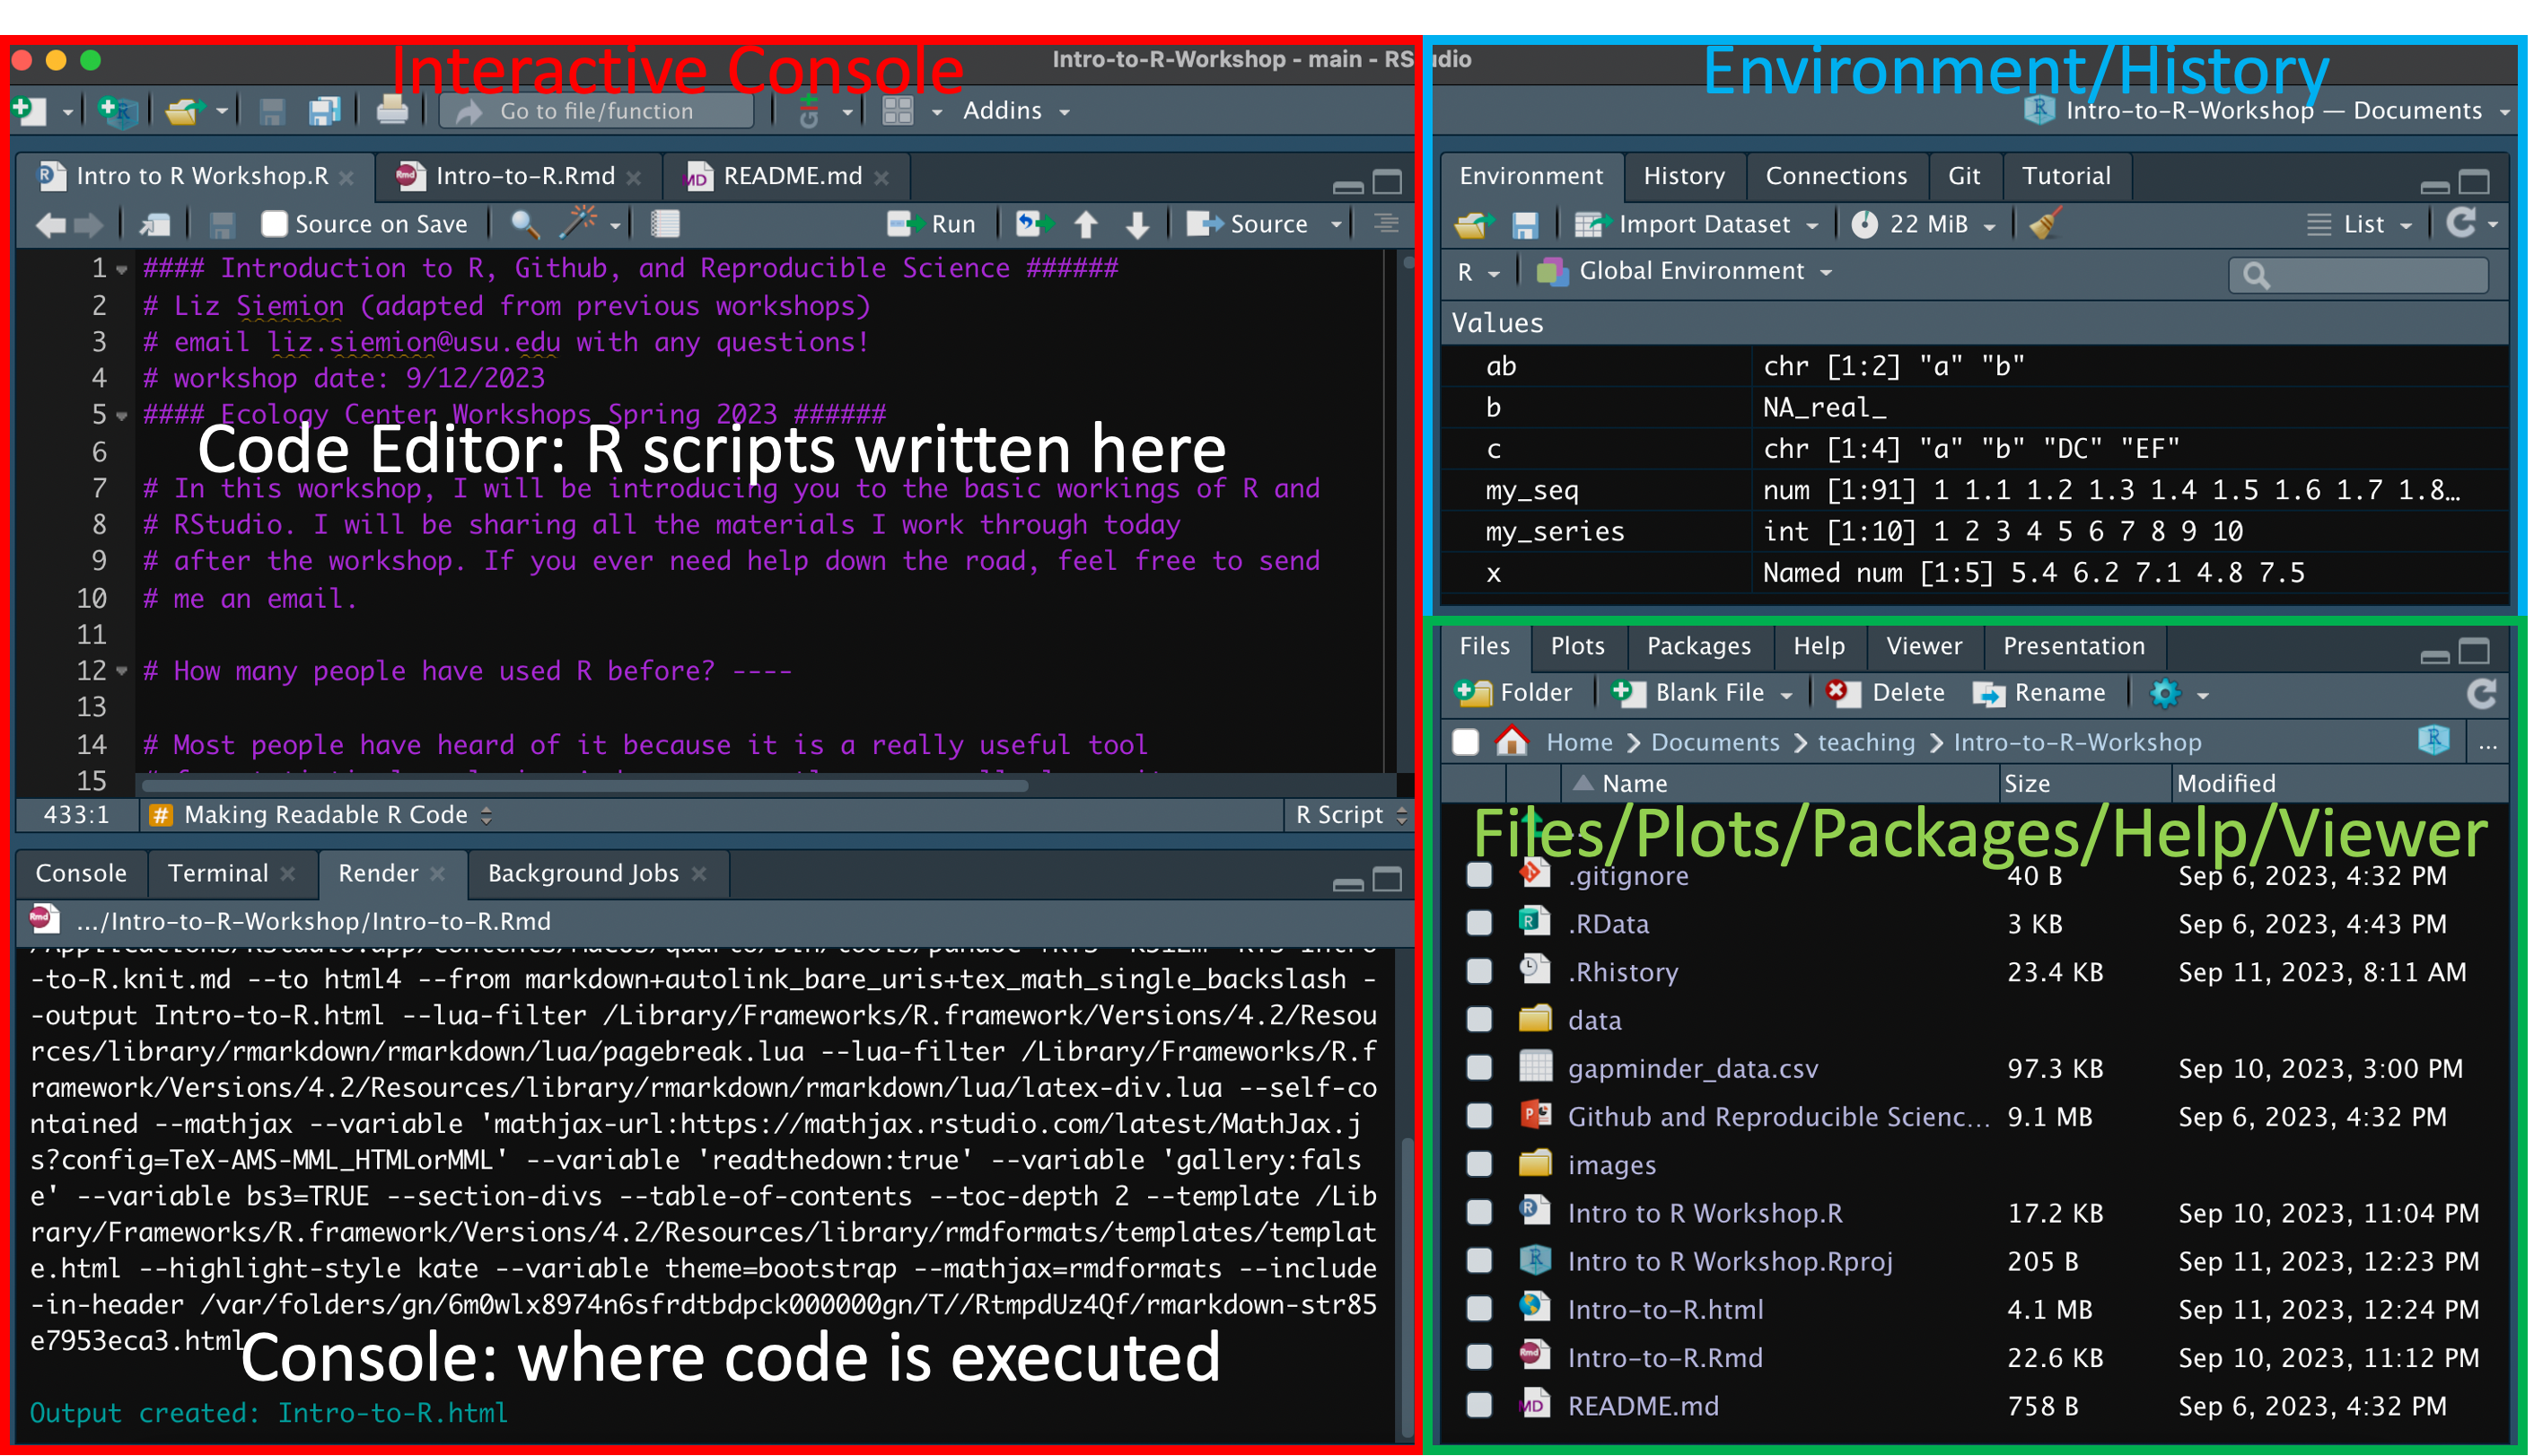
\includegraphics[keepaspectratio]{./docs/files/RStudio.png}}

\begin{enumerate}
\def\labelenumi{\arabic{enumi})}
\tightlist
\item
  \textbf{The Interactive R Console (entire left)}
\end{enumerate}

\begin{itemize}
\tightlist
\item
  The top-left panel in RStudio is the code editor, where you write and save your code. When you run a line of code from the code editor (i.e.~script), the output appears in the Console (bottom-left panel). While you can type and run code directly in the Console, it won't be saved when you close R unless you explicitly save your R history. That's why it's best to write your code in the code editor---so you have a permanent, editable copy---and send lines to the Console to execute as needed.
\end{itemize}

\begin{enumerate}
\def\labelenumi{\arabic{enumi})}
\setcounter{enumi}{1}
\tightlist
\item
  \textbf{Environment/History (tabbed in upper right)}
\end{enumerate}

\begin{itemize}
\tightlist
\item
  Environment: collection of objects (i.e.~variables, data frames, functions, etc.) that we define during our R session
\item
  History: a record of every line of code executed during the session
\end{itemize}

\begin{enumerate}
\def\labelenumi{\arabic{enumi})}
\setcounter{enumi}{2}
\tightlist
\item
  \textbf{Files/Plots/Packages/Help/Viewer (tabbed in lower right)}
\end{enumerate}

\begin{itemize}
\tightlist
\item
  \textbf{Files} shows all the files in your working directory. A \textbf{working directory} is essentially the default folder that R is reading data from/putting output into. We will go through setting the working directory below. You can also create, delete, and rename files and folders from this tab.
\item
  \textbf{Plots} displays figures that you generate
\item
  \textbf{Packages} displays any packages you have downloaded and installed in R. If there is a check mark next to a package, it means you've loaded it into your current R session
\item
  \textbf{Help} will show you a description of functions. To get a function description, simply run \texttt{?} followed by the function name. For example, \texttt{?setwd()} will show me the documentation for the \texttt{setwd()} function.
\item
  \textbf{Viewer} displays interactive or web-based content
\item
  \textbf{Presentation} displays slide-style documents created using R Markdown
\end{itemize}

\section{RStudio Projects}\label{rstudio-projects}

Now that we understand the basics of RStudio, let's create an RStudio Project that will live in the directory folder of the project. RStudio Projects are a self-contained, portable work space where you can have your data, code, and output all in one place. RStudio Projects are also great to use for reproducibility because they are self-contained and easy to share with collaborators. This means you can compress the entire RStudio Project into a ZIP file and share it with a collaborator, who should then be able to run your code and reproduce the same results. Let's go through how to set up an RStudio Project.

\textbf{Steps for Making an RProject}

\pandocbounded{\includegraphics[keepaspectratio]{./docs/files/RProject.png}}

\begin{enumerate}
\def\labelenumi{\arabic{enumi})}
\tightlist
\item
  Open the \texttt{File} menu from the upper left.
\item
  Select \texttt{Existing\ Directory} since we have already set up our project's directory
\item
  Navigate to the directory folder
\item
  Select \texttt{Create\ Project}
\end{enumerate}

Each time you open this RStudio project, the working directory is automatically set to the \texttt{IntroR} folder, where the project is saved. This means you don't need to manually set the working directory, as RStudio Projects handle it for you, helping keep your files and code organized and consistent.

For example, if my RStudio Project is located in C:/Teaching/IntroR/, my working directory is also located C:/Teaching/IntroR/.

\begin{center}\rule{0.5\linewidth}{0.5pt}\end{center}

\textbf{\texttt{EXERCISE\ 2:\ CREATE\ AN\ RSTUDIO\ PROJECT}}

\begin{enumerate}
\def\labelenumi{\arabic{enumi}.}
\tightlist
\item
  Create an RStudio PRoject in your \texttt{IntroR} folder.
\item
  Set a new editor theme. To change the editor theme, go to \textbf{Tools \textgreater{} Global Options}, click on the \textbf{Appearance tab}, and choose a new \textbf{editor theme} from the list. Each theme will be previewed in the right window.
\end{enumerate}

\begin{center}\rule{0.5\linewidth}{0.5pt}\end{center}

\chapter{File paths}\label{file}

To manually set the working directory or load a file from a specific location, it's important to understand how file paths work.

\section{What is a file path?}\label{what-is-a-file-path}

Your computer organizes files using a system of nested folders (i.e.~directory structure), where each folder can contain other folders or files.

Image from R for Epidemiology (\url{https://www.r4epi.com})

File paths are addresses to different locations (e.g.~files, documents) within this nested framework. They represents the order of nested folders that the computer must go through to find that particular item. Each folder is separated by a slash. We can use \texttt{Absolute} or \texttt{Relative} file paths in R to locate files. Knowing the file path is important when you need to set your working directory. See \href{https://www.r4epi.com/file-paths}{this website} for a detailed explanation.

\section{Different separators between operating systems}\label{different-separators-between-operating-systems}

Different operating systems use different separators between folders of a file path.

\begin{itemize}
\tightlist
\item
  On windows, it is \texttt{\textbackslash{}} or \texttt{//}
\item
  On Mac/Linux, it is \texttt{/}
\end{itemize}

R uses the / as the folder separator, even on Windows. So if you copy a file path from File Explorer (which uses ), be sure to either replace all backslashes () with forward slashes (/), or use double backslashes (\textbackslash) so R can read the path correctly.

\section{Absolute and Relative file paths}\label{absolute-and-relative-file-paths}

We can use \texttt{Absolute} or \texttt{Relative} file paths to give R directions to where we want to go.

\textbf{Absolute Paths:} describe where a file is located relative to the root directory of the computer. This can be done on windows through right clicking the file path in windows explorer and selecting copy as text, or right clicking a file, holding the option key and selecting copy as path name on a macbook.

\begin{itemize}
\tightlist
\item
  Windows example:
  \texttt{C:/Users/Documents/Teaching/IntroR/data/Intro-to-R-Workshop.csv}
\item
  Macbook example:
  \texttt{/Users/lizsiemion/Documents/Teaching/IntroR/Intro-to-R-Workshop.csv}
\end{itemize}

\textbf{Relative Paths:} describe file location with respect to the current working directory. This just means that the file path starts with the location of the home directory.

\begin{itemize}
\tightlist
\item
  Windows example:
  \texttt{IntroR/data/Intro-to-R-Workshop.csv}
\item
  Macbook example:
  \texttt{IntroR/data/Intro-to-R-Workshop.csv}
\end{itemize}

\includegraphics[width=0.9\linewidth,height=\textheight,keepaspectratio]{./docs/files/RProjectFilePath.png})

It can be a bit cumbersome to work with absolute file paths. Since R Projects automatically sets the working directory as the project folder, we can use relative paths without any sort of additional set-up.

Using relative paths also makes our code more readable, and easier to share and maintain. If we want to set our working directory manually, we can either use absolute or relative file paths. I recommend not changing the working directory within your script, as this can limit reproducibility.

\begin{Shaded}
\begin{Highlighting}[]
\CommentTok{\# check working directory}
\FunctionTok{getwd}\NormalTok{() }
\CommentTok{\# Assign working directory to new location using absolute path}
\FunctionTok{setwd}\NormalTok{(}\StringTok{"/Users/lizsiemion/Documents/teaching/Intro{-}to{-}R{-}Workshop"}\NormalTok{)}
\CommentTok{\# Again, I do not recommend changing the working directory from an R project.}
\end{Highlighting}
\end{Shaded}

Artwork by Allison Horst

\section{Navigating outside the working directory}\label{navigating-outside-the-working-directory}

Let's say we want to load a csv file into R that is outside of our working directory subfolders. How might we do that with absolute or relative paths from our current working directory?

The absolute path is the full file path from our computer's root directory. If we want to use the relative path, we need tell R to go up a given number of parent folder levels from a working directory, and then to the given location within that parent folder. This can be accomplished using \texttt{../} syntax.

\texttt{./\ tells\ R\ to\ go\ to\ the\ folder\ of\ the\ working\ directory}

\texttt{../\ tells\ R\ to\ go\ to\ the\ parent\ folder\ of\ the\ working\ directory}

\texttt{../../\ tells\ R\ to\ go\ to\ the\ parent\ folder\ of\ the\ parent\ folder\ of\ the\ working\ directory}

Let's look at an example. Say our folder structure resembles the structure below and our RProject is located in the Intro-to-R-Workshop folder.

\includegraphics[width=0.5\linewidth,height=\textheight,keepaspectratio]{./docs/files/folder_hierarchy.png}

\begin{itemize}
\item
  \textbf{Step 1:} How many parent levels do we need to move up?

  \begin{itemize}
  \tightlist
  \item
    Looks like we need to move up 1 level to the teaching folder \texttt{../}, and another level up to the Documents folder \texttt{../}.
  \end{itemize}
\item
  \textbf{Step 2:} Now that we are in the Documents folder, what is the relative path to to the \texttt{example\_file.txt}?

  \begin{itemize}
  \item
    We need to go into the Coursework folder, and then the EcologyCenter folder, where
    \texttt{example\_file.txt} is ultimately located.

    \texttt{Coursework/EC-tidyverse-workshop-main/example\_file.txt}
  \end{itemize}
\item
  By combining steps 1 and 2, we've create the relative file path and can load the \texttt{example\_file.txt} into our environment with \texttt{read.csv()}.

  \texttt{read.csv("../../Coursework/ecologycenter/example\_file.txt")}
\end{itemize}

\begin{center}\rule{0.5\linewidth}{0.5pt}\end{center}

\section{Using the Tab Shortcut in RStudio}\label{using-the-tab-shortcut-in-rstudio}

The Tab shortcut in RStudio is a powerful shortcut that helps you write code faster and with fewer errors. It's especially helpful for auto-completing file paths, function names, object names, and more. When you're loading a file (e.g., using read.csv()), you can use the Tab key to help you find and insert the correct relative file path.

For example: \texttt{read.csv("data/}

Then press the Tab key. A drop down list will appear showing the contents of the data/ folder (if it exists). You can then use the arrow keys to select a file and select Enter to insert it into the code. The Tab key shortcut helps avoid typos and ensures you're referencing the correct file.

\pandocbounded{\includegraphics[keepaspectratio]{./docs/files/TabShortcut.png}}

\begin{center}\rule{0.5\linewidth}{0.5pt}\end{center}

\textbf{\texttt{EXERCISE\ 1:\ FILE\ PATHS}}

\begin{enumerate}
\def\labelenumi{\arabic{enumi}.}
\tightlist
\item
  Enter \texttt{getwd()} into the console to return the absolute file path
\item
  Use a relative file path to load the bighorn capture table using read.csv(``TYPE\_RELATIVE\_FILE\_PATH'').
  The read.csv() function tells R to load the CSV file into your Environment. Make sure the file path is placed inside quotes and within the parentheses. Tip: Try using the Tab key after typing the opening quote to help you navigate and generate the correct relative file path.
\end{enumerate}

\begin{center}\rule{0.5\linewidth}{0.5pt}\end{center}

\chapter{Tidy Data}\label{tidy-data}

\section{Tidy Data}\label{tidy-data-1}

Illustrations from the Openscapes blog Tidy Data for reproducibility, efficiency, and collaboration by Julia Lowndes and Allison Horst

\section{Document your code}\label{document-your-code}

It's good practice to include comments and documentation explaining what your code is doing and why. This makes it easier to understand your code, which can be useful if your code is complex or you haven't worked with it in awhile. Good documentation helps with debugging, collaboration, and keeping your workflow organized and reproducible. RMarkdown and README files are useful methods for documenting your progress.

\section{Rows for Observations, Columns for Variables}\label{rows-for-observations-columns-for-variables}

When organizing your data, it is best to keep it in long format, where each row represents a new observation and each column represents a new variable.

\section{Problemmatic Practices}\label{problemmatic-practices}

\begin{itemize}
\tightlist
\item
  Avoid putting units in cells
\item
  Do not use white spaces in column names
\item
  Recognize the difference between zero and a missing value
\item
  Ensure that you consistently format your values in your spreadsheets
\end{itemize}

\chapter{Using R}\label{using-r}

\section{Installing Packages}\label{packages}

Sometimes you will want to use tools that are not built into the baseR code. You can download these tools from R repositories as \texttt{packages}. A package is a collection of functions, data, and documentation designed to accomplish a particular task. An R package can help with tasks such as data visualization, statistical modeling, or data cleaning. You can install an R package through the RStudio interface, or through entering code into the console.

\begin{Shaded}
\begin{Highlighting}[]
\FunctionTok{install.packages}\NormalTok{(}\StringTok{"amt"}\NormalTok{) }\CommentTok{\# install a new package}
\FunctionTok{library}\NormalTok{(amt) }\CommentTok{\# call a package you previously downloaded}
\end{Highlighting}
\end{Shaded}

\begin{center}\rule{0.5\linewidth}{0.5pt}\end{center}

\textbf{\texttt{EXERCISE}}

Load Tidyverse package using RStudio

\begin{enumerate}
\def\labelenumi{\arabic{enumi}.}
\tightlist
\item
  Select \texttt{Packages}
\item
  Select \texttt{Install}
\item
  Type \texttt{tidyverse}
\item
  Select \texttt{Install}
\item
  Bonus: Install tidyverse in the code editor using the example code above.
\end{enumerate}

\textbf{We will go over what tidyverse is later on in this course}

\begin{center}\rule{0.5\linewidth}{0.5pt}\end{center}

If two different packages contain functions with the same name, R will mask one with the other based on the order they are loaded. To avoid confusion, you can explicitly tell R which package to use with the \texttt{package::function()} format. For example, the \texttt{filter()} function exists in both \texttt{stats} and \texttt{dplyr} packages. If you specifically want the version from \texttt{dplyr}, you can write \texttt{dplyr::filter()} in your code. We will talk more about this later on.

\section{Using Comments}\label{using-comments}

Use the \texttt{\#} to tell R you are making a comment. Comments are used to explain code and allow someone unfamiliar with your code to follow more easily. Commenting can also be used to prevent R from running specific lines of code since R ignores anything that follows the \texttt{\#} mark.

\begin{Shaded}
\begin{Highlighting}[]
\CommentTok{\# 567*5 tells R that 567*5 is a comment, and so R knows not to execute this line of code.}
\end{Highlighting}
\end{Shaded}

Sometimes you want to comment out large sections of code, and this can be done using \texttt{control\ +\ shift\ +\ c} on windows or \texttt{command\ +\ shift\ +\ c} on a Macbook.

\begin{center}\rule{0.5\linewidth}{0.5pt}\end{center}

\textbf{\texttt{EXERCISE}}

\begin{enumerate}
\def\labelenumi{\arabic{enumi}.}
\tightlist
\item
  Create a new script (\textbf{File \textgreater{} New File \textgreater{} R Script})
\item
  In the first line, type \texttt{\#\ Intro\ R}
\item
  On line 2, type \texttt{1\ +\ 1}
\item
  Select \texttt{Run} in the upper right corner of the console. You can also use the shortcut \texttt{control\ +\ enter} on Windows and \texttt{command\ +\ enter} on a Macbook. If the keyboard shortcuts aren't working, navigate to \textbf{Tools \textgreater{} Modify Keyboard Shortcuts }, type \textbf{Run Current Line or Section} into the search bar, double-click the shortcut, remove the current key combination, and enter your preferred shortcut.
\end{enumerate}

\begin{center}\rule{0.5\linewidth}{0.5pt}\end{center}

\section{Functions}\label{functions}

A function is a defined script that is used to accomplish a particular task. Functions use an input to give a desired output. R provides built-in functions, such as \texttt{mean()}, \texttt{sum()}, and \texttt{plot()}, which perform commonly used operations. Every function has arguments that determine what kind of inputs are needed to make the function run.

\begin{itemize}
\tightlist
\item
  Arguments: information that goes inside the parenthesis to tell the function what to do. For example, when we used the \texttt{seq} function, the arguments are \texttt{from}, \texttt{to}, and \texttt{by}. Many arguments have a default value, which is a value that is automatically used for an argument if you don't provide your own. For example, in \texttt{seq()}, the default value for the \texttt{from} argument is 1.
\item
  Pass: We pass a value to a function argument. We can pass the value 1 to the argument \texttt{from}, and the value 10 to the argument \texttt{to} and the value 0.1 to the argument \texttt{by}.
\item
  Return: This is the terminology to say that the function gives us an output. So with the \texttt{seq(from\ =\ 1,\ to\ =\ 10,\ by\ =\ 0.1)}, the function returns a sequence of numbers
\end{itemize}

\begin{Shaded}
\begin{Highlighting}[]
\NormalTok{function\_name }\OtherTok{\textless{}{-}} \ControlFlowTok{function}\NormalTok{(arg1, arg2) \{ }\CommentTok{\# arg1 and arg2 are inputs}
  \CommentTok{\# Code that processes the inputs}
\NormalTok{  result }\OtherTok{\textless{}{-}}\NormalTok{ arg1 }\SpecialCharTok{+}\NormalTok{ arg2}
  \FunctionTok{return}\NormalTok{(result)  }\CommentTok{\# return() provides the output of the function}
\NormalTok{\}}
\end{Highlighting}
\end{Shaded}

The order of arguments in a function call matters, especially when you don't name them. To avoid confusion, it's often helpful to explicitly name the arguments. You can use the help function \texttt{?} to check the correct usage of a function. For example, to learn more about the \texttt{rep()} function, you can execute the command \texttt{?rep} in your Console.

Additionally, you can define your own functions to solve specific problems and use them repeatedly in your code without having to repeat the code multiple times. For example, if you need to convert elevation from meters to feet in several places in your script, you can write a function to do it once and then use that function whenever you need it. Functions are an essential part of R programming, as they allow for cleaner, more efficient, and modular code. Although we won't be covering custom functions in this course, it's important to note that creating your own functions is a common and useful practice in programming.

\begin{Shaded}
\begin{Highlighting}[]
\CommentTok{\# Write a function to convert a column of elevation in meters to feet}
\NormalTok{convert\_elevation\_to\_feet }\OtherTok{\textless{}{-}} \ControlFlowTok{function}\NormalTok{(elev\_m) \{ }\CommentTok{\# vector of elevation in meters is input (argument)}
\NormalTok{  elev\_ft }\OtherTok{\textless{}{-}}\NormalTok{ elev\_m }\SpecialCharTok{*} \FloatTok{3.28084} \CommentTok{\# code to process elevation in meters to feet}
  \FunctionTok{return}\NormalTok{(elev\_ft) }\CommentTok{\# return output of function}
\NormalTok{\}}
\end{Highlighting}
\end{Shaded}

\begin{center}\rule{0.5\linewidth}{0.5pt}\end{center}

\textbf{\texttt{EXERCISE}}

\begin{enumerate}
\def\labelenumi{\arabic{enumi}.}
\tightlist
\item
  Use the \texttt{?} function to look up the seq() function.
\item
  Why does \texttt{seq(from\ =\ 1,\ by\ =\ 3)} return a sequence successfully, while \texttt{seq(from\ =\ 40,\ by\ =\ 3)} results in an error? What is causing the difference in behavior? Hint: look up \texttt{seq} using the help function. Are there any default values? How might that affect the behavior of the function?
\end{enumerate}

\begin{center}\rule{0.5\linewidth}{0.5pt}\end{center}

\section{Use R as a calculator}\label{use-r-as-a-calculator}

Remember, order of operations matters. The order is the same as you learned back in school.

From highest to lowest precedence:

\begin{longtable}[]{@{}lll@{}}
\toprule\noalign{}
Operator & Symbol(s) & Description \\
\midrule\noalign{}
\endhead
\bottomrule\noalign{}
\endlastfoot
Parentheses & \texttt{(} \texttt{)} & Controls the order of operations \\
Exponents & \texttt{\^{}}, \texttt{**} & Raises a number to a power \\
Divide & \texttt{/} & Division \\
Multiply & \texttt{*} & Multiplication \\
Add & \texttt{+} & Addition \\
Subtract & \texttt{-} & Subtraction \\
\end{longtable}

\begin{Shaded}
\begin{Highlighting}[]
\DecValTok{1} \SpecialCharTok{+} \DecValTok{100} \CommentTok{\# performs addition}
\end{Highlighting}
\end{Shaded}

\begin{verbatim}
## [1] 101
\end{verbatim}

\begin{Shaded}
\begin{Highlighting}[]
\DecValTok{3} \SpecialCharTok{+} \DecValTok{5} \SpecialCharTok{*} \DecValTok{2} \CommentTok{\# performs multiplication before addition}
\end{Highlighting}
\end{Shaded}

\begin{verbatim}
## [1] 13
\end{verbatim}

\begin{Shaded}
\begin{Highlighting}[]
\NormalTok{(}\DecValTok{3} \SpecialCharTok{+} \DecValTok{5}\NormalTok{) }\SpecialCharTok{*} \DecValTok{2} \CommentTok{\# performs addition in () before multiplication }
\end{Highlighting}
\end{Shaded}

\begin{verbatim}
## [1] 16
\end{verbatim}

\begin{Shaded}
\begin{Highlighting}[]
\DecValTok{2}\SpecialCharTok{/}\DecValTok{10000} \CommentTok{\# division}
\end{Highlighting}
\end{Shaded}

\begin{verbatim}
## [1] 2e-04
\end{verbatim}

\begin{Shaded}
\begin{Highlighting}[]
\DecValTok{2} \SpecialCharTok{\^{}} \DecValTok{3} \CommentTok{\# exponentiation: 2 raised to the power of 3}
\end{Highlighting}
\end{Shaded}

\begin{verbatim}
## [1] 8
\end{verbatim}

\section{Use R to compare things}\label{use-r-to-compare-things}

To compare things in R, we use logical operators. Below is a brief list.

\begin{longtable}[]{@{}ll@{}}
\toprule\noalign{}
Operator & Meaning \\
\midrule\noalign{}
\endhead
\bottomrule\noalign{}
\endlastfoot
\texttt{==} & is equal to \\
\texttt{\textgreater{}} & greater than \\
\texttt{\textless{}} & less than \\
\texttt{\textgreater{}=} & greater than or equal to \\
\texttt{\textless{}=} & less than or equal to \\
\texttt{!} & not \\
\texttt{\textbar{}} & or \\
\texttt{\%in\%} & is contained in \\
\end{longtable}

Let's go through a few examples of using logical operators. Notice how R evaluates each of these lines of code as TRUE or FALSE. We are essentially asking R if the above comparison is TRUE or FALSE. We will go over \texttt{\%in\%} later in this class.

\begin{Shaded}
\begin{Highlighting}[]
\DecValTok{1} \SpecialCharTok{==} \DecValTok{9}  \CommentTok{\# equality (note two equals signs, read as "is equal to")}
\end{Highlighting}
\end{Shaded}

\begin{verbatim}
## [1] FALSE
\end{verbatim}

\begin{Shaded}
\begin{Highlighting}[]
\DecValTok{1} \SpecialCharTok{!=} \DecValTok{1}  \CommentTok{\# inequality (read as "is not equal to")}
\end{Highlighting}
\end{Shaded}

\begin{verbatim}
## [1] FALSE
\end{verbatim}

\begin{Shaded}
\begin{Highlighting}[]
\DecValTok{1} \SpecialCharTok{\textless{}} \DecValTok{2}  \CommentTok{\# less than}
\end{Highlighting}
\end{Shaded}

\begin{verbatim}
## [1] TRUE
\end{verbatim}

\begin{Shaded}
\begin{Highlighting}[]
\DecValTok{1} \SpecialCharTok{\textless{}=} \DecValTok{1}  \CommentTok{\# less than or equal to}
\end{Highlighting}
\end{Shaded}

\begin{verbatim}
## [1] TRUE
\end{verbatim}

\begin{center}\rule{0.5\linewidth}{0.5pt}\end{center}

\textbf{\texttt{EXERCISE}}

\begin{enumerate}
\def\labelenumi{\arabic{enumi}.}
\tightlist
\item
  In your code editor, enter the following lines of code. Then run them to view each line of code's output in your console.

  \begin{enumerate}
  \def\labelenumii{\alph{enumii}.}
  \tightlist
  \item
    67 * 9
  \item
    7 + 9 + 10
  \item
    4399 - 871 * (9 + 1)
  \end{enumerate}
\item
  Evaluate whether the following logical conditions are TRUE or FALSE

  \begin{enumerate}
  \def\labelenumii{\alph{enumii}.}
  \tightlist
  \item
    \texttt{(380*3)\ ==\ (190*6)}
  \item
    \texttt{567\ \textgreater{}\ 890}
  \item
    \texttt{30\ \textgreater{}=\ (27\ +\ 1\ +\ 2)}
  \end{enumerate}
\item
  Bonus: What is wrong with the following code?

  \begin{enumerate}
  \def\labelenumii{\alph{enumii}.}
  \tightlist
  \item
    Type \texttt{87(9\ +\ 1)} into your console
  \item
    Execute that specific line of code by placing the cursor on that line and selecting \texttt{Run}.
  \item
    What error do you see? What do you think is happening? How might you fix this?
  \end{enumerate}
\end{enumerate}

\begin{center}\rule{0.5\linewidth}{0.5pt}\end{center}

\section{Use R to assign objects}\label{r-objects}

Objects are a bit of an abstract concept. All you really need to know for now is that objects are things that we make in R that can take on a variety of structures with different data types, and when we assign them a name, they get saved in our global environment. \textbf{Objects are data structures with associated data attributes.}

Object assignment lets us assign a name to a value, making it easier to use later. This helps avoid repeating code. We assign a value to a variable using the assignment arrow \texttt{\textless{}-} or the \texttt{=} so that R recognizes the name as a reference to the object. So when we run, \texttt{x\ \textless{}-\ 6}, it reads make x contain 6 It's recommended to use the \texttt{\textless{}-} since the \texttt{=} can get mixed up with assigning values to function arguments. Once we assign an object to a variable, it is stored in our global environment (upper right hand panel of RStudio).

\begin{Shaded}
\begin{Highlighting}[]
\NormalTok{x }\OtherTok{\textless{}{-}} \DecValTok{1}\SpecialCharTok{/}\DecValTok{40} \CommentTok{\# here we are telling R to assign 1/40 to the variable x so that it recognizes x as an object in our global environment}
\NormalTok{x }\OtherTok{\textless{}{-}}  \DecValTok{24} \CommentTok{\# variables can easily be re{-}assigned/over{-}written}
\NormalTok{y }\OtherTok{\textless{}{-}}\NormalTok{ x }\SpecialCharTok{*} \DecValTok{2} \CommentTok{\# We can use existing objeects in expressions to create new objects}

\FunctionTok{rm}\NormalTok{(y) }\CommentTok{\# you can also remove objects from the environment using the rm() function}
\end{Highlighting}
\end{Shaded}

\subsection{Variable names}\label{variable-names}

Variable names can contain letters, numbers, underscores and periods.
\textbf{They CANNOT start with a number OR contain any spaces.} Recall that R is case sensitive.

A few different conventions for longer variable names:

\begin{itemize}
\tightlist
\item
  periods.between.words
\item
  underscores\_between\_words
\item
  camelCaseToSeparateWords
\end{itemize}

Your choice of convention is up to you, \emph{JUST BE CONSISTENT}.

\begin{center}\rule{0.5\linewidth}{0.5pt}\end{center}

\textbf{\texttt{EXERCISE}}

\begin{enumerate}
\def\labelenumi{\arabic{enumi}.}
\tightlist
\item
  Assign \texttt{1+56} to a variable called \texttt{x1\_a}
\item
  Assign \texttt{sqrt(24)} to a variable called \texttt{x1\_b}. Use \texttt{?sqrt} to learn more about the \texttt{sqrt()} function. What is the name of the argument of the \texttt{sqrt()} function?
\item
  Bonus: Chained assignments. What happens when you execute \texttt{x3.c\ \textless{}-\ y3.c\ \textless{}-\ 9/10} into your console? Are \texttt{x3.c} and \texttt{y3.c} different or equal values?
\end{enumerate}

\begin{center}\rule{0.5\linewidth}{0.5pt}\end{center}

\section{Data Types (Modes)}\label{data-types}

There are 6 main classes of common data modes (i.e.~data types): \texttt{numeric}, \texttt{character}, \texttt{logical}, \texttt{integer}, \texttt{complex}, and \texttt{factor}. Data modes refers to the basic type of data stored in an object. For example, numeric mode stores numbers (integers or decimals), and character mode stores text. We typically only use \texttt{factor}, \texttt{numeric}, \texttt{character}, and \texttt{logical} data modes.

\begin{longtable}[]{@{}
  >{\raggedright\arraybackslash}p{(\linewidth - 4\tabcolsep) * \real{0.1529}}
  >{\raggedright\arraybackslash}p{(\linewidth - 4\tabcolsep) * \real{0.5176}}
  >{\raggedright\arraybackslash}p{(\linewidth - 4\tabcolsep) * \real{0.3294}}@{}}
\toprule\noalign{}
\begin{minipage}[b]{\linewidth}\raggedright
Mode
\end{minipage} & \begin{minipage}[b]{\linewidth}\raggedright
Description
\end{minipage} & \begin{minipage}[b]{\linewidth}\raggedright
Example
\end{minipage} \\
\midrule\noalign{}
\endhead
\bottomrule\noalign{}
\endlastfoot
factor & Categorical data (special class of integer with labels stored as characters) & Levels: ``Sheep'', ``Lion'', ``Deer'' (internally stored as: 1, 2, 3) \\
numeric & Numbers (includes integers and decimals) & 3.14, 42 \\
character & Text strings & ``Lion180'' \\
logical & TRUE or FALSE values & TRUE, FALSE \\
\end{longtable}

To ask R what \texttt{class} a data mode or object is, we use the \texttt{class()} function.

\begin{Shaded}
\begin{Highlighting}[]
\FunctionTok{class}\NormalTok{(}\FloatTok{1.11}\NormalTok{) }\CommentTok{\# numeric: any real number}
\FunctionTok{class}\NormalTok{(}\DecValTok{1}\DataTypeTok{L}\NormalTok{) }\CommentTok{\# integer: any integer. The L suffix forces the number to be an integer}
\FunctionTok{class}\NormalTok{(}\ConstantTok{TRUE}\NormalTok{) }\CommentTok{\# logical: binary TRUE or FALSE }
\CommentTok{\# You can have data that look essentially the same, but have different classes. }
\FunctionTok{class}\NormalTok{(}\StringTok{\textquotesingle{}1\textquotesingle{}}\NormalTok{) }\CommentTok{\# character: words; "" denote words}
\FunctionTok{class}\NormalTok{(}\DecValTok{1}\NormalTok{) }\CommentTok{\# numeric; any real number}
\FunctionTok{class}\NormalTok{(}\FunctionTok{factor}\NormalTok{(}\StringTok{"1a"}\NormalTok{)) }\CommentTok{\# factor: denotes categorical variables, they can be words or numbers}
\end{Highlighting}
\end{Shaded}

You can coerce to a desired data type, as long as they follow the rules
using the functions \texttt{as.\textless{}desired\ data\ type\textgreater{}}

\textbf{Coercion Hierarchy (from general to specific): Character → Numeric → Logical}

\begin{enumerate}
\def\labelenumi{\arabic{enumi}.}
\tightlist
\item
  character most general: anything can be turned into a character by adding ``quotes''

  \begin{itemize}
  \tightlist
  \item
    e.g.~as.character(TRUE) → ``TRUE''
  \end{itemize}
\item
  numeric: can read integer and logical types as numbers. Cannot reliably coerce character strings unless they represent valid numbers

  \begin{itemize}
  \tightlist
  \item
    e.g.~``3.14'' → 3.14, TRUE → 1; FALSE → 0; ``S438'' → NA
  \end{itemize}
\item
  logical: most specific, cannot turn turn character or numeric into a logical type without correctly specifying the value. Coercing a character or invalid numeric value to logical produces an NA

  \begin{itemize}
  \tightlist
  \item
    e.g.~as.logical(``sheep'' → NA); as.logical(3.14 → TRUE)
  \end{itemize}
\item
  Factor: (special case) internally stored as integers with labels. To get the original numeric value, you must coerce factor to character first, then to numeric. Direct coercion from factor to numeric returns internal integer codes (not labels)
\end{enumerate}

\begin{Shaded}
\begin{Highlighting}[]
\CommentTok{\# create numeric object}
\NormalTok{a }\OtherTok{\textless{}{-}} \FloatTok{45.6}
\FunctionTok{class}\NormalTok{(a)}
\end{Highlighting}
\end{Shaded}

\begin{verbatim}
## [1] "numeric"
\end{verbatim}

\begin{Shaded}
\begin{Highlighting}[]
\CommentTok{\# Convert from numeric to character}
\NormalTok{a\_character }\OtherTok{\textless{}{-}} \FunctionTok{as.character}\NormalTok{(a)}
\FunctionTok{class}\NormalTok{(a\_character)}
\end{Highlighting}
\end{Shaded}

\begin{verbatim}
## [1] "character"
\end{verbatim}

\begin{Shaded}
\begin{Highlighting}[]
\CommentTok{\# Create factored object}
\NormalTok{lion }\OtherTok{\textless{}{-}} \FunctionTok{factor}\NormalTok{(}\FunctionTok{c}\NormalTok{(}\StringTok{"194"}\NormalTok{, }\StringTok{"180"}\NormalTok{), }\AttributeTok{levels =} \FunctionTok{c}\NormalTok{(}\StringTok{"194"}\NormalTok{, }\StringTok{"180"}\NormalTok{)) }\CommentTok{\# The levels must match the exact format of the values}
\NormalTok{lion }\CommentTok{\# print value into console}
\end{Highlighting}
\end{Shaded}

\begin{verbatim}
## [1] 194 180
## Levels: 194 180
\end{verbatim}

\begin{Shaded}
\begin{Highlighting}[]
\FunctionTok{as.character}\NormalTok{(lion) }\CommentTok{\# coerced to character}
\end{Highlighting}
\end{Shaded}

\begin{verbatim}
## [1] "194" "180"
\end{verbatim}

\begin{Shaded}
\begin{Highlighting}[]
\FunctionTok{as.numeric}\NormalTok{(lion) }\CommentTok{\# coerced to numeric}
\end{Highlighting}
\end{Shaded}

\begin{verbatim}
## [1] 1 2
\end{verbatim}

You can also coerce from factor to character to numeric in one call

\begin{Shaded}
\begin{Highlighting}[]
\FunctionTok{as.numeric}\NormalTok{(}\FunctionTok{as.character}\NormalTok{(lion))}
\end{Highlighting}
\end{Shaded}

\begin{verbatim}
## [1] 194 180
\end{verbatim}

A common mistake in R is using data of the wrong type. In the example below, an error occurs because R cannot convert a character value into a numeric one. It's important to ensure that the data you're working with is of the correct type.

\begin{Shaded}
\begin{Highlighting}[]
\CommentTok{\# convert from character to numeric}
\NormalTok{L262 }\OtherTok{\textless{}{-}} \StringTok{"Lion262"}
\NormalTok{L262\_numeric }\OtherTok{\textless{}{-}} \FunctionTok{as.numeric}\NormalTok{(L262)}
\end{Highlighting}
\end{Shaded}

\begin{verbatim}
## Warning: NAs introduced by coercion
\end{verbatim}

\begin{Shaded}
\begin{Highlighting}[]
\NormalTok{L262\_numeric}
\end{Highlighting}
\end{Shaded}

\begin{verbatim}
## [1] NA
\end{verbatim}

\begin{center}\rule{0.5\linewidth}{0.5pt}\end{center}

\textbf{\texttt{EXERCISE}}

\begin{enumerate}
\def\labelenumi{\arabic{enumi}.}
\tightlist
\item
  Assign \texttt{"S437"} to a variable called \texttt{sheep} (\texttt{sheep\ \textless{}-\ "S437"}). Make sure to include the \texttt{""}.
\item
  What type of data class is sheep? This can be figured out by doing \texttt{class(sheep)}
\item
  Create an object with a value of \texttt{45}. Coerce to a character class using \texttt{as.character()}.
\item
  Create the following objects: \texttt{S1\ \textless{}-\ as.numeric(as.character(1))} and \texttt{S2\ \textless{}-\ as.logical(as.numeric("1"))}.
\item
  Do the values change? Why or why not? Think about this answer in the context of the coercian hierarchy.
\item
  Bonus: What happens when you execute \texttt{sheep\ \textless{}-\ S437} without \texttt{""}? Explain the error.
\end{enumerate}

\begin{center}\rule{0.5\linewidth}{0.5pt}\end{center}

\section{Other Object Types}\label{other-object-types}

R includes many other object types that we won't cover in detail during this course. For instance, spatial object types are used to represent and work with geographic data. Spatial objects can take on different data types depending on if they are from the \texttt{sp} or \texttt{sf} package.

\section{Data Structure Classes}\label{data-classes}

Remember when we talked about objects as data with attributes? Well, R offers several ways to store data, depending on what kind of structure you need. The most common types are vectors, data frames, and lists. Each of these can store different types of information and are useful in different contexts when working with data. Think of them as different types of containers for data that are designed to hold and organize data in specific ways. We will be discussing \texttt{Scalar}, \texttt{Vector}, \texttt{Data\ Frames}, \texttt{Matrices}, and \texttt{Lists}. Below is a summary of each of these data structures, and we will also go through each of these individually.

\begin{longtable}[]{@{}
  >{\raggedright\arraybackslash}p{(\linewidth - 8\tabcolsep) * \real{0.0884}}
  >{\raggedright\arraybackslash}p{(\linewidth - 8\tabcolsep) * \real{0.3260}}
  >{\raggedright\arraybackslash}p{(\linewidth - 8\tabcolsep) * \real{0.1657}}
  >{\raggedright\arraybackslash}p{(\linewidth - 8\tabcolsep) * \real{0.0939}}
  >{\raggedright\arraybackslash}p{(\linewidth - 8\tabcolsep) * \real{0.3260}}@{}}
\toprule\noalign{}
\begin{minipage}[b]{\linewidth}\raggedright
Data Structure
\end{minipage} & \begin{minipage}[b]{\linewidth}\raggedright
Description
\end{minipage} & \begin{minipage}[b]{\linewidth}\raggedright
Can Contain Different Types?
\end{minipage} & \begin{minipage}[b]{\linewidth}\raggedright
Dimensions
\end{minipage} & \begin{minipage}[b]{\linewidth}\raggedright
Example
\end{minipage} \\
\midrule\noalign{}
\endhead
\bottomrule\noalign{}
\endlastfoot
Scalar & A single value (a vector of length 1) & No & 1 (length = 1) & \texttt{x\ \textless{}-\ 42} \\
Vector & A sequence of elements of the same type & No & 1 (length \textgreater{} 1) & \texttt{c(1,\ 2,\ 3)} \\
Data Frame & Table-like structure with columns of equal length & Yes (by column) & 2 (rows × cols) & \texttt{data.frame(a\ =\ 1:3,\ b\ =\ c("x",\ "y",\ "z"))} \\
Tibble & A modern, enhanced version of a data frame from the \textbf{tidyverse}, with stricter handling and improved printing & Yes (by column) & 2 (rows × cols) & \texttt{tibble(a\ =\ 1:3,\ b\ =\ c("x",\ "y",\ "z"))} \\
Matrix & 2D array with all elements of the same type & No & 2 (rows × cols) & \texttt{matrix(1:6,\ nrow\ =\ 2)} \\
List & A collection of elements that can be of different types & Yes & 1 (named or not) & \texttt{list(name\ =\ "A",\ age\ =\ 25,\ scores\ =\ c(1,2,3))} \\
\end{longtable}

\subsection{Scalar}\label{scalar}

A scalar object contains only one element (length is 1). An element is an individual value or item within a data structure

\begin{Shaded}
\begin{Highlighting}[]
\NormalTok{x }\OtherTok{\textless{}{-}} \DecValTok{3}
\end{Highlighting}
\end{Shaded}

\begin{center}\rule{0.5\linewidth}{0.5pt}\end{center}

\textbf{\texttt{EXERCISE}}

\begin{enumerate}
\def\labelenumi{\arabic{enumi}.}
\tightlist
\item
  Create a scalar object named my\_scalar and assign it the value 87
\end{enumerate}

\begin{center}\rule{0.5\linewidth}{0.5pt}\end{center}

\subsection{Vector}\label{vector}

A scalar object is a special case of a vector with a length of 1. A vector in R is essentially a collection of elements \textbf{of the same basic data type}. Each `thing' in the vector is called an element. You can combine values into one vector with different values using the concatenate function \texttt{c()}.

\begin{Shaded}
\begin{Highlighting}[]
\NormalTok{my.deer }\OtherTok{\textless{}{-}} \FunctionTok{c}\NormalTok{(}\StringTok{"GDL256"}\NormalTok{, }\StringTok{"RVD1011"}\NormalTok{, }\StringTok{"CDB567"}\NormalTok{)}
\end{Highlighting}
\end{Shaded}

You can also create an empty vector. If you don't specify a data type, R will default to logical, or, you can declare an empty vector of whatever type you like.

\begin{Shaded}
\begin{Highlighting}[]
\NormalTok{my\_vector }\OtherTok{\textless{}{-}} \FunctionTok{vector}\NormalTok{(}\AttributeTok{length =} \DecValTok{3}\NormalTok{, }\AttributeTok{mode =} \StringTok{"numeric"}\NormalTok{)}
\NormalTok{my\_vector  }\CommentTok{\# this is a logical vector}
\end{Highlighting}
\end{Shaded}

\begin{verbatim}
## [1] 0 0 0
\end{verbatim}

\begin{Shaded}
\begin{Highlighting}[]
\NormalTok{num\_vector }\OtherTok{\textless{}{-}} \FunctionTok{c}\NormalTok{(}\DecValTok{101}\NormalTok{, }\DecValTok{222}\NormalTok{, }\DecValTok{323}\NormalTok{, }\DecValTok{435}\NormalTok{, }\DecValTok{556}\NormalTok{) }\CommentTok{\# numeric vector}
\end{Highlighting}
\end{Shaded}

What happens when we add elements of different data types to a vector?

\begin{Shaded}
\begin{Highlighting}[]
\NormalTok{combine\_vector }\OtherTok{\textless{}{-}} \FunctionTok{c}\NormalTok{(}\DecValTok{211}\NormalTok{, }\StringTok{"CDB678"}\NormalTok{, }\ConstantTok{TRUE}\NormalTok{)}
\NormalTok{combine\_vector}
\end{Highlighting}
\end{Shaded}

\begin{verbatim}
## [1] "211"    "CDB678" "TRUE"
\end{verbatim}

\begin{Shaded}
\begin{Highlighting}[]
\FunctionTok{class}\NormalTok{(combine\_vector) }
\end{Highlighting}
\end{Shaded}

\begin{verbatim}
## [1] "character"
\end{verbatim}

R coerces all the elements in ``combine\_vector'' to character. It can't make \texttt{"CDB678"} into a number but it can turn \texttt{211} and \texttt{TRUE} into text strings (think about the coercion hierarchy)

You can also assign \texttt{NA} values to a vector of defined length as well. R is able to handle missing values, and these missing values are given \texttt{NA}. When you read in an csv file with empty cells, R will assign these values as NA. A \texttt{0} is not the same as \texttt{NA}, since R treats \texttt{0} as a numeric data class.

\begin{Shaded}
\begin{Highlighting}[]
\CommentTok{\# create a vector of 10 NA values}
\NormalTok{x }\OtherTok{\textless{}{-}} \FunctionTok{rep}\NormalTok{(}\ConstantTok{NA}\NormalTok{, }\DecValTok{10}\NormalTok{)}
\CommentTok{\# set the first element in x to be the number 0}
\NormalTok{x[}\DecValTok{1}\NormalTok{] }\OtherTok{\textless{}{-}} \DecValTok{0}
\CommentTok{\# test if zero is NA}
\FunctionTok{is.na}\NormalTok{(x)}
\end{Highlighting}
\end{Shaded}

\begin{verbatim}
##  [1] FALSE  TRUE  TRUE  TRUE  TRUE  TRUE  TRUE  TRUE  TRUE  TRUE
\end{verbatim}

\begin{Shaded}
\begin{Highlighting}[]
\CommentTok{\# R returns a logical vector for TRUE if the value is NA and }
\CommentTok{\# FALSE for non{-}NA values}
\end{Highlighting}
\end{Shaded}

We can also make a series of numbers using \texttt{:} or the \texttt{seq()} function.

\begin{Shaded}
\begin{Highlighting}[]
\NormalTok{my\_series }\OtherTok{\textless{}{-}} \DecValTok{1}\SpecialCharTok{:}\DecValTok{10} \CommentTok{\# a vector of integers of length 10}
\NormalTok{my\_series}
\end{Highlighting}
\end{Shaded}

\begin{verbatim}
##  [1]  1  2  3  4  5  6  7  8  9 10
\end{verbatim}

\begin{Shaded}
\begin{Highlighting}[]
\CommentTok{\# make series of numbers from 1 to 10 by increments of 0.1}
\NormalTok{my\_seq }\OtherTok{\textless{}{-}} \FunctionTok{seq}\NormalTok{(}\AttributeTok{from =} \DecValTok{1}\NormalTok{, }\AttributeTok{to =} \DecValTok{10}\NormalTok{, }\AttributeTok{by =} \FloatTok{0.1}\NormalTok{) }
\NormalTok{my\_seq}
\end{Highlighting}
\end{Shaded}

\begin{verbatim}
##  [1]  1.0  1.1  1.2  1.3  1.4  1.5  1.6  1.7  1.8  1.9  2.0  2.1  2.2  2.3  2.4
## [16]  2.5  2.6  2.7  2.8  2.9  3.0  3.1  3.2  3.3  3.4  3.5  3.6  3.7  3.8  3.9
## [31]  4.0  4.1  4.2  4.3  4.4  4.5  4.6  4.7  4.8  4.9  5.0  5.1  5.2  5.3  5.4
## [46]  5.5  5.6  5.7  5.8  5.9  6.0  6.1  6.2  6.3  6.4  6.5  6.6  6.7  6.8  6.9
## [61]  7.0  7.1  7.2  7.3  7.4  7.5  7.6  7.7  7.8  7.9  8.0  8.1  8.2  8.3  8.4
## [76]  8.5  8.6  8.7  8.8  8.9  9.0  9.1  9.2  9.3  9.4  9.5  9.6  9.7  9.8  9.9
## [91] 10.0
\end{verbatim}

\begin{center}\rule{0.5\linewidth}{0.5pt}\end{center}

\textbf{\texttt{EXERCISE}}

\begin{enumerate}
\def\labelenumi{\arabic{enumi}.}
\tightlist
\item
  Make a character vector of lion ids into a vector called \texttt{my\_lion}
\item
  Make a vector of deer ages into a vector called \texttt{deer\_ages}
\item
  Create a vector with variable name of your choice with a sequence of numbers from 1 to 100 using both the \texttt{seq()} and \texttt{:} method
\item
  BONUS 1: Explain the logic behind coercian that occurs in making this vector. \texttt{a.new.vector\ \textless{}-\ c(FALSE,\ TRUE,\ 0)}. Check the class of \texttt{a.new.vector} using the \texttt{class()} function.
\item
  BONUS 2: Create the following object: \texttt{animals\ \textless{}-\ factor(c("sheep",\ "lion",\ "deer",\ "deer"),\ levels\ =\ c("sheep",\ "lion",\ "deer"))}. Use the \texttt{class()} and \texttt{str()} functions to examine the \texttt{animals} vector. Use the \texttt{?} function to understand what \texttt{str()} does. What values are assigned to ``sheep'', ``lion'', and ``deer''? Now convert (coerce) this vector of factors to show each level's label value instead of the internal integer code.
\end{enumerate}

\begin{center}\rule{0.5\linewidth}{0.5pt}\end{center}

\subsection{Lists}\label{lists}

A list in R is essentially an object with data that can be in different data types/modes. Many functions in R return outputs as lists.

\begin{Shaded}
\begin{Highlighting}[]
\CommentTok{\# list with numeric, character, and logical classes}
\NormalTok{my\_list }\OtherTok{\textless{}{-}} \FunctionTok{list}\NormalTok{(}\DecValTok{1}\NormalTok{, }\StringTok{"banana"}\NormalTok{, }\ConstantTok{TRUE}\NormalTok{)}
\NormalTok{your\_list }\OtherTok{\textless{}{-}} \FunctionTok{list}\NormalTok{(}\DecValTok{2}\NormalTok{, }\StringTok{"apple"}\NormalTok{, }\ConstantTok{FALSE}\NormalTok{)}
\NormalTok{my\_list}
\end{Highlighting}
\end{Shaded}

\begin{verbatim}
## [[1]]
## [1] 1
## 
## [[2]]
## [1] "banana"
## 
## [[3]]
## [1] TRUE
\end{verbatim}

We can also append to a list with c() like we did with a vector. However, c() will now treat each element in the vector (here ``Lion171'' \& ``S222'') as separate list elements to append.

\begin{Shaded}
\begin{Highlighting}[]
\NormalTok{my\_new\_list }\OtherTok{\textless{}{-}} \FunctionTok{c}\NormalTok{(my\_list, }\FunctionTok{c}\NormalTok{(}\StringTok{"Lion171"}\NormalTok{, }\StringTok{"S222"}\NormalTok{)) }\CommentTok{\# here we overwrite the original }
\CommentTok{\# "my\_list" list to include two additional list elements of "Lion171" and "S222".}
\NormalTok{my\_new\_list}
\end{Highlighting}
\end{Shaded}

\begin{verbatim}
## [[1]]
## [1] 1
## 
## [[2]]
## [1] "banana"
## 
## [[3]]
## [1] TRUE
## 
## [[4]]
## [1] "Lion171"
## 
## [[5]]
## [1] "S222"
\end{verbatim}

If we want to add one additional list element that contain Lion171 and S222, we have to use the \texttt{list()} function in front of concatenate.

\begin{Shaded}
\begin{Highlighting}[]
\NormalTok{my\_new\_list2 }\OtherTok{\textless{}{-}} \FunctionTok{c}\NormalTok{(my\_list, }\FunctionTok{list}\NormalTok{(}\FunctionTok{c}\NormalTok{(}\StringTok{"Lion171"}\NormalTok{, }\StringTok{"S222"}\NormalTok{))) }\CommentTok{\# here we overwrite the original }
\end{Highlighting}
\end{Shaded}

Notice that my\_new\_list contains 6 elements (Lion171 and S222 are put in different lists) and my\_new\_list contains 5 elements (Lion171 and S222 are put into the same list).

Sometimes we want to retrieve the values from a certain element in a list. We do this with the \texttt{\$} operator. The \texttt{\$} operator is used for indexing named elements in a list. It allows you to access part of a data object for extracting or subsetting data.

\begin{Shaded}
\begin{Highlighting}[]
\NormalTok{my\_lions }\OtherTok{\textless{}{-}} \FunctionTok{list}\NormalTok{(}\StringTok{"L211"}\NormalTok{, }\FunctionTok{c}\NormalTok{(}\StringTok{"L194"}\NormalTok{, }\StringTok{"S789"}\NormalTok{), }\StringTok{"L180"}\NormalTok{)}
\FunctionTok{names}\NormalTok{(my\_lions) }\CommentTok{\# are names automatically assigned? Nope, so let\textquotesingle{}s assign names with the names() function.}
\end{Highlighting}
\end{Shaded}

\begin{verbatim}
## NULL
\end{verbatim}

\begin{Shaded}
\begin{Highlighting}[]
\FunctionTok{names}\NormalTok{(my\_lions) }\OtherTok{\textless{}{-}} \FunctionTok{c}\NormalTok{(}\StringTok{"Lion211"}\NormalTok{, }\StringTok{"LionsAndSheep"}\NormalTok{, }\StringTok{"Lion180"}\NormalTok{)}
\NormalTok{my\_lions}\SpecialCharTok{$}\NormalTok{LionsAndSheep}
\end{Highlighting}
\end{Shaded}

\begin{verbatim}
## [1] "L194" "S789"
\end{verbatim}

If you want to index a specific element in the list, you can also use brackets.

\begin{Shaded}
\begin{Highlighting}[]
\CommentTok{\# index second list [[2]] and second element [2] of the second list}
\NormalTok{my\_lions[[}\DecValTok{2}\NormalTok{]][}\DecValTok{2}\NormalTok{]}
\end{Highlighting}
\end{Shaded}

\begin{verbatim}
## [1] "S789"
\end{verbatim}

\begin{center}\rule{0.5\linewidth}{0.5pt}\end{center}

\textbf{\texttt{EXERCISE}}

\begin{enumerate}
\def\labelenumi{\arabic{enumi}.}
\tightlist
\item
  Create a list of length 3 with at least two different data types.
\item
  Use the \texttt{class} and \texttt{str} functions to explore the contents of your list.
\item
  Print the list you create in your Script into the Console.
\end{enumerate}

\begin{center}\rule{0.5\linewidth}{0.5pt}\end{center}

\subsection{Matrix}\label{matrix}

A matrix in R is a two-dimensional data structure that stores elements of the same type (usually numbers). You can think of it like a spreadsheet or a table with rows and columns, but every value must be the same type (e.g., all numeric or all character). Matrices are structured in terms of rows and columns. For example, a 3x4 matrix has 3 rows and 4 columns.

Matrices are useful when you want to perform mathematical operations on tables of numbers, like multiplying rows and columns, or applying functions across rows or columns.

\begin{Shaded}
\begin{Highlighting}[]
\NormalTok{MyMatrix }\OtherTok{\textless{}{-}} \FunctionTok{matrix}\NormalTok{(}\DecValTok{1}\SpecialCharTok{:}\DecValTok{6}\NormalTok{, }\AttributeTok{nrow =} \DecValTok{2}\NormalTok{, }\AttributeTok{ncol =} \DecValTok{3}\NormalTok{)}
\NormalTok{MyMatrix}
\end{Highlighting}
\end{Shaded}

\begin{verbatim}
##      [,1] [,2] [,3]
## [1,]    1    3    5
## [2,]    2    4    6
\end{verbatim}

\begin{center}\rule{0.5\linewidth}{0.5pt}\end{center}

\textbf{\texttt{EXERCISE}}

\begin{enumerate}
\def\labelenumi{\arabic{enumi}.}
\tightlist
\item
  Create a 3x1 matrix representing deer population estimates for Round Valley. Assign it the a variable name of your choice.
  Each row should represent the total number of individuals in the fawn, yearling, and adult age classes. The column represents a single year.
\item
  What does the dim function do? Use \texttt{?dim}. Notice dim does not work on vectors.
\item
  Use the dim function to print the dimensions of your matrix into the console. \texttt{dim(\textless{}your\ matrix\ object\textgreater{})}
\end{enumerate}

\begin{center}\rule{0.5\linewidth}{0.5pt}\end{center}

\subsection{Data Frames}\label{data-frames}

A data frame in R is a like a list or generalized matrix but with the constraints that:

\begin{enumerate}
\def\labelenumi{(\arabic{enumi})}
\tightlist
\item
  all list elements are vectors (i.e.~they have 1 mode),
\item
  all vectors have the same length
\item
  all columns (the list elements) have names
\end{enumerate}

Essentially, imagine each column in the dataframe as a vector, and the dataframe is just a big list of all those vectors. Unlike actual lists however, in dataframes all of the columns/vectors MUST be the same length and have names. Data frames are also also structured in terms of rows and columns.

\begin{Shaded}
\begin{Highlighting}[]
\CommentTok{\# Create vectors for each column}
\NormalTok{sheep\_id }\OtherTok{\textless{}{-}} \FunctionTok{c}\NormalTok{(}\StringTok{"S601"}\NormalTok{, }\StringTok{"S602"}\NormalTok{, }\StringTok{"S603"}\NormalTok{)}
\NormalTok{sex }\OtherTok{\textless{}{-}} \FunctionTok{c}\NormalTok{(}\StringTok{"F"}\NormalTok{, }\StringTok{"M"}\NormalTok{, }\StringTok{"F"}\NormalTok{)}
\NormalTok{age }\OtherTok{\textless{}{-}} \FunctionTok{c}\NormalTok{(}\DecValTok{4}\NormalTok{, }\DecValTok{6}\NormalTok{, }\DecValTok{3}\NormalTok{) }
\NormalTok{capt\_date }\OtherTok{\textless{}{-}} \FunctionTok{as.Date}\NormalTok{(}\FunctionTok{c}\NormalTok{(}\StringTok{"2024{-}03{-}15"}\NormalTok{, }\StringTok{"2024{-}03{-}16"}\NormalTok{, }\StringTok{"2024{-}03{-}18"}\NormalTok{))}
\NormalTok{capt\_loc }\OtherTok{\textless{}{-}} \FunctionTok{c}\NormalTok{(}\StringTok{"Acrodectes Peak"}\NormalTok{, }\StringTok{"Sawmill Canyon"}\NormalTok{, }\StringTok{"Goodale Canyon"}\NormalTok{)}
\CommentTok{\# Combine into a data frame}
\NormalTok{capt\_dat }\OtherTok{\textless{}{-}} \FunctionTok{data.frame}\NormalTok{(}
  \AttributeTok{ID =}\NormalTok{ sheep\_id,}
  \AttributeTok{Sex =}\NormalTok{ sex,}
  \AttributeTok{Age =}\NormalTok{ age,}
  \AttributeTok{CaptureDate =}\NormalTok{ capt\_date,}
  \AttributeTok{CaptureLoc =}\NormalTok{ capt\_loc}
\NormalTok{)}

\CommentTok{\# View the data frame}
\FunctionTok{print}\NormalTok{(capt\_dat)}
\end{Highlighting}
\end{Shaded}

\begin{verbatim}
##     ID Sex Age CaptureDate      CaptureLoc
## 1 S601   F   4  2024-03-15 Acrodectes Peak
## 2 S602   M   6  2024-03-16  Sawmill Canyon
## 3 S603   F   3  2024-03-18  Goodale Canyon
\end{verbatim}

We can use the \texttt{\$} operator on data frames, just like we do with lists, to extract a specific column by name. For example, \texttt{capt\_dat\$CaptureLoc} will return all the values in the \texttt{CaptureLoc} column and print them in the Console.

\begin{Shaded}
\begin{Highlighting}[]
\NormalTok{capt\_dat}\SpecialCharTok{$}\NormalTok{CaptureLoc}
\end{Highlighting}
\end{Shaded}

\begin{verbatim}
## [1] "Acrodectes Peak" "Sawmill Canyon"  "Goodale Canyon"
\end{verbatim}

\begin{center}\rule{0.5\linewidth}{0.5pt}\end{center}

\textbf{\texttt{EXERCISE}}

\begin{enumerate}
\def\labelenumi{\arabic{enumi}.}
\tightlist
\item
  Create a data frame with three columns and three rows to represent deer mortalities.
  The columns should be named ``deer\_id'', ``COM'', and ``Age''. Assign (\texttt{\textless{}-}) it a variable name of your choice.
\end{enumerate}

\begin{itemize}
\tightlist
\item
  ``deer\_id'' and ``COM'' should be character
\item
  ``Age'' should be numeric
\end{itemize}

\begin{enumerate}
\def\labelenumi{\arabic{enumi}.}
\setcounter{enumi}{1}
\tightlist
\item
  What are the dimensions of this data frame? What function can you use to check this?
\item
  Use the \texttt{nrow()} and \texttt{ncol()} functions to display the number of rows and columns in your data frame
\item
  Print the \texttt{Sex} column using the \texttt{\$} operator. Recall that the syntax is \texttt{\textless{}df\textgreater{}\$\textless{}column\_name\textgreater{}}
\end{enumerate}

\begin{center}\rule{0.5\linewidth}{0.5pt}\end{center}

\section{Indexing}\label{index}

Indexing in R refers to the process of accessing specific elements from data structures like vectors, lists, or data frames. The type of indexing you use depends on the structure of your data and the task at hand. To extract elements from a vector, use their index inside square brackets \texttt{{[}{]}}.

\begin{longtable}[]{@{}
  >{\raggedright\arraybackslash}p{(\linewidth - 4\tabcolsep) * \real{0.1617}}
  >{\raggedright\arraybackslash}p{(\linewidth - 4\tabcolsep) * \real{0.5928}}
  >{\raggedright\arraybackslash}p{(\linewidth - 4\tabcolsep) * \real{0.2455}}@{}}
\toprule\noalign{}
\begin{minipage}[b]{\linewidth}\raggedright
\textbf{Indexing Method}
\end{minipage} & \begin{minipage}[b]{\linewidth}\raggedright
\textbf{Description}
\end{minipage} & \begin{minipage}[b]{\linewidth}\raggedright
\textbf{Example}
\end{minipage} \\
\midrule\noalign{}
\endhead
\bottomrule\noalign{}
\endlastfoot
\textbf{Positional Indexing} & Use numeric positions (1-based) to access elements in a vector, list, or data frame. & \texttt{my\_vector{[}2{]}} returns the 2nd element. \\
\textbf{Named Indexing} & Access elements by their name, making the code more readable. & \texttt{my\_vector{[}"b"{]}} returns the value associated with \texttt{b}. \\
\textbf{Logical Indexing} & Use a logical vector (TRUE/FALSE) to subset elements. Only elements corresponding to TRUE are selected. & \texttt{my\_vector{[}c(TRUE,\ FALSE,\ TRUE){]}} returns elements where TRUE is present. \\
\textbf{Range Indexing} & Extract a range or sequence of elements using a colon or vector of indices. & \texttt{my\_vector{[}2:4{]}} returns elements from positions 2 to 4. \\
\textbf{Negative Indexing} & Exclude elements by using negative indices. & \texttt{my\_vector{[}-2{]}} excludes the 2nd element. \\
\textbf{which() Indexing} & Find the indices of elements that satisfy a condition, and use those indices for subsetting. & \texttt{which(my\_vector\ \textgreater{}\ 20)} returns indices where the values are greater than 20. \\
\end{longtable}

\subsection{Numerical Indexing}\label{numerical-indexing}

This method involves using the position of elements in a vector, list, or other data structures. R uses 1-based indexing, meaning the first element has an index of 1, not 0 (as in some other programming languages like Python or C).

\begin{Shaded}
\begin{Highlighting}[]
\NormalTok{lion\_list }\OtherTok{\textless{}{-}} \FunctionTok{c}\NormalTok{(}\StringTok{"194"}\NormalTok{, }\StringTok{"228"}\NormalTok{, }\StringTok{"267"}\NormalTok{, }\StringTok{"272"}\NormalTok{, }\FunctionTok{list}\NormalTok{(}\StringTok{"228"}\NormalTok{, }\StringTok{"223"}\NormalTok{))}
\NormalTok{lion\_list[}\DecValTok{1}\NormalTok{] }\CommentTok{\# extract first element out of the lion\_list vector}
\end{Highlighting}
\end{Shaded}

\begin{verbatim}
## [[1]]
## [1] "194"
\end{verbatim}

\begin{Shaded}
\begin{Highlighting}[]
\NormalTok{lion\_list[}\DecValTok{4}\NormalTok{] }\CommentTok{\# extract 4th element out of the lion\_list vector}
\end{Highlighting}
\end{Shaded}

\begin{verbatim}
## [[1]]
## [1] "272"
\end{verbatim}

\begin{Shaded}
\begin{Highlighting}[]
\NormalTok{lion\_list[}\FunctionTok{c}\NormalTok{(}\DecValTok{2}\SpecialCharTok{:}\DecValTok{4}\NormalTok{)] }\CommentTok{\# extract elements 2 to 4 from the my\_seq vector}
\end{Highlighting}
\end{Shaded}

\begin{verbatim}
## [[1]]
## [1] "228"
## 
## [[2]]
## [1] "267"
## 
## [[3]]
## [1] "272"
\end{verbatim}

\begin{Shaded}
\begin{Highlighting}[]
\NormalTok{lion\_list[[}\DecValTok{5}\NormalTok{]][}\DecValTok{1}\NormalTok{] }\CommentTok{\# From the 5th list, extract the first element}
\end{Highlighting}
\end{Shaded}

\begin{verbatim}
## [1] "228"
\end{verbatim}

\subsection{Named Indexing}\label{named-indexing}

You can also extract elements by name rather than by index. Using names for indexing is particularly useful when you want to avoid relying on numeric positions, which may change as new data is added.

\begin{Shaded}
\begin{Highlighting}[]
\NormalTok{horn\_length }\OtherTok{\textless{}{-}} \FunctionTok{c}\NormalTok{(}\DecValTok{10}\NormalTok{, }\FloatTok{30.4}\NormalTok{, }\DecValTok{90}\NormalTok{, }\FloatTok{50.8}\NormalTok{, }\DecValTok{30}\NormalTok{) }\CommentTok{\# create vector of horn lengths}
\FunctionTok{names}\NormalTok{(horn\_length) }\OtherTok{\textless{}{-}} \FunctionTok{c}\NormalTok{(}\StringTok{"S4"}\NormalTok{, }\StringTok{"S567"}\NormalTok{, }\StringTok{"S489"}\NormalTok{, }\StringTok{"S488"}\NormalTok{, }\StringTok{"S89"}\NormalTok{) }\CommentTok{\# assign sheep names to vector}
\CommentTok{\# we can also name a vector \textquotesingle{}on the fly\textquotesingle{}}
\NormalTok{horn\_length }\OtherTok{\textless{}{-}} \FunctionTok{c}\NormalTok{(}\AttributeTok{S4 =} \DecValTok{10}\NormalTok{, }\AttributeTok{S567 =} \FloatTok{30.4}\NormalTok{, }\AttributeTok{S489 =} \DecValTok{90}\NormalTok{, }\AttributeTok{S488 =} \FloatTok{50.8}\NormalTok{, }\AttributeTok{S89 =} \DecValTok{30}\NormalTok{) }
\NormalTok{horn\_length[}\FunctionTok{c}\NormalTok{(}\StringTok{"S489"}\NormalTok{, }\StringTok{"S488"}\NormalTok{)]}
\end{Highlighting}
\end{Shaded}

\begin{verbatim}
## S489 S488 
## 90.0 50.8
\end{verbatim}

\subsection{Logical Indexing}\label{logical-indexing}

Since comparison operators (e.g.~\textgreater, \textless, ==) evaluate to logical vectors, we can also use them to succinctly subset vectors: the following statement gives the same result as the previous one. This involves using logical vectors (TRUE/FALSE) to index elements. The logical vector must be of the same length as the data structure you're indexing. Only elements corresponding to TRUE are selected.

\begin{Shaded}
\begin{Highlighting}[]
\NormalTok{horn\_length[horn\_length }\SpecialCharTok{\textgreater{}} \DecValTok{30}\NormalTok{] }\CommentTok{\# this statement first evaluates horn\_length \textgreater{} 7, generating a logical vector c(FALSE, FALSE, TRUE, FALSE, TRUE), and then selects the elements of horn\_length corresponding to the TRUE values.}
\end{Highlighting}
\end{Shaded}

\begin{verbatim}
## S567 S489 S488 
## 30.4 90.0 50.8
\end{verbatim}

\subsection{Range or Sequence Indexing}\label{range-or-sequence-indexing}

You can extract a range or sequence of elements using a colon \texttt{:} to specify a range or a vector of indices.

\begin{Shaded}
\begin{Highlighting}[]
\NormalTok{horn\_length[}\DecValTok{1}\SpecialCharTok{:}\DecValTok{3}\NormalTok{]}
\end{Highlighting}
\end{Shaded}

\begin{verbatim}
##   S4 S567 S489 
## 10.0 30.4 90.0
\end{verbatim}

\subsection{Negative Indexing}\label{negative-indexing}

Negative indexing is used to exclude elements from a data structure. When you use a negative index, R excludes the element at that specific position. Note that negative indexing only applies to numeric positions, not named elements.

\begin{Shaded}
\begin{Highlighting}[]
\NormalTok{horn\_length[}\SpecialCharTok{{-}}\DecValTok{2}\NormalTok{]}
\end{Highlighting}
\end{Shaded}

\begin{verbatim}
##   S4 S489 S488  S89 
## 10.0 90.0 50.8 30.0
\end{verbatim}

\begin{Shaded}
\begin{Highlighting}[]
\CommentTok{\# we can skip multiple elements}
\NormalTok{horn\_length[}\FunctionTok{c}\NormalTok{(}\SpecialCharTok{{-}}\DecValTok{1}\NormalTok{, }\SpecialCharTok{{-}}\DecValTok{2}\NormalTok{)]  }
\end{Highlighting}
\end{Shaded}

\begin{verbatim}
## S489 S488  S89 
## 90.0 50.8 30.0
\end{verbatim}

\begin{Shaded}
\begin{Highlighting}[]
\CommentTok{\# or }
\NormalTok{horn\_length[}\SpecialCharTok{{-}}\FunctionTok{c}\NormalTok{(}\DecValTok{1}\NormalTok{,}\DecValTok{5}\NormalTok{)]}
\end{Highlighting}
\end{Shaded}

\begin{verbatim}
## S567 S489 S488 
## 30.4 90.0 50.8
\end{verbatim}

\begin{Shaded}
\begin{Highlighting}[]
\CommentTok{\# a common mistake would be to ask R x[{-}1:3] \# but there isn\textquotesingle{}t a negative first row}
\CommentTok{\# But remember the order of operations. }
\CommentTok{\# : is really a function. It takes its first argument as {-}1, }
\CommentTok{\# and its second as 3, so generates the sequence of }
\CommentTok{\# numbers: c({-}1, 0, 1, 2, 3).}
\NormalTok{horn\_length[}\SpecialCharTok{{-}}\NormalTok{(}\DecValTok{1}\SpecialCharTok{:}\DecValTok{3}\NormalTok{)]}
\end{Highlighting}
\end{Shaded}

\begin{verbatim}
## S488  S89 
## 50.8 30.0
\end{verbatim}

\begin{Shaded}
\begin{Highlighting}[]
\CommentTok{\# To remove elements from a vector, we need to assign the result }
\CommentTok{\# back into the variable:}
\NormalTok{horn\_length }\OtherTok{\textless{}{-}}\NormalTok{ horn\_length[}\SpecialCharTok{{-}}\DecValTok{4}\NormalTok{]}
\NormalTok{horn\_length}
\end{Highlighting}
\end{Shaded}

\begin{verbatim}
##   S4 S567 S489  S89 
## 10.0 30.4 90.0 30.0
\end{verbatim}

\subsection{Which Indexing}\label{which-indexing}

The which() function returns the indices of elements that satisfy a given condition (useful in combination with logical operations).

\begin{Shaded}
\begin{Highlighting}[]
\NormalTok{to\_remove }\OtherTok{\textless{}{-}} \FunctionTok{which}\NormalTok{(horn\_length }\SpecialCharTok{\textgreater{}} \DecValTok{30}\NormalTok{)}
\NormalTok{to\_remove }\CommentTok{\# index of elements to remove from the to\_remove vector}
\end{Highlighting}
\end{Shaded}

\begin{verbatim}
## S567 S489 
##    2    3
\end{verbatim}

\begin{Shaded}
\begin{Highlighting}[]
\NormalTok{horn\_length[to\_remove]}
\end{Highlighting}
\end{Shaded}

\begin{verbatim}
## S567 S489 
## 30.4 90.0
\end{verbatim}

\begin{center}\rule{0.5\linewidth}{0.5pt}\end{center}

\textbf{\texttt{EXERCISE}}

\begin{enumerate}
\def\labelenumi{\arabic{enumi}.}
\tightlist
\item
  Create the following object. new\_deer \textless- c(``RVD1'', ``CDB222'', ``EWR343'', ``WWR526'')
\item
  Print the first three elements of new\_deer into the Console using the sequence indexing
\item
  Remove the second element (``CDB222'') using negative indexing, and update the new\_deer object.
\item
  Use the \texttt{which()} function to identify the index of the element equal to ``WWR526'' and print the result.
\item
  Create the following object. \texttt{age\ \textless{}-\ c(43,\ 44,\ 33,\ 22)}
\item
  Use logical indexing to print the elements of \texttt{age} that are less than 44. Display the result in the Console.
\end{enumerate}

\begin{center}\rule{0.5\linewidth}{0.5pt}\end{center}

\subsection{Indexing different data types}\label{indexing-different-data-types}

Different object types in R require distinct indexing syntax, as each type has its own structure and behavior. For instance, vectors are indexed using {[}{]}, while lists require {[}{[}{]}{]} to extract individual elements. Data frames can be subsetted using both {[}{]} and {[}{[}{]}{]}, but the syntax varies depending on whether you're accessing rows, columns, or individual elements. Understanding the proper indexing method for each object type is crucial for effectively manipulating and extracting data in R.

\begin{longtable}[]{@{}
  >{\raggedright\arraybackslash}p{(\linewidth - 6\tabcolsep) * \real{0.0625}}
  >{\raggedright\arraybackslash}p{(\linewidth - 6\tabcolsep) * \real{0.2983}}
  >{\raggedright\arraybackslash}p{(\linewidth - 6\tabcolsep) * \real{0.3381}}
  >{\raggedright\arraybackslash}p{(\linewidth - 6\tabcolsep) * \real{0.3011}}@{}}
\toprule\noalign{}
\begin{minipage}[b]{\linewidth}\raggedright
\textbf{Data Structure}
\end{minipage} & \begin{minipage}[b]{\linewidth}\raggedright
\textbf{Indexing with \texttt{{[}{]}}}
\end{minipage} & \begin{minipage}[b]{\linewidth}\raggedright
\textbf{Indexing with \texttt{{[}{[}{]}{]}}}
\end{minipage} & \begin{minipage}[b]{\linewidth}\raggedright
\textbf{Description}
\end{minipage} \\
\midrule\noalign{}
\endhead
\bottomrule\noalign{}
\endlastfoot
\textbf{Vector} & \texttt{my\_vector{[}2{]}} - Accesses the 2nd element. & Not applicable (use \texttt{{[}{]}} for vectors). & \texttt{{[}{]}} returns a subset (vector), and \texttt{{[}{]}} is used to extract individual elements by their position. \\
\textbf{Data Frame} & \texttt{my\_df{[}2,\ {]}} - Accesses the 2nd row (returns a data frame). & \texttt{my\_df{[}{[}2{]}{]}} - Accesses the 2nd column (returns a vector). & \texttt{{[}{]}} keeps the result as a data frame, while \texttt{{[}{[}{]}{]}} extracts a specific column or element. \\
\textbf{Matrix} & \texttt{my\_matrix{[}2,\ 3{]}} - Accesses the element in the 2nd row and 3rd column. & Not applicable (use \texttt{{[}{]}} for matrices). & \texttt{{[}{]}} is used to index both rows and columns, but \texttt{{[}{[}{]}{]}} is not used with matrices. \\
\textbf{List} & \texttt{my\_list{[}2{]}} - Returns the 2nd element of the list (as a list). & \texttt{my\_list{[}{[}2{]}{]}} - Returns the 2nd element of the list (as the actual object, not as a list). & \texttt{{[}{]}} returns a sublist, while \texttt{{[}{[}{]}{]}} extracts the actual object at that index. \\
\textbf{List of Lists} & \texttt{my\_list\_of\_lists{[}2{]}} - Returns the 2nd list in the list of lists (as a list). & \texttt{my\_list\_of\_lists{[}{[}2{]}{]}} - Returns the 2nd list (the entire list, not just an element). & \texttt{{[}{]}} returns a sublist, while \texttt{{[}{[}{]}{]}} extracts the entire second list when using a list of lists. \\
\textbf{Nested List} & \texttt{my\_list{[}{[}2{]}{]}{[}{[}2{]}{]}} - Returns the 2nd element of the 2nd list in the list of lists (after first subsetting). & \texttt{my\_list{[}{[}2{]}{]}{[}{[}2{]}{]}} - Extracts the 2nd element from the 2nd list in the list. & \texttt{{[}{]}} can be used to subset lists, and \texttt{{[}{[}{]}{]}} extracts elements within the nested list structure. \\
\end{longtable}

\begin{center}\rule{0.5\linewidth}{0.5pt}\end{center}

\textbf{\texttt{EXERCISE}}

\begin{enumerate}
\def\labelenumi{\arabic{enumi}.}
\tightlist
\item
  Create the following object.
\end{enumerate}

\begin{itemize}
\tightlist
\item
  \texttt{elk\_df\ \textless{}-\ data.frame(}\strut \\
  \texttt{elk\_id\ =\ c("E001",\ "E002",\ "E003",\ "E004",\ "E005"),}\strut \\
  \texttt{weight\ =\ c(350,\ 410,\ 290,\ 500,\ 375),}\strut \\
  \texttt{herd\ =\ c("North",\ "South",\ "East",\ "West",\ "North"))}
\end{itemize}

\begin{enumerate}
\def\labelenumi{\arabic{enumi}.}
\setcounter{enumi}{1}
\tightlist
\item
  Print rows 1 to 3 and the second column of \texttt{elk\_df} to the Console. Recall that to index data frames, you use df{[}rows, columns{]}.
\item
  Remove the elk ids ``E001'' and ``E002'' from the data frame using negative indexing.
\item
  Use which() indexing to subset the \texttt{elk\_df} to include only elk from the ``North'' herd. Assign this to a new object called ``elk\_north.
\item
  BONUS: Use a which() statement to subset \texttt{elk\_df} to elk in the ``North'' and ``East'' herds
\end{enumerate}

\begin{center}\rule{0.5\linewidth}{0.5pt}\end{center}

\section{BaseR Plotting}\label{baser-plotting}

BaseR plotting is an efficient way to visualize a dataset.

\begin{Shaded}
\begin{Highlighting}[]
\CommentTok{\# Create a fake data frame for bighorn sheep}
\NormalTok{bighorn\_df }\OtherTok{\textless{}{-}} \FunctionTok{data.frame}\NormalTok{(}
  \AttributeTok{ID =} \FunctionTok{paste0}\NormalTok{(}\StringTok{"S"}\NormalTok{, }\DecValTok{500}\SpecialCharTok{:}\DecValTok{530}\NormalTok{),      }\CommentTok{\# ID for each sheep}
  \AttributeTok{Age =} \FunctionTok{sample}\NormalTok{(}\DecValTok{1}\SpecialCharTok{:}\DecValTok{15}\NormalTok{, }\DecValTok{31}\NormalTok{, }\AttributeTok{replace =} \ConstantTok{TRUE}\NormalTok{),  }\CommentTok{\# Random ages between 1 and 10}
  \AttributeTok{Weight =} \FunctionTok{round}\NormalTok{(}\FunctionTok{rnorm}\NormalTok{(}\DecValTok{31}\NormalTok{, }\AttributeTok{mean =} \DecValTok{75}\NormalTok{, }\AttributeTok{sd =} \DecValTok{15}\NormalTok{), }\DecValTok{1}\NormalTok{),  }\CommentTok{\# Random weights with mean of 75 kg and sd of 15}
  \AttributeTok{Sex =} \FunctionTok{factor}\NormalTok{(}\FunctionTok{sample}\NormalTok{(}\FunctionTok{c}\NormalTok{(}\StringTok{"M"}\NormalTok{, }\StringTok{"F"}\NormalTok{), }\DecValTok{31}\NormalTok{, }\AttributeTok{replace =} \ConstantTok{TRUE}\NormalTok{), }\AttributeTok{labels =} \FunctionTok{c}\NormalTok{(}\StringTok{"M"}\NormalTok{, }\StringTok{"F"}\NormalTok{)),     }\CommentTok{\# Random sexes (Male, Female)}
  \AttributeTok{Herd =} \FunctionTok{sample}\NormalTok{(}\FunctionTok{c}\NormalTok{(}\StringTok{"North"}\NormalTok{, }\StringTok{"South"}\NormalTok{, }\StringTok{"East"}\NormalTok{, }\StringTok{"West"}\NormalTok{), }\DecValTok{31}\NormalTok{, }\AttributeTok{replace =} \ConstantTok{TRUE}\NormalTok{)  }\CommentTok{\# Random herd names}
\NormalTok{)}

\CommentTok{\# Define grey tones based on levels of the \textquotesingle{}Sex\textquotesingle{} factor}
\NormalTok{grey\_tones }\OtherTok{\textless{}{-}} \FunctionTok{c}\NormalTok{(}\StringTok{"blue"}\NormalTok{, }\StringTok{"orange"}\NormalTok{)  }\CommentTok{\# grey50 for males, grey80 for females}
\end{Highlighting}
\end{Shaded}

\begin{Shaded}
\begin{Highlighting}[]
\CommentTok{\# create a scatterplot}
\FunctionTok{plot}\NormalTok{(}\AttributeTok{x =}\NormalTok{ bighorn\_df}\SpecialCharTok{$}\NormalTok{Age, }\CommentTok{\# x{-}axis}
     \AttributeTok{y =}\NormalTok{ bighorn\_df}\SpecialCharTok{$}\NormalTok{Weight, }\CommentTok{\# y{-}axis}
     \AttributeTok{main =} \StringTok{"Bighorn Sheep: Weight by Age"}\NormalTok{, }\CommentTok{\# title}
     \AttributeTok{xlab =} \StringTok{"Age (years)"}\NormalTok{, }\CommentTok{\# x{-}axis label}
     \AttributeTok{ylab =} \StringTok{"Weight (kg)"}\NormalTok{, }\CommentTok{\# y{-}axis label}
     \AttributeTok{col =}\NormalTok{ grey\_tones[bighorn\_df}\SpecialCharTok{$}\NormalTok{Sex],  }\CommentTok{\# point color (sex needs to be a factor)}
     \AttributeTok{pch =} \DecValTok{19}\NormalTok{,              }\CommentTok{\# solid circle}
     \AttributeTok{cex =} \FloatTok{1.2}\NormalTok{)             }\CommentTok{\# slightly larger points}
\CommentTok{\# Add separate trend lines for each Sex group}
\CommentTok{\# Males}
\FunctionTok{abline}\NormalTok{(}\FunctionTok{lm}\NormalTok{(Weight }\SpecialCharTok{\textasciitilde{}}\NormalTok{ Age, }\AttributeTok{data =} \FunctionTok{subset}\NormalTok{(bighorn\_df, Sex }\SpecialCharTok{==} \StringTok{"M"}\NormalTok{)), }\AttributeTok{col =} \StringTok{"blue"}\NormalTok{, }\AttributeTok{lwd =} \DecValTok{2}\NormalTok{)  }
\CommentTok{\# Females}
\FunctionTok{abline}\NormalTok{(}\FunctionTok{lm}\NormalTok{(Weight }\SpecialCharTok{\textasciitilde{}}\NormalTok{ Age, }\AttributeTok{data =} \FunctionTok{subset}\NormalTok{(bighorn\_df, Sex }\SpecialCharTok{==} \StringTok{"F"}\NormalTok{)), }\AttributeTok{col =} \StringTok{"orange"}\NormalTok{, }\AttributeTok{lwd =} \DecValTok{2}\NormalTok{) }

\CommentTok{\# Add a legend}
\FunctionTok{legend}\NormalTok{(}\StringTok{"topright"}\NormalTok{, }
       \AttributeTok{legend =} \FunctionTok{levels}\NormalTok{(bighorn\_df}\SpecialCharTok{$}\NormalTok{Sex),  }\CommentTok{\# Use the levels of the factor for legend}
       \AttributeTok{col =} \FunctionTok{c}\NormalTok{(}\StringTok{"blue"}\NormalTok{, }\StringTok{"orange"}\NormalTok{),      }\CommentTok{\# Different tones for trend lines}
       \AttributeTok{pch =} \DecValTok{16}\NormalTok{) }\CommentTok{\# solid circle point type}
\end{Highlighting}
\end{Shaded}

\pandocbounded{\includegraphics[keepaspectratio]{intro-to-r_files/figure-latex/unnamed-chunk-34-1.pdf}}

\begin{Shaded}
\begin{Highlighting}[]
\FunctionTok{hist}\NormalTok{(bighorn\_df}\SpecialCharTok{$}\NormalTok{Weight,}
     \AttributeTok{main =} \StringTok{"Distribution of Bighorn Sheep Weights"}\NormalTok{,}
     \AttributeTok{xlab =} \StringTok{"Weight (kg)"}\NormalTok{,}
     \AttributeTok{ylab =} \StringTok{"Frequency"}\NormalTok{,}
     \AttributeTok{col =} \StringTok{"skyblue"}\NormalTok{,        }\CommentTok{\# fill color of the bars}
     \AttributeTok{border =} \StringTok{"black"}\NormalTok{,       }\CommentTok{\# outline color of the bars}
     \AttributeTok{breaks =} \DecValTok{10}\NormalTok{)            }\CommentTok{\# number of bins (adjust as needed)}
\end{Highlighting}
\end{Shaded}

\pandocbounded{\includegraphics[keepaspectratio]{intro-to-r_files/figure-latex/unnamed-chunk-35-1.pdf}}

\begin{center}\rule{0.5\linewidth}{0.5pt}\end{center}

\textbf{\texttt{EXERCISE}}

\begin{enumerate}
\def\labelenumi{\arabic{enumi}.}
\tightlist
\item
  Create the following object:
\end{enumerate}

\begin{Shaded}
\begin{Highlighting}[]
\CommentTok{\# Create a fake data frame for bighorn sheep}
\NormalTok{bighorn\_df }\OtherTok{\textless{}{-}} \FunctionTok{data.frame}\NormalTok{(}
  \AttributeTok{ID =} \FunctionTok{paste0}\NormalTok{(}\StringTok{"S"}\NormalTok{, }\DecValTok{500}\SpecialCharTok{:}\DecValTok{530}\NormalTok{),      }\CommentTok{\# ID for each sheep}
  \AttributeTok{Age =} \FunctionTok{sample}\NormalTok{(}\DecValTok{1}\SpecialCharTok{:}\DecValTok{15}\NormalTok{, }\DecValTok{31}\NormalTok{, }\AttributeTok{replace =} \ConstantTok{TRUE}\NormalTok{),  }\CommentTok{\# Random ages between 1 and 10}
  \AttributeTok{Weight =} \FunctionTok{round}\NormalTok{(}\FunctionTok{rnorm}\NormalTok{(}\DecValTok{31}\NormalTok{, }\AttributeTok{mean =} \DecValTok{75}\NormalTok{, }\AttributeTok{sd =} \DecValTok{15}\NormalTok{), }\DecValTok{1}\NormalTok{),  }\CommentTok{\# Random weights with mean of 75 kg and sd of 15}
  \AttributeTok{Sex =} \FunctionTok{sample}\NormalTok{(}\FunctionTok{c}\NormalTok{(}\StringTok{"M"}\NormalTok{, }\StringTok{"F"}\NormalTok{), }\DecValTok{31}\NormalTok{, }\AttributeTok{replace =} \ConstantTok{TRUE}\NormalTok{),     }\CommentTok{\# Random sexes (Male, Female)}
  \AttributeTok{Herd =} \FunctionTok{sample}\NormalTok{(}\FunctionTok{c}\NormalTok{(}\StringTok{"North"}\NormalTok{, }\StringTok{"South"}\NormalTok{, }\StringTok{"East"}\NormalTok{, }\StringTok{"West"}\NormalTok{), }\DecValTok{31}\NormalTok{, }\AttributeTok{replace =} \ConstantTok{TRUE}\NormalTok{)  }\CommentTok{\# Random herd names}
\NormalTok{)}
\end{Highlighting}
\end{Shaded}

\begin{enumerate}
\def\labelenumi{\arabic{enumi}.}
\setcounter{enumi}{1}
\tightlist
\item
  Create a histogram to visualize the age distribution of bighorn sheep.
\end{enumerate}

\begin{itemize}
\tightlist
\item
  Set the bins to be maroon.
\item
  Add a black border to the bins.
\item
  Include a title and labels for the x and y axes.
\item
  Adjust the breaks (number of bins) as needed
\end{itemize}

\begin{center}\rule{0.5\linewidth}{0.5pt}\end{center}

\chapter{Tidyverse}\label{tidyverse}

\section{Why Tidyverse?}\label{why-tidyverse}

The \texttt{tidyverse} is a collection of R packages designed to simplify and streamline data science tasks. It promotes the concept of ``tidy data,'' where each column is a variable and each row is an observation, which simplifies analysis and visualization. Core tidyverse packages include \texttt{ggplot2} for plotting, \texttt{dplyr} for data manipulation, and \texttt{tidyr} for reshaping data.

\begin{Shaded}
\begin{Highlighting}[]
\FunctionTok{library}\NormalTok{(tidyverse)}
\end{Highlighting}
\end{Shaded}

\begin{verbatim}
## -- Attaching core tidyverse packages -- tidyverse 2.0.0 --
## v dplyr     1.1.4     v readr     2.1.5
## v forcats   1.0.0     v stringr   1.5.1
## v ggplot2   3.5.1     v tibble    3.2.1
## v lubridate 1.9.3     v tidyr     1.3.1
## v purrr     1.0.2     
## -- Conflicts -------------------- tidyverse_conflicts() --
## x dplyr::filter() masks stats::filter()
## x dplyr::lag()    masks stats::lag()
## i Use the conflicted package (<http://conflicted.r-lib.org/>) to force all conflicts to become errors
\end{verbatim}

Notice the Conflicts from loading the tidyverse package.

One of the key strengths of the tidyverse is its readable syntax, especially with the use of the pipe operator \texttt{(\%\textgreater{}\%)}, which allows users to chain together multiple steps in a clear, logical order.

\begin{Shaded}
\begin{Highlighting}[]
\CommentTok{\# example of using a piped operation}
\NormalTok{sheep }\OtherTok{\textless{}{-}} \FunctionTok{filter}\NormalTok{(}\AttributeTok{x =}\NormalTok{ sheep, herds }\SpecialCharTok{\%in\%} \FunctionTok{c}\NormalTok{(}\StringTok{"Bx"}\NormalTok{, }\StringTok{"Cn"}\NormalTok{)) }\SpecialCharTok{\%\textgreater{}\%}
  \FunctionTok{mutate}\NormalTok{(}\AttributeTok{Yr\_Month =} \FunctionTok{paste}\NormalTok{(Year, Month, }\AttributeTok{sep =} \StringTok{"\_"}\NormalTok{))}
\end{Highlighting}
\end{Shaded}

Note that I had to specify the object \texttt{sheep} in the \texttt{filter()} function, but not in the \texttt{mutate()} function. The \texttt{\%\textgreater{}\%} operator tells R to pass the sheep data frame through the pipeline, so it's automatically used in the subsequent function.

Learning tidyverse provides efficient tools and workflows for data cleaning, exploration, and analysis. One of the most commonly used packages within the \texttt{tidyverse} is \texttt{dplyr} (data plier), which provides a set of powerful and intuitive functions for manipulating data frames. With dplyr, you can easily filter rows, select columns, create new variables, group data, and summarize it---all using clear, readable code.

\textbf{Key Features:}

\begin{itemize}
\tightlist
\item
  Consistent syntax across packages, making code easier to write and read.
\item
  Tidy data structure, where each variable is a column and each observation is a row.
\item
  Readable workflows using the pipe operator (\%\textgreater\%) to chain commands clearly.
\item
  Integrated tools for the entire data science process---importing, cleaning, transforming, visualizing, and modeling data.
\item
  User-friendly functions with intuitive names and logical default argument values.
\item
  Open-source and widely supported, with ample online learning resources
\item
  Provides tools for data manipulation, exploration, and visualization.
\item
  Uses piping (\%\textgreater\%) to create readable, fluent workflows (through the magrittr package)
\item
  The Tidyverse's \texttt{Tibble} data structure offers a modern, consistent alternative to data frames, with improved subsetting behavior, better printing, and stricter data handling
\end{itemize}

\section{Tibbles}\label{tibbles}

The tidyverse uses a modern type of data frame structure called a \texttt{Tibble} that has a \texttt{tbl} class, a \texttt{tbl\_df} class and a \texttt{data.frame} class. You will see tibbles as outputs from most of the tidyverse and dplyr packages.

\begin{Shaded}
\begin{Highlighting}[]
\CommentTok{\# Create a tibble manually}
\NormalTok{my\_tibble }\OtherTok{\textless{}{-}} \FunctionTok{tibble}\NormalTok{(}
  \AttributeTok{name =} \FunctionTok{c}\NormalTok{(}\StringTok{"S432"}\NormalTok{, }\StringTok{"S678"}\NormalTok{, }\StringTok{"S573"}\NormalTok{),}
  \AttributeTok{age =} \FunctionTok{c}\NormalTok{(}\DecValTok{4}\NormalTok{, }\DecValTok{2}\NormalTok{, }\DecValTok{6}\NormalTok{)}
\NormalTok{)}

\FunctionTok{class}\NormalTok{(my\_tibble)}
\end{Highlighting}
\end{Shaded}

\begin{verbatim}
## [1] "tbl_df"     "tbl"        "data.frame"
\end{verbatim}

There are three key differences between tibbles and data frames: printing, subsetting, and recycling rules.

\subsection{Improved printing}\label{improved-printing}

Unlike data frames, tibbles only print the first 10 rows by default and only show the columns that fit on your screen, producing more readable output. The data types of each column are displayed underneath the column names, making it easier to understand your data quickly. It also prints an abbreviated description of the column type, and uses font styles and colors for highlighting.

In addition, numbers are displayed with three significant figures by default, and a trailing dot indicates the existence of a fractional component. You can control the default appearance with options.

\begin{Shaded}
\begin{Highlighting}[]
\NormalTok{my\_tibble}
\end{Highlighting}
\end{Shaded}

\begin{verbatim}
## # A tibble: 3 x 2
##   name    age
##   <chr> <dbl>
## 1 S432      4
## 2 S678      2
## 3 S573      6
\end{verbatim}

\subsection{Subsetting}\label{subsetting}

Tibbles are stricter and more consistent than baseR data frames when it comes to subsetting. When subsetting with tibbles using \texttt{{[}}, the result is always another tibble, even if you're selecting a single column. This makes the behavior more predictable, especially in pipelines.

\begin{Shaded}
\begin{Highlighting}[]
\NormalTok{my\_tibble[}\DecValTok{1}\NormalTok{]      }\CommentTok{\# Returns a tibble with one column}
\end{Highlighting}
\end{Shaded}

\begin{verbatim}
## # A tibble: 3 x 1
##   name 
##   <chr>
## 1 S432 
## 2 S678 
## 3 S573
\end{verbatim}

\begin{Shaded}
\begin{Highlighting}[]
\NormalTok{my\_tibble[[}\DecValTok{1}\NormalTok{]]    }\CommentTok{\# Returns a vector (just the values from column name)}
\end{Highlighting}
\end{Shaded}

\begin{verbatim}
## [1] "S432" "S678" "S573"
\end{verbatim}

In contrast, subsetting with data frames using \texttt{{[}} may return a data frame or a vector, depending on the context:

\begin{Shaded}
\begin{Highlighting}[]
\NormalTok{my\_df }\OtherTok{\textless{}{-}} \FunctionTok{data.frame}\NormalTok{(}
  \AttributeTok{name =} \FunctionTok{c}\NormalTok{(}\StringTok{"S432"}\NormalTok{, }\StringTok{"S678"}\NormalTok{, }\StringTok{"S573"}\NormalTok{),}
  \AttributeTok{age =} \FunctionTok{c}\NormalTok{(}\DecValTok{4}\NormalTok{, }\DecValTok{2}\NormalTok{, }\DecValTok{6}\NormalTok{))}
\NormalTok{my\_df[}\DecValTok{1}\NormalTok{]      }\CommentTok{\# Returns a data frame}
\end{Highlighting}
\end{Shaded}

\begin{verbatim}
##   name
## 1 S432
## 2 S678
## 3 S573
\end{verbatim}

\begin{Shaded}
\begin{Highlighting}[]
\NormalTok{my\_df[, }\DecValTok{1}\NormalTok{]    }\CommentTok{\# Returns a vector}
\end{Highlighting}
\end{Shaded}

\begin{verbatim}
## [1] "S432" "S678" "S573"
\end{verbatim}

\begin{Shaded}
\begin{Highlighting}[]
\NormalTok{my\_df[}\DecValTok{1}\NormalTok{, ]    }\CommentTok{\# Returns a data frame (one row)}
\end{Highlighting}
\end{Shaded}

\begin{verbatim}
##   name age
## 1 S432   4
\end{verbatim}

Tibbles are also more strict with the \texttt{\$} operator: Tibbles do not allow partial matching. If the column name you use doesn't match exactly, it will return \texttt{NULL} and may show a warning. As a result, tibbles can be safer than data frames, especially with data sets with similar column names.

\begin{Shaded}
\begin{Highlighting}[]
\NormalTok{my\_tibble}\SpecialCharTok{$}\NormalTok{na}
\end{Highlighting}
\end{Shaded}

\begin{verbatim}
## Warning: Unknown or uninitialised column: `na`.
\end{verbatim}

\begin{verbatim}
## NULL
\end{verbatim}

Data frames allow partial matching, which can lead to unexpected results:

\begin{Shaded}
\begin{Highlighting}[]
\NormalTok{my\_df}\SpecialCharTok{$}\NormalTok{name}
\end{Highlighting}
\end{Shaded}

\begin{verbatim}
## [1] "S432" "S678" "S573"
\end{verbatim}

\begin{Shaded}
\begin{Highlighting}[]
\NormalTok{my\_df}\SpecialCharTok{$}\NormalTok{na}
\end{Highlighting}
\end{Shaded}

\begin{verbatim}
## [1] "S432" "S678" "S573"
\end{verbatim}

\subsection{Recycling}\label{recycling}

Only values of length 1 are recycled when constructing a tibble. The first column with length different to one determines the number of rows in the tibble, conflicts lead to an error.

In R, recycling happens when you combine vectors of different lengths---shorter vectors are automatically repeated to match the longer ones. While this can be convenient, it can also lead to unintended results if you're not careful.

In a data frame recycling often happens silently, even if the lengths don't align exactly:

\begin{Shaded}
\begin{Highlighting}[]
\NormalTok{my\_df }\OtherTok{\textless{}{-}} \FunctionTok{data.frame}\NormalTok{(}
  \AttributeTok{name =} \FunctionTok{c}\NormalTok{(}\StringTok{"S432"}\NormalTok{, }\StringTok{"S678"}\NormalTok{, }\StringTok{"S573"}\NormalTok{, }\StringTok{"S698"}\NormalTok{),}
  \AttributeTok{age =} \FunctionTok{c}\NormalTok{(}\DecValTok{4}\NormalTok{, }\DecValTok{2}\NormalTok{))}
\NormalTok{my\_df}
\end{Highlighting}
\end{Shaded}

\begin{verbatim}
##   name age
## 1 S432   4
## 2 S678   2
## 3 S573   4
## 4 S698   2
\end{verbatim}

Here, the shorter \texttt{age} vector \texttt{age\ =\ c(4,\ 2)} is silently recycled to fill the 4 rows of the data frame.

Tibbles are stricter about recycling:

\begin{itemize}
\tightlist
\item
  Tibbles only allow recycling if the shorter vector is length 1.
\item
  If the lengths don't match and can't be safely recycled, tibbles will return an error---helping you catch mistakes early.
\end{itemize}

\begin{Shaded}
\begin{Highlighting}[]
\CommentTok{\# This works — length 1 value recycled}
\NormalTok{my\_tibble }\OtherTok{\textless{}{-}} \FunctionTok{tibble}\NormalTok{(}
  \AttributeTok{name =} \FunctionTok{c}\NormalTok{(}\StringTok{"S432"}\NormalTok{, }\StringTok{"S678"}\NormalTok{, }\StringTok{"S573"}\NormalTok{, }\StringTok{"S698"}\NormalTok{),}
  \AttributeTok{age =} \FunctionTok{c}\NormalTok{(}\DecValTok{2}\NormalTok{))}

\CommentTok{\# This fails — length 2 can\textquotesingle{}t be recycled to length 4}
\NormalTok{my\_tibble }\OtherTok{\textless{}{-}} \FunctionTok{tibble}\NormalTok{(}
  \AttributeTok{name =} \FunctionTok{c}\NormalTok{(}\StringTok{"S432"}\NormalTok{, }\StringTok{"S678"}\NormalTok{, }\StringTok{"S573"}\NormalTok{, }\StringTok{"S698"}\NormalTok{),}
  \AttributeTok{age =} \FunctionTok{c}\NormalTok{(}\DecValTok{4}\NormalTok{, }\DecValTok{2}\NormalTok{))}
\end{Highlighting}
\end{Shaded}

\begin{verbatim}
## Error in `tibble()`:
## ! Tibble columns must have compatible sizes.
## * Size 4: Existing data.
## * Size 2: Column `age`.
## i Only values of size one are recycled.
\end{verbatim}

\begin{Shaded}
\begin{Highlighting}[]
\CommentTok{\# Error: Tibble columns must have consistent lengths}
\end{Highlighting}
\end{Shaded}

\subsection{Tibble vs.~Data Frame --- Key Differences}\label{tibble-vs.-data-frame-key-differences}

Below is a table summarizing the differences between data frames and tibbles. You can also see \texttt{vignette("invariants")} for a detailed comparison between tibbles and data frames.

\begin{longtable}[]{@{}
  >{\raggedright\arraybackslash}p{(\linewidth - 4\tabcolsep) * \real{0.2199}}
  >{\raggedright\arraybackslash}p{(\linewidth - 4\tabcolsep) * \real{0.3546}}
  >{\raggedright\arraybackslash}p{(\linewidth - 4\tabcolsep) * \real{0.4255}}@{}}
\toprule\noalign{}
\begin{minipage}[b]{\linewidth}\raggedright
Feature
\end{minipage} & \begin{minipage}[b]{\linewidth}\raggedright
Base R Data Frame
\end{minipage} & \begin{minipage}[b]{\linewidth}\raggedright
Tibble (from \texttt{tibble} package)
\end{minipage} \\
\midrule\noalign{}
\endhead
\bottomrule\noalign{}
\endlastfoot
\textbf{Printing} & Prints entire dataset, which can flood console & Prints first 10 rows and fits columns to screen width \\
\textbf{Column types shown?} & No & Yes --- shows column types under names \\
\textbf{Type conversion on import} & Often converts strings to factors (\texttt{read.csv}) & Does not convert strings to factors by default \\
\textbf{Partial column name match} & Allows it (\texttt{df\$na} may match \texttt{name}) & Disallows it --- column name must match exactly \\
\textbf{Subsetting with \texttt{{[}}} & Can return a vector or data frame depending on syntax & Always returns a tibble (more consistent) \\
\textbf{Recycling of short vectors} & Silent, may lead to subtle bugs & Gives a warning if lengths don't match \\
\textbf{Row names} & Supports row names & Does not use row names \\
\textbf{Integration} & Basic support for base R functions & Seamless with tidyverse tools \\
\end{longtable}

\section{Tidyverse Functions}\label{tidyverse-functions}

\texttt{dplyr}, a main package of the \texttt{tidyverse}, consists of five main functions:

\begin{enumerate}
\def\labelenumi{\arabic{enumi}.}
\tightlist
\item
  \texttt{filter()}: Subset the data based on specific conditions. \textbf{This is for selecting rows.}
\end{enumerate}

\begin{Shaded}
\begin{Highlighting}[]
\CommentTok{\# create data frame object}
\NormalTok{snbs }\OtherTok{\textless{}{-}} \FunctionTok{data.frame}\NormalTok{(}\AttributeTok{AID =} \FunctionTok{c}\NormalTok{(}\StringTok{"S488"}\NormalTok{, }\StringTok{"S500"}\NormalTok{, }\StringTok{"S468"}\NormalTok{),}
                   \AttributeTok{Sex =} \FunctionTok{c}\NormalTok{(}\StringTok{"M"}\NormalTok{, }\StringTok{"F"}\NormalTok{, }\StringTok{"F"}\NormalTok{),}
                   \AttributeTok{Herd =} \FunctionTok{c}\NormalTok{(}\StringTok{"Ca"}\NormalTok{, }\StringTok{"Gb"}\NormalTok{, }\StringTok{"Wh"}\NormalTok{),}
                   \AttributeTok{RU =} \FunctionTok{c}\NormalTok{(}\StringTok{"NRU"}\NormalTok{, }\StringTok{"NRU"}\NormalTok{, }\StringTok{"CRU"}\NormalTok{))}
\CommentTok{\# filter to females}
\NormalTok{females }\OtherTok{\textless{}{-}} \FunctionTok{filter}\NormalTok{(snbs, Sex }\SpecialCharTok{==} \StringTok{"F"}\NormalTok{)}
\FunctionTok{head}\NormalTok{(females, }\DecValTok{1}\NormalTok{)}
\end{Highlighting}
\end{Shaded}

\begin{verbatim}
##    AID Sex Herd  RU
## 1 S500   F   Gb NRU
\end{verbatim}

\begin{enumerate}
\def\labelenumi{\arabic{enumi}.}
\setcounter{enumi}{1}
\tightlist
\item
  \texttt{select()}: Choose specific columns from the data. \textbf{This is for selecting columns}
\end{enumerate}

\begin{Shaded}
\begin{Highlighting}[]
\CommentTok{\# select AID and RU columns}
\NormalTok{snbs\_s }\OtherTok{\textless{}{-}} \FunctionTok{select}\NormalTok{(snbs, AID, RU)}

\CommentTok{\# remove one column with negative indexing}
\NormalTok{snbs\_s }\OtherTok{\textless{}{-}} \FunctionTok{select}\NormalTok{(snbs, }\SpecialCharTok{{-}}\NormalTok{Sex, }\SpecialCharTok{{-}}\NormalTok{RU)}
\FunctionTok{head}\NormalTok{(snbs\_s, }\DecValTok{1}\NormalTok{)}
\end{Highlighting}
\end{Shaded}

\begin{verbatim}
##    AID Herd
## 1 S488   Ca
\end{verbatim}

\begin{enumerate}
\def\labelenumi{\arabic{enumi}.}
\setcounter{enumi}{2}
\tightlist
\item
  \texttt{mutate()}: Modify or create new variables in the data.
\end{enumerate}

\begin{Shaded}
\begin{Highlighting}[]
\NormalTok{snbs\_s }\OtherTok{\textless{}{-}} \FunctionTok{mutate}\NormalTok{(snbs, }\AttributeTok{AID\_Sex =} \FunctionTok{paste}\NormalTok{(AID, Sex, }\AttributeTok{sep =} \StringTok{"\_"}\NormalTok{)) }\SpecialCharTok{\%\textgreater{}\%}
  \FunctionTok{select}\NormalTok{(AID, Sex, AID\_Sex)}
\FunctionTok{head}\NormalTok{(snbs\_s, }\DecValTok{1}\NormalTok{)}
\end{Highlighting}
\end{Shaded}

\begin{verbatim}
##    AID Sex AID_Sex
## 1 S488   M  S488_M
\end{verbatim}

\begin{enumerate}
\def\labelenumi{\arabic{enumi}.}
\setcounter{enumi}{3}
\tightlist
\item
  \texttt{group\_by()}: Group data based on one or more variables for grouped operations.
\end{enumerate}

\begin{Shaded}
\begin{Highlighting}[]
\NormalTok{snbs\_group }\OtherTok{\textless{}{-}} \FunctionTok{group\_by}\NormalTok{(snbs, RU)}
\NormalTok{snbs\_group}
\end{Highlighting}
\end{Shaded}

\begin{verbatim}
## # A tibble: 3 x 4
## # Groups:   RU [2]
##   AID   Sex   Herd  RU   
##   <chr> <chr> <chr> <chr>
## 1 S488  M     Ca    NRU  
## 2 S500  F     Gb    NRU  
## 3 S468  F     Wh    CRU
\end{verbatim}

\begin{enumerate}
\def\labelenumi{\arabic{enumi}.}
\setcounter{enumi}{4}
\tightlist
\item
  \texttt{summarize()}: Generate summary statistics from the data. Common summary statistics include: \texttt{n()}, \texttt{mean()}, \texttt{mode()}, \texttt{range()}, \texttt{median()}, \texttt{sd()}.
\end{enumerate}

\begin{Shaded}
\begin{Highlighting}[]
\NormalTok{snbs\_summ }\OtherTok{\textless{}{-}} \FunctionTok{summarize}\NormalTok{(snbs\_group, }\AttributeTok{n =} \FunctionTok{n}\NormalTok{())}
\NormalTok{snbs\_summ}
\end{Highlighting}
\end{Shaded}

\begin{verbatim}
## # A tibble: 2 x 2
##   RU        n
##   <chr> <int>
## 1 CRU       1
## 2 NRU       2
\end{verbatim}

\begin{enumerate}
\def\labelenumi{\arabic{enumi}.}
\setcounter{enumi}{5}
\tightlist
\item
  \texttt{arrange()}: Sort the data in a specific order.
\end{enumerate}

\begin{Shaded}
\begin{Highlighting}[]
\NormalTok{snbs\_sorted }\OtherTok{\textless{}{-}} \FunctionTok{arrange}\NormalTok{(snbs, Herd)}
\CommentTok{\# Sorts character values in alphabetical order by default}

\NormalTok{snbs\_sorted\_desc }\OtherTok{\textless{}{-}} \FunctionTok{arrange}\NormalTok{(snbs, }\FunctionTok{desc}\NormalTok{(Herd))}
\CommentTok{\# Sorts character values in descending alphabetical order}
\end{Highlighting}
\end{Shaded}

You can perform many operations in one call using the pipe operator:

\begin{Shaded}
\begin{Highlighting}[]
\NormalTok{snbs\_tidy }\OtherTok{\textless{}{-}} \FunctionTok{filter}\NormalTok{(snbs, Sex }\SpecialCharTok{==} \StringTok{"F"}\NormalTok{) }\SpecialCharTok{\%\textgreater{}\%}
  \FunctionTok{mutate}\NormalTok{(}\AttributeTok{AID\_Sex =} \FunctionTok{paste}\NormalTok{(AID, Sex, }\AttributeTok{sep =} \StringTok{"\_"}\NormalTok{)) }\SpecialCharTok{\%\textgreater{}\%}
  \FunctionTok{select}\NormalTok{(}\SpecialCharTok{{-}}\NormalTok{RU) }\SpecialCharTok{\%\textgreater{}\%}
  \FunctionTok{group\_by}\NormalTok{(Herd) }\SpecialCharTok{\%\textgreater{}\%}
  \FunctionTok{summarize}\NormalTok{(}\AttributeTok{n =} \FunctionTok{n}\NormalTok{()) }\SpecialCharTok{\%\textgreater{}\%}
  \FunctionTok{arrange}\NormalTok{(Herd)}
\end{Highlighting}
\end{Shaded}

\begin{center}\rule{0.5\linewidth}{0.5pt}\end{center}

\textbf{\texttt{EXERCISE\ 1}}

\begin{enumerate}
\def\labelenumi{\arabic{enumi}.}
\tightlist
\item
  Recreate the following object:
\end{enumerate}

\begin{itemize}
\tightlist
\item
  \texttt{elk\_df\ \textless{}-\ data.frame(}\strut \\
  \texttt{elk\_id\ =\ c("E001",\ "E002",\ "E003",\ "E004",\ "E005"),}\strut \\
  \texttt{weight\ =\ c(350,\ 410,\ 290,\ 500,\ 375),}\strut \\
  \texttt{herd\ =\ c("North",\ "South",\ "East",\ "West",\ "North"))}
\end{itemize}

\begin{enumerate}
\def\labelenumi{\arabic{enumi}.}
\setcounter{enumi}{1}
\tightlist
\item
  Use \texttt{filter()} to subset weights \textgreater{} 375
\item
  Create a new data frame that only contains the elk\_id and herd column
\item
  Create a new data frame that is grouped by herd. Calculate the number of observations per herd. Arrange the final dataset in alphabetical order.
\end{enumerate}

\begin{center}\rule{0.5\linewidth}{0.5pt}\end{center}

\section{Tidyverse vs BaseR}\label{tidyverse-vs-baser}

There are many different ways to accomplish the same task in R (e.g.~using tidyverse or baseR syntax). Whichever syntax you choose depends on what you're more comfortable with. Personally, I like using a mix of both. Tidyverse code is intuitive, but for really large data sets, baseR works faster. It's all about finding what works best for you and your data.

\begin{longtable}[]{@{}
  >{\raggedright\arraybackslash}p{(\linewidth - 4\tabcolsep) * \real{0.2235}}
  >{\raggedright\arraybackslash}p{(\linewidth - 4\tabcolsep) * \real{0.3059}}
  >{\raggedright\arraybackslash}p{(\linewidth - 4\tabcolsep) * \real{0.4706}}@{}}
\toprule\noalign{}
\begin{minipage}[b]{\linewidth}\raggedright
\textbf{Purpose}
\end{minipage} & \begin{minipage}[b]{\linewidth}\raggedright
\textbf{Tidyverse (\texttt{dplyr})}
\end{minipage} & \begin{minipage}[b]{\linewidth}\raggedright
\textbf{Base R Equivalent}
\end{minipage} \\
\midrule\noalign{}
\endhead
\bottomrule\noalign{}
\endlastfoot
Subset rows & \texttt{filter()} & \texttt{subset()} or logical indexing: \texttt{df{[}df\$col\ ==\ value,\ {]}} \\
Select columns & \texttt{select()} & \texttt{df{[},\ c("col1",\ "col2"){]}} \\
Create/modify columns & \texttt{mutate()} & \texttt{df\$new\_col\ \textless{}-\ ...} \\
Group data & \texttt{group\_by()} & \texttt{tapply()}, \texttt{aggregate()}, or \texttt{split()} \\
Summarize data & \texttt{summarize()} (or \texttt{summarise()}) & \texttt{aggregate()} or \texttt{tapply()} with \texttt{mean()}, \texttt{sum()}, etc. \\
\end{longtable}

\section{ggplot}\label{ggplot}

Artwork by Allison Horst

ggplot is a powerful and flexible R package used for data visualization. It is part of the tidyverse and is built on the Grammar of Graphics---a layered approach to building plots that allows you to combine data, visual elements, and aesthetics step by step. You can customize nearly every part of a ggplot, including adding titles, axis labels, and legends; adjusting colors, shapes, and sizes; applying different themes; adding trend lines or annotations; and creating multi-panel layouts using faceting.

\textbf{Key Features}

\begin{enumerate}
\def\labelenumi{\arabic{enumi}.}
\tightlist
\item
  Layered plotting system: Build plots by adding layers (e.g., points, lines, bars).
\item
  Aesthetic mapping: Easily map variables to visual properties like color, size, and shape.
\item
  Customizable: Control themes, labels, scales, and more.
\item
  Works seamlessly with tidy data and other tidyverse tools.
\end{enumerate}

\subsection{Components of ggplot}\label{components-of-ggplot}

When using ggplot2 in R, your code is built in layers, with each part adding a new component to the plot. Here's a breakdown of the key components you'll commonly use:

\begin{itemize}
\tightlist
\item
  Data: The dataset you're visualizing.
\item
  Aesthetics (aes()): Defines how variables in the data are mapped to visual properties like position, color, or size.
\item
  Geometries (geom\_()): Determine the type of plot (e.g.~points, lines, bars, etc.)
\end{itemize}

Each ggplot() call begins with the data and aesthetic mappings, and layers like geom\_() or theme\_() are added using the + operator. Let's go through the main parts step by step.

First we will create a fake lion dataset:

\begin{Shaded}
\begin{Highlighting}[]
\CommentTok{\# Create fake lion data}
\NormalTok{lions }\OtherTok{\textless{}{-}} \FunctionTok{data.frame}\NormalTok{(}
  \AttributeTok{id =} \FunctionTok{paste0}\NormalTok{(}\StringTok{"Lion"}\NormalTok{, }\DecValTok{200}\SpecialCharTok{:}\DecValTok{219}\NormalTok{),}
  \AttributeTok{age =} \FunctionTok{sample}\NormalTok{(}\DecValTok{1}\SpecialCharTok{:}\DecValTok{20}\NormalTok{, }\DecValTok{20}\NormalTok{, }\AttributeTok{replace =} \ConstantTok{TRUE}\NormalTok{),          }\CommentTok{\# age in years}
  \AttributeTok{weight =} \FunctionTok{round}\NormalTok{(}\FunctionTok{rnorm}\NormalTok{(}\DecValTok{20}\NormalTok{, }\AttributeTok{mean =} \DecValTok{60}\NormalTok{, }\AttributeTok{sd =} \DecValTok{10}\NormalTok{), }\DecValTok{1}\NormalTok{), }\CommentTok{\# weight in kg}
  \AttributeTok{sex =} \FunctionTok{sample}\NormalTok{(}\FunctionTok{c}\NormalTok{(}\StringTok{"M"}\NormalTok{, }\StringTok{"F"}\NormalTok{), }\DecValTok{20}\NormalTok{, }\AttributeTok{replace =} \ConstantTok{TRUE}\NormalTok{),}
  \AttributeTok{region =} \FunctionTok{sample}\NormalTok{(}\FunctionTok{c}\NormalTok{(}\StringTok{"Northern"}\NormalTok{, }\StringTok{"Southern"}\NormalTok{, }\StringTok{"Central"}\NormalTok{, }\StringTok{"Olancha"}\NormalTok{), }\DecValTok{20}\NormalTok{, }\AttributeTok{replace =} \ConstantTok{TRUE}\NormalTok{)}
\NormalTok{)}

\FunctionTok{head}\NormalTok{(lions, }\DecValTok{3}\NormalTok{)}
\end{Highlighting}
\end{Shaded}

\begin{verbatim}
##        id age weight sex   region
## 1 Lion200  13   61.2   F Northern
## 2 Lion201   5   75.1   M Southern
## 3 Lion202   8   69.8   F Southern
\end{verbatim}

\begin{enumerate}
\def\labelenumi{\arabic{enumi}.}
\tightlist
\item
  The main ggplot() function
\end{enumerate}

\begin{Shaded}
\begin{Highlighting}[]
\FunctionTok{ggplot}\NormalTok{(}\AttributeTok{data =}\NormalTok{ lions, }\FunctionTok{aes}\NormalTok{(}\AttributeTok{x =}\NormalTok{ age, }\AttributeTok{y =}\NormalTok{ weight, }\AttributeTok{color =}\NormalTok{ sex))}
\end{Highlighting}
\end{Shaded}

\pandocbounded{\includegraphics[keepaspectratio]{intro-to-r_files/figure-latex/unnamed-chunk-55-1.pdf}}

\begin{itemize}
\tightlist
\item
  ggplot(data = lions): This is where we tell ggplot what data we're using. In this case, it's the lions data frame.
\item
  aes(x = age, y = weight, color = sex): This part is called the aesthetic mapping (or aes for short). It tells ggplot which variables to plot:

  \begin{itemize}
  \tightlist
  \item
    x = age: We're plotting age on the x-axis.
  \item
    y = weight: We're plotting weight on the y-axis.
  \item
    color = sex: We want to color the points by the sex variable. This way, male and female lions will have different colors.
  \end{itemize}
\end{itemize}

\begin{enumerate}
\def\labelenumi{\arabic{enumi}.}
\setcounter{enumi}{1}
\tightlist
\item
  Adding Points with geom\_point()
\end{enumerate}

\begin{Shaded}
\begin{Highlighting}[]
\FunctionTok{ggplot}\NormalTok{(}\AttributeTok{data =}\NormalTok{ lions, }\FunctionTok{aes}\NormalTok{(}\AttributeTok{x =}\NormalTok{ age, }\AttributeTok{y =}\NormalTok{ weight, }\AttributeTok{color =}\NormalTok{ sex)) }\SpecialCharTok{+}
\FunctionTok{geom\_point}\NormalTok{(}\AttributeTok{size =} \DecValTok{3}\NormalTok{)}
\end{Highlighting}
\end{Shaded}

\pandocbounded{\includegraphics[keepaspectratio]{intro-to-r_files/figure-latex/unnamed-chunk-56-1.pdf}}
* geom\_point(): This part tells ggplot to plot the data as points (a scatter plot).
* size = 3: This adjusts the size of the points on the plot to make them more visible.

\begin{enumerate}
\def\labelenumi{\arabic{enumi}.}
\setcounter{enumi}{2}
\tightlist
\item
  Adding a trendline and labels
\end{enumerate}

\begin{Shaded}
\begin{Highlighting}[]
\FunctionTok{ggplot}\NormalTok{(}\AttributeTok{data =}\NormalTok{ lions, }\FunctionTok{aes}\NormalTok{(}\AttributeTok{x =}\NormalTok{ age, }\AttributeTok{y =}\NormalTok{ weight, }\AttributeTok{color =}\NormalTok{ sex)) }\SpecialCharTok{+}
  \CommentTok{\# Add scatterplot}
  \FunctionTok{geom\_point}\NormalTok{(}\AttributeTok{size =} \DecValTok{3}\NormalTok{) }\SpecialCharTok{+}
  \CommentTok{\# Adding trend line}
  \FunctionTok{geom\_smooth}\NormalTok{(}\AttributeTok{method =} \StringTok{"lm"}\NormalTok{, }\AttributeTok{se =} \ConstantTok{FALSE}\NormalTok{, }\FunctionTok{aes}\NormalTok{(}\AttributeTok{color =}\NormalTok{ sex), }\AttributeTok{linetype =} \StringTok{"solid"}\NormalTok{) }\SpecialCharTok{+}  
  \FunctionTok{labs}\NormalTok{(}
    \AttributeTok{title =} \StringTok{"Mountain Lion Weight by Age"}\NormalTok{,}
    \AttributeTok{x =} \StringTok{"Age (years)"}\NormalTok{,}
    \AttributeTok{y =} \StringTok{"Weight (kg)"}\NormalTok{,}
    \AttributeTok{color =} \StringTok{"Sex"}
\NormalTok{  ) }
\end{Highlighting}
\end{Shaded}

\begin{verbatim}
## `geom_smooth()` using formula = 'y ~ x'
\end{verbatim}

\pandocbounded{\includegraphics[keepaspectratio]{intro-to-r_files/figure-latex/unnamed-chunk-57-1.pdf}}

\begin{itemize}
\tightlist
\item
  geom\_smooth: creates a trendline for each sex
\item
  \texttt{labs()}: This function is used to add titles and labels to the plot.

  \begin{itemize}
  \tightlist
  \item
    title: Adds a title to the plot.
  \item
    x: Labels the x-axis (Age).
  \item
    y: Labels the y-axis (Weight).
  \item
    color: Adds a label for the color legend, which shows the different colors for male and female lions.
  \end{itemize}
\end{itemize}

\begin{enumerate}
\def\labelenumi{\arabic{enumi}.}
\setcounter{enumi}{4}
\tightlist
\item
  Final Touches with \texttt{theme\_minimal()}
\end{enumerate}

\begin{itemize}
\tightlist
\item
  theme\_minimal(): This is a simple and clean theme for the plot. It removes unnecessary background grids and makes the plot look more visually appealing. There are many other different themes such as \texttt{theme\_class}, \texttt{theme\_dark}, and \texttt{theme\_light}.
\end{itemize}

\begin{Shaded}
\begin{Highlighting}[]
\FunctionTok{ggplot}\NormalTok{(}\AttributeTok{data =}\NormalTok{ lions, }\FunctionTok{aes}\NormalTok{(}\AttributeTok{x =}\NormalTok{ age, }\AttributeTok{y =}\NormalTok{ weight, }\AttributeTok{color =}\NormalTok{ sex)) }\SpecialCharTok{+}
  \CommentTok{\# Add scatterplot}
  \FunctionTok{geom\_point}\NormalTok{(}\AttributeTok{size =} \DecValTok{3}\NormalTok{) }\SpecialCharTok{+}
  \CommentTok{\# Adding trend line}
  \FunctionTok{geom\_smooth}\NormalTok{(}\AttributeTok{method =} \StringTok{"lm"}\NormalTok{, }\AttributeTok{se =} \ConstantTok{FALSE}\NormalTok{, }\FunctionTok{aes}\NormalTok{(}\AttributeTok{color =}\NormalTok{ sex), }\AttributeTok{linetype =} \StringTok{"solid"}\NormalTok{) }\SpecialCharTok{+}  
  \FunctionTok{labs}\NormalTok{(}
    \AttributeTok{title =} \StringTok{"Mountain Lion Weight by Age"}\NormalTok{,}
    \AttributeTok{x =} \StringTok{"Age (years)"}\NormalTok{,}
    \AttributeTok{y =} \StringTok{"Weight (kg)"}\NormalTok{,}
    \AttributeTok{color =} \StringTok{"Sex"}
\NormalTok{  ) }\SpecialCharTok{+}
  \FunctionTok{theme\_minimal}\NormalTok{()}
\end{Highlighting}
\end{Shaded}

\begin{verbatim}
## `geom_smooth()` using formula = 'y ~ x'
\end{verbatim}

\pandocbounded{\includegraphics[keepaspectratio]{intro-to-r_files/figure-latex/unnamed-chunk-58-1.pdf}}

Here is an example of making a barplot that is colored by different region.

\begin{Shaded}
\begin{Highlighting}[]
\CommentTok{\# Create the bar plot, colored by region}
\FunctionTok{ggplot}\NormalTok{(}\AttributeTok{data =}\NormalTok{ lions, }\FunctionTok{aes}\NormalTok{(}\AttributeTok{x =}\NormalTok{ region, }\AttributeTok{fill =}\NormalTok{ region)) }\SpecialCharTok{+} 
  \FunctionTok{geom\_bar}\NormalTok{(}\AttributeTok{color =} \StringTok{"black"}\NormalTok{) }\SpecialCharTok{+}  \CommentTok{\# Bar border color}
  \FunctionTok{labs}\NormalTok{(}
    \AttributeTok{title =} \StringTok{"Number of Lions by Region"}\NormalTok{,}
    \AttributeTok{x =} \StringTok{"Region"}\NormalTok{,}
    \AttributeTok{y =} \StringTok{"Count of Lions"}
\NormalTok{  ) }\SpecialCharTok{+}
  \FunctionTok{theme\_minimal}\NormalTok{() }\SpecialCharTok{+}
  \FunctionTok{scale\_fill\_brewer}\NormalTok{(}\AttributeTok{palette =} \StringTok{"Set3"}\NormalTok{)  }\CommentTok{\# Using a color palette for better visuals}
\end{Highlighting}
\end{Shaded}

\pandocbounded{\includegraphics[keepaspectratio]{intro-to-r_files/figure-latex/unnamed-chunk-59-1.pdf}}

\subsection{Different plots in ggplot}\label{different-plots-in-ggplot}

\begin{longtable}[]{@{}
  >{\raggedright\arraybackslash}p{(\linewidth - 4\tabcolsep) * \real{0.2292}}
  >{\raggedright\arraybackslash}p{(\linewidth - 4\tabcolsep) * \real{0.2500}}
  >{\raggedright\arraybackslash}p{(\linewidth - 4\tabcolsep) * \real{0.5208}}@{}}
\toprule\noalign{}
\begin{minipage}[b]{\linewidth}\raggedright
\textbf{Plot Type}
\end{minipage} & \begin{minipage}[b]{\linewidth}\raggedright
\textbf{\texttt{ggplot2} Function}
\end{minipage} & \begin{minipage}[b]{\linewidth}\raggedright
\textbf{Description}
\end{minipage} \\
\midrule\noalign{}
\endhead
\bottomrule\noalign{}
\endlastfoot
Scatter Plot & \texttt{geom\_point()} & Shows relationship between two continuous variables \\
Line Plot & \texttt{geom\_line()} & Displays trends over time or ordered categories \\
Bar Chart (counts) & \texttt{geom\_bar()} & Plots the count of categories (x only) \\
Bar Chart (values) & \texttt{geom\_col()} & Plots values directly (requires both x and y) \\
Boxplot & \texttt{geom\_boxplot()} & Visualizes the distribution and spread by group \\
Histogram & \texttt{geom\_histogram()} & Shows distribution of a single continuous variable \\
\end{longtable}

\begin{center}\rule{0.5\linewidth}{0.5pt}\end{center}

\textbf{EXERCISE}

\begin{enumerate}
\def\labelenumi{\arabic{enumi}.}
\tightlist
\item
  Create the following object:
\end{enumerate}

\begin{Shaded}
\begin{Highlighting}[]
\CommentTok{\# Create a fake data frame for bighorn sheep}
\NormalTok{bighorn\_df }\OtherTok{\textless{}{-}} \FunctionTok{data.frame}\NormalTok{(}
  \AttributeTok{ID =} \FunctionTok{paste0}\NormalTok{(}\StringTok{"S"}\NormalTok{, }\DecValTok{500}\SpecialCharTok{:}\DecValTok{530}\NormalTok{),      }\CommentTok{\# ID for each sheep}
  \AttributeTok{Age =} \FunctionTok{sample}\NormalTok{(}\DecValTok{1}\SpecialCharTok{:}\DecValTok{15}\NormalTok{, }\DecValTok{31}\NormalTok{, }\AttributeTok{replace =} \ConstantTok{TRUE}\NormalTok{),  }\CommentTok{\# Random ages between 1 and 10}
  \AttributeTok{Weight =} \FunctionTok{round}\NormalTok{(}\FunctionTok{rnorm}\NormalTok{(}\DecValTok{31}\NormalTok{, }\AttributeTok{mean =} \DecValTok{75}\NormalTok{, }\AttributeTok{sd =} \DecValTok{15}\NormalTok{), }\DecValTok{1}\NormalTok{),  }\CommentTok{\# Random weights with mean of 75 kg and sd of 15}
  \AttributeTok{Sex =} \FunctionTok{sample}\NormalTok{(}\FunctionTok{c}\NormalTok{(}\StringTok{"M"}\NormalTok{, }\StringTok{"F"}\NormalTok{), }\DecValTok{31}\NormalTok{, }\AttributeTok{replace =} \ConstantTok{TRUE}\NormalTok{),     }\CommentTok{\# Random sexes (Male, Female)}
  \AttributeTok{Herd =} \FunctionTok{sample}\NormalTok{(}\FunctionTok{c}\NormalTok{(}\StringTok{"North"}\NormalTok{, }\StringTok{"South"}\NormalTok{, }\StringTok{"East"}\NormalTok{, }\StringTok{"West"}\NormalTok{), }\DecValTok{31}\NormalTok{, }\AttributeTok{replace =} \ConstantTok{TRUE}\NormalTok{)  }\CommentTok{\# Random herd names}
\NormalTok{)}
\end{Highlighting}
\end{Shaded}

\begin{enumerate}
\def\labelenumi{\arabic{enumi}.}
\setcounter{enumi}{1}
\tightlist
\item
  Create a histogram to visualize the weights of bighorn sheep.
\end{enumerate}

\begin{itemize}
\tightlist
\item
  Set the bins to be blue.
\item
  Add a black outline to the bins.
\item
  Include a title as well as labels for the x and y axes.
\item
  Apply a theme to enhance the plot's appearance.
\end{itemize}

\begin{center}\rule{0.5\linewidth}{0.5pt}\end{center}

\section{Tidyverse Analysis Example}\label{tidyverse-analysis-example}

Exercise -- Using a data set in R called penguins\_raw to perform a simple analysis

Explore the data set:
* Look at the first 5 rows (head)
* Look at the data structure (str)
* How many samples? (nrow)
* Get a list of the column names (names)
* How many species of penguins (unique)

Question we are interested in: \textbf{We want to understand how body mass varies by species and sex}

\subsection{Load libraries}\label{load-libraries}

First let's load the required libraries.

\begin{Shaded}
\begin{Highlighting}[]
\FunctionTok{library}\NormalTok{(tidyverse)}
\FunctionTok{library}\NormalTok{(palmerpenguins)}
\end{Highlighting}
\end{Shaded}

\begin{verbatim}
## Warning: package 'palmerpenguins' was built under R version 4.4.1
\end{verbatim}

\subsection{Examine data frame}\label{examine-data-frame}

Let's look at the first 10 rows of the penguins\_raw data frame.

\begin{Shaded}
\begin{Highlighting}[]
\FunctionTok{head}\NormalTok{(penguins\_raw)}
\end{Highlighting}
\end{Shaded}

\begin{verbatim}
## # A tibble: 6 x 17
##   studyName `Sample Number` Species          Region Island Stage `Individual ID`
##   <chr>               <dbl> <chr>            <chr>  <chr>  <chr> <chr>          
## 1 PAL0708                 1 Adelie Penguin ~ Anvers Torge~ Adul~ N1A1           
## 2 PAL0708                 2 Adelie Penguin ~ Anvers Torge~ Adul~ N1A2           
## 3 PAL0708                 3 Adelie Penguin ~ Anvers Torge~ Adul~ N2A1           
## 4 PAL0708                 4 Adelie Penguin ~ Anvers Torge~ Adul~ N2A2           
## 5 PAL0708                 5 Adelie Penguin ~ Anvers Torge~ Adul~ N3A1           
## 6 PAL0708                 6 Adelie Penguin ~ Anvers Torge~ Adul~ N3A2           
## # i 10 more variables: `Clutch Completion` <chr>, `Date Egg` <date>,
## #   `Culmen Length (mm)` <dbl>, `Culmen Depth (mm)` <dbl>,
## #   `Flipper Length (mm)` <dbl>, `Body Mass (g)` <dbl>, Sex <chr>,
## #   `Delta 15 N (o/oo)` <dbl>, `Delta 13 C (o/oo)` <dbl>, Comments <chr>
\end{verbatim}

Let's examine the structure of the penguins\_raw data frame

\begin{Shaded}
\begin{Highlighting}[]
\FunctionTok{str}\NormalTok{(penguins\_raw)}
\end{Highlighting}
\end{Shaded}

\begin{verbatim}
## tibble [344 x 17] (S3: tbl_df/tbl/data.frame)
##  $ studyName          : chr [1:344] "PAL0708" "PAL0708" "PAL0708" "PAL0708" ...
##  $ Sample Number      : num [1:344] 1 2 3 4 5 6 7 8 9 10 ...
##  $ Species            : chr [1:344] "Adelie Penguin (Pygoscelis adeliae)" "Adelie Penguin (Pygoscelis adeliae)" "Adelie Penguin (Pygoscelis adeliae)" "Adelie Penguin (Pygoscelis adeliae)" ...
##  $ Region             : chr [1:344] "Anvers" "Anvers" "Anvers" "Anvers" ...
##  $ Island             : chr [1:344] "Torgersen" "Torgersen" "Torgersen" "Torgersen" ...
##  $ Stage              : chr [1:344] "Adult, 1 Egg Stage" "Adult, 1 Egg Stage" "Adult, 1 Egg Stage" "Adult, 1 Egg Stage" ...
##  $ Individual ID      : chr [1:344] "N1A1" "N1A2" "N2A1" "N2A2" ...
##  $ Clutch Completion  : chr [1:344] "Yes" "Yes" "Yes" "Yes" ...
##  $ Date Egg           : Date[1:344], format: "2007-11-11" "2007-11-11" ...
##  $ Culmen Length (mm) : num [1:344] 39.1 39.5 40.3 NA 36.7 39.3 38.9 39.2 34.1 42 ...
##  $ Culmen Depth (mm)  : num [1:344] 18.7 17.4 18 NA 19.3 20.6 17.8 19.6 18.1 20.2 ...
##  $ Flipper Length (mm): num [1:344] 181 186 195 NA 193 190 181 195 193 190 ...
##  $ Body Mass (g)      : num [1:344] 3750 3800 3250 NA 3450 ...
##  $ Sex                : chr [1:344] "MALE" "FEMALE" "FEMALE" NA ...
##  $ Delta 15 N (o/oo)  : num [1:344] NA 8.95 8.37 NA 8.77 ...
##  $ Delta 13 C (o/oo)  : num [1:344] NA -24.7 -25.3 NA -25.3 ...
##  $ Comments           : chr [1:344] "Not enough blood for isotopes." NA NA "Adult not sampled." ...
##  - attr(*, "spec")=
##   .. cols(
##   ..   studyName = col_character(),
##   ..   `Sample Number` = col_double(),
##   ..   Species = col_character(),
##   ..   Region = col_character(),
##   ..   Island = col_character(),
##   ..   Stage = col_character(),
##   ..   `Individual ID` = col_character(),
##   ..   `Clutch Completion` = col_character(),
##   ..   `Date Egg` = col_date(format = ""),
##   ..   `Culmen Length (mm)` = col_double(),
##   ..   `Culmen Depth (mm)` = col_double(),
##   ..   `Flipper Length (mm)` = col_double(),
##   ..   `Body Mass (g)` = col_double(),
##   ..   Sex = col_character(),
##   ..   `Delta 15 N (o/oo)` = col_double(),
##   ..   `Delta 13 C (o/oo)` = col_double(),
##   ..   Comments = col_character()
##   .. )
\end{verbatim}

Let's look at how many rows are in the penguins\_raw data frame

\begin{Shaded}
\begin{Highlighting}[]
\FunctionTok{nrow}\NormalTok{(penguins\_raw)}
\end{Highlighting}
\end{Shaded}

\begin{verbatim}
## [1] 344
\end{verbatim}

Let's look at the unique species in the \texttt{Species} column of the penguins\_raw data frame using the \texttt{unique()} function.

\begin{Shaded}
\begin{Highlighting}[]
\FunctionTok{unique}\NormalTok{(penguins\_raw}\SpecialCharTok{$}\NormalTok{Species)}
\end{Highlighting}
\end{Shaded}

\begin{verbatim}
## [1] "Adelie Penguin (Pygoscelis adeliae)"      
## [2] "Gentoo penguin (Pygoscelis papua)"        
## [3] "Chinstrap penguin (Pygoscelis antarctica)"
\end{verbatim}

Now let's take a look at the column names in the penguins\_raw dataset.

\begin{Shaded}
\begin{Highlighting}[]
\FunctionTok{dput}\NormalTok{(}\FunctionTok{names}\NormalTok{(penguins\_raw))}
\end{Highlighting}
\end{Shaded}

\begin{verbatim}
## c("studyName", "Sample Number", "Species", "Region", "Island", 
## "Stage", "Individual ID", "Clutch Completion", "Date Egg", "Culmen Length (mm)", 
## "Culmen Depth (mm)", "Flipper Length (mm)", "Body Mass (g)", 
## "Sex", "Delta 15 N (o/oo)", "Delta 13 C (o/oo)", "Comments")
\end{verbatim}

In the previous code \texttt{dput(names(penguins\_raw))}, R follows its usual order of operations by evaluating the innermost function first. So:

\begin{enumerate}
\def\labelenumi{\arabic{enumi}.}
\tightlist
\item
  \texttt{names(penguins\_raw)} retrieves the column names of the dataset as a character vector.
\item
  \texttt{dput()} then takes that result and prints it in a format that can be copied and reused as R code.
\end{enumerate}

The dput() function (short for ``dump put'') converts an object into valid R code.

\subsection{Manipulate data frame}\label{manipulate-data-frame}

Subsample the penguins\_raw to create a new data set called p\_measure.

First we will reassign the penguins\_raw dataset to a new object called p\_measure

\begin{Shaded}
\begin{Highlighting}[]
\NormalTok{p\_measure }\OtherTok{\textless{}{-}}\NormalTok{ penguins\_raw}
\end{Highlighting}
\end{Shaded}

Let's select the 3rd, 5th, and 9th through 14th columns. Below are examples using both Base R and tidyverse approaches.

\begin{Shaded}
\begin{Highlighting}[]
\CommentTok{\# base R method}
\NormalTok{p\_measure }\OtherTok{\textless{}{-}}\NormalTok{ p\_measure[,}\FunctionTok{c}\NormalTok{(}\DecValTok{3}\NormalTok{, }\DecValTok{5}\NormalTok{, }\DecValTok{9}\SpecialCharTok{:}\DecValTok{14}\NormalTok{)]}

\CommentTok{\# tidyverse method}
\CommentTok{\# p\_measure\textless{}{-}select(p\_measure, Species, Island, "Date Egg", "Culmen Length (mm)",}
\CommentTok{\#                   "Culmen Depth (mm)", "Flipper Length (mm)", "Body Mass (g)", Sex)}
\end{Highlighting}
\end{Shaded}

\begin{itemize}
\tightlist
\item
  We remove the following columns (studyName, Sample Number, Region, Stage, Clutch Completion, Delta 15 N (o/oo), Delta 13 C (o/oo) and Comments
\item
  We keep the following columns (Species, Island, Date Egg Culmen Length (mm), Culmen Depth (mm), Flipper Length(mm), Body Mass (g), Sex)
\end{itemize}

Now let's rename the column names to eliminate spaces. Below are examples using the baseR and tidyverse methods.

\begin{Shaded}
\begin{Highlighting}[]
\CommentTok{\# baseR method}
\FunctionTok{names}\NormalTok{(p\_measure)}\OtherTok{\textless{}{-}}\FunctionTok{c}\NormalTok{(}\StringTok{"species"}\NormalTok{, }\StringTok{"island"}\NormalTok{, }\StringTok{"date"}\NormalTok{, }\StringTok{"bill\_len"}\NormalTok{, }\StringTok{"bill\_dep"}\NormalTok{, }\StringTok{"flipper\_len"}\NormalTok{, }
                    \StringTok{"body\_mass"}\NormalTok{, }\StringTok{"sex"}\NormalTok{)}
\CommentTok{\# tidyverse method}
\CommentTok{\# p\_measure\textless{}{-}rename(p\_measure, species = Species, island = Island, date = "Date Egg",}
\CommentTok{\#                   bill\_len = "Culmen Length (mm)", bill\_dep = "Culmen Depth (mm)",}
\CommentTok{\#                   flipper\_len = "Flipper Length (mm)", body\_mass = "Body Mass (g)", }
\CommentTok{\#                   sex = Sex)}
\end{Highlighting}
\end{Shaded}

Now we'll use the pipe operator (\texttt{\%\textgreater{}\%}) to add a column called \texttt{year} using mutate \texttt{(year=year(date))}. The\texttt{mutate()} function is used to add or modify columns in a data frame, and the \texttt{year()} function extracts the year component from a date. We then remove the date column using \texttt{select()}.

\begin{Shaded}
\begin{Highlighting}[]
\NormalTok{p\_measure }\OtherTok{\textless{}{-}}\NormalTok{ p\_measure }\SpecialCharTok{\%\textgreater{}\%}
    \FunctionTok{mutate}\NormalTok{(}\AttributeTok{year =} \FunctionTok{year}\NormalTok{(date)) }\SpecialCharTok{\%\textgreater{}\%}
\NormalTok{    dplyr}\SpecialCharTok{::}\FunctionTok{select}\NormalTok{(}\SpecialCharTok{{-}}\DecValTok{3}\NormalTok{) }\SpecialCharTok{\%\textgreater{}\%}
\NormalTok{    dplyr}\SpecialCharTok{::}\FunctionTok{filter}\NormalTok{(}\SpecialCharTok{!}\FunctionTok{is.na}\NormalTok{(body\_mass) }\SpecialCharTok{\&} \SpecialCharTok{!}\FunctionTok{is.na}\NormalTok{(sex))}
\end{Highlighting}
\end{Shaded}

Let's look at our new data frame using \texttt{head()}

\begin{Shaded}
\begin{Highlighting}[]
\FunctionTok{head}\NormalTok{(p\_measure)}
\end{Highlighting}
\end{Shaded}

\begin{verbatim}
## # A tibble: 6 x 8
##   species             island bill_len bill_dep flipper_len body_mass sex    year
##   <chr>               <chr>     <dbl>    <dbl>       <dbl>     <dbl> <chr> <dbl>
## 1 Adelie Penguin (Py~ Torge~     39.1     18.7         181      3750 MALE   2007
## 2 Adelie Penguin (Py~ Torge~     39.5     17.4         186      3800 FEMA~  2007
## 3 Adelie Penguin (Py~ Torge~     40.3     18           195      3250 FEMA~  2007
## 4 Adelie Penguin (Py~ Torge~     36.7     19.3         193      3450 FEMA~  2007
## 5 Adelie Penguin (Py~ Torge~     39.3     20.6         190      3650 MALE   2007
## 6 Adelie Penguin (Py~ Torge~     38.9     17.8         181      3625 FEMA~  2007
\end{verbatim}

\subsection{Analysis}\label{analysis}

Now let's create our final analysis data frame object called \texttt{output\_analysis}. We will use the data set called penguins (it's a cleaner version of the data set we just created from penguins\_raw). The steps to perform include:

\begin{enumerate}
\def\labelenumi{\arabic{enumi}.}
\tightlist
\item
  Remove rows with \texttt{NA} values in the \texttt{body\_mass} and \texttt{sex} columns.
\item
  Group the data by species and sex.
\item
  Summarize each group by calculating:
\end{enumerate}

\begin{itemize}
\tightlist
\item
  Number of samples (n)
\item
  Mean body mass (mean\_bm)
\item
  Median body mass (median\_bm)
\item
  Standard deviation of body mass (SD\_bm)
\end{itemize}

\begin{enumerate}
\def\labelenumi{\arabic{enumi}.}
\setcounter{enumi}{3}
\tightlist
\item
  Add confidence intervals
\end{enumerate}

\begin{itemize}
\tightlist
\item
  LCL: Lower confidence limit (mean - 2 × SD)
\item
  UCL: Upper confidence limit (mean + 2 × SD)
\end{itemize}

\begin{Shaded}
\begin{Highlighting}[]
\NormalTok{output\_analysis }\OtherTok{\textless{}{-}}\NormalTok{ penguins }\SpecialCharTok{\%\textgreater{}\%}
  \CommentTok{\# Filter out rows where body\_mass is NA (filter using !is.na)}
\NormalTok{  dplyr}\SpecialCharTok{::}\FunctionTok{filter}\NormalTok{(}\SpecialCharTok{!}\FunctionTok{is.na}\NormalTok{(body\_mass\_g)}\SpecialCharTok{\&} \SpecialCharTok{!}\FunctionTok{is.na}\NormalTok{(sex)) }\SpecialCharTok{\%\textgreater{}\%}
  \CommentTok{\# Group data by species and sex (group\_by)}
  \FunctionTok{group\_by}\NormalTok{(species, sex) }\SpecialCharTok{\%\textgreater{}\%}
  \CommentTok{\# Summarize data (n, mean, median, sd)}
  \FunctionTok{summarize}\NormalTok{(}\AttributeTok{n =} \FunctionTok{n}\NormalTok{(), }\CommentTok{\# number of samples (n)}
            \AttributeTok{mean\_bm =} \FunctionTok{mean}\NormalTok{(body\_mass\_g), }\CommentTok{\# calculate mean body mass}
            \AttributeTok{median\_bm =} \FunctionTok{median}\NormalTok{(body\_mass\_g), }\CommentTok{\# calculate median body mass}
            \AttributeTok{SD\_bm =} \FunctionTok{sd}\NormalTok{(body\_mass\_g)) }\SpecialCharTok{\%\textgreater{}\%} \CommentTok{\# caluclate the standard deviation of body mass}
  \CommentTok{\# Add confidence intervals using mutate}
  \FunctionTok{mutate}\NormalTok{(}\AttributeTok{LCL =}\NormalTok{ mean\_bm }\SpecialCharTok{{-}} \DecValTok{2} \SpecialCharTok{*}\NormalTok{ SD\_bm, }\CommentTok{\# calculate the lower confidence interval level}
         \AttributeTok{UCL =}\NormalTok{ mean\_bm }\SpecialCharTok{+} \DecValTok{2} \SpecialCharTok{*}\NormalTok{ SD\_bm) }\CommentTok{\# calculate the upper confidence interval level}
\end{Highlighting}
\end{Shaded}

\begin{verbatim}
## `summarise()` has grouped output by 'species'. You can
## override using the `.groups` argument.
\end{verbatim}

\subsection{Plot results using ggplot2}\label{plot-results-using-ggplot2}

Finally, we will generate a ggplot from our analysis using the data frame above.

\begin{Shaded}
\begin{Highlighting}[]
\FunctionTok{ggplot}\NormalTok{(}\AttributeTok{data =}\NormalTok{ output\_analysis, }\FunctionTok{aes}\NormalTok{(}\AttributeTok{x =} \FunctionTok{paste0}\NormalTok{(sex, species), }\AttributeTok{y =}\NormalTok{ mean\_bm, }\AttributeTok{ymin =}\NormalTok{ LCL, }\AttributeTok{ymax =}\NormalTok{ UCL, }\AttributeTok{color =}\NormalTok{ species)) }\SpecialCharTok{+}
  \FunctionTok{geom\_point}\NormalTok{(}\AttributeTok{size =} \DecValTok{3}\NormalTok{) }\SpecialCharTok{+}  \CommentTok{\# Add points}
  \FunctionTok{geom\_errorbar}\NormalTok{(}\AttributeTok{width =} \FloatTok{0.4}\NormalTok{) }\SpecialCharTok{+} \CommentTok{\#  add error bars}
  \CommentTok{\# angle text on x axis for readability}
  \FunctionTok{theme}\NormalTok{(}\AttributeTok{axis.text.x =} \FunctionTok{element\_text}\NormalTok{(}\AttributeTok{angle =} \DecValTok{45}\NormalTok{, }\AttributeTok{hjust =} \DecValTok{1}\NormalTok{, }\AttributeTok{vjust =} \DecValTok{1}\NormalTok{)) }\SpecialCharTok{+}  
  \CommentTok{\# Hide x an y axis tick mark labels}
  \FunctionTok{theme}\NormalTok{(}\AttributeTok{axis.text.x =} \FunctionTok{element\_blank}\NormalTok{()) }\SpecialCharTok{+}
  \CommentTok{\# add annotations to graph}
  \FunctionTok{annotate}\NormalTok{(}\StringTok{"text"}\NormalTok{, }\AttributeTok{x =} \FloatTok{2.25}\NormalTok{ , }\AttributeTok{y =} \DecValTok{5600}\NormalTok{, }\AttributeTok{label =} \StringTok{"Female"}\NormalTok{)}\SpecialCharTok{+}  
  \FunctionTok{annotate}\NormalTok{(}\StringTok{"segment"}\NormalTok{, }\AttributeTok{x =} \FloatTok{0.5}\NormalTok{, }\AttributeTok{xend =} \FloatTok{3.4}\NormalTok{, }\AttributeTok{y =} \DecValTok{5500}\NormalTok{,  }\AttributeTok{colour =} \StringTok{"black"}\NormalTok{)}\SpecialCharTok{+}
  \FunctionTok{annotate}\NormalTok{(}\StringTok{"text"}\NormalTok{, }\AttributeTok{x =} \FloatTok{5.25}\NormalTok{ , }\AttributeTok{y =} \DecValTok{3100}\NormalTok{, }\AttributeTok{label =} \StringTok{"Male"}\NormalTok{)}\SpecialCharTok{+}  
  \FunctionTok{annotate}\NormalTok{(}\StringTok{"segment"}\NormalTok{, }\AttributeTok{x =} \FloatTok{3.6}\NormalTok{, }\AttributeTok{xend =} \FloatTok{6.4}\NormalTok{, }\AttributeTok{y =} \DecValTok{3000}\NormalTok{,  }\AttributeTok{colour =} \StringTok{"black"}\NormalTok{)  }\SpecialCharTok{+}
  \CommentTok{\# label axes and graph}
  \FunctionTok{labs}\NormalTok{(}
    \AttributeTok{title =} \StringTok{"Penguin Weight by Species \& Sex"}\NormalTok{,}
    \AttributeTok{x =} \StringTok{""}\NormalTok{,}
    \AttributeTok{y =} \StringTok{"Mass (g)"}\NormalTok{,}
    \AttributeTok{color =} \StringTok{"Species"}
\NormalTok{  ) }
\end{Highlighting}
\end{Shaded}

\pandocbounded{\includegraphics[keepaspectratio]{intro-to-r_files/figure-latex/unnamed-chunk-73-1.pdf}}

\chapter{Importing \& Exporting Data}\label{import-export}

\section{csv files}\label{csv-files}

\begin{Shaded}
\begin{Highlighting}[]
\CommentTok{\# Load csv file into R}
\NormalTok{lion\_crosstab }\OtherTok{\textless{}{-}} \FunctionTok{read.csv}\NormalTok{(}\StringTok{"path/to/your/file.csv"}\NormalTok{)}

\CommentTok{\# Save it as a csv file}
\FunctionTok{write.csv}\NormalTok{(lion\_crosstab, }\StringTok{"path/to/save/your\_new\_file.csv"}\NormalTok{, }\AttributeTok{row.names =} \ConstantTok{FALSE}\NormalTok{)}
\CommentTok{\# row.names = FALSE makes sure a column of row numbers isn\textquotesingle{}t created}
\end{Highlighting}
\end{Shaded}

\begin{center}\rule{0.5\linewidth}{0.5pt}\end{center}

\textbf{\texttt{Exercise}}

\begin{enumerate}
\def\labelenumi{\arabic{enumi}.}
\tightlist
\item
  Load the lion crosstab table
\item
  Use head() to examine the first 3 rows of the dataset.
\end{enumerate}

\begin{center}\rule{0.5\linewidth}{0.5pt}\end{center}

\section{xlsx files}\label{xlsx-files}

To read an xlsx file into R, we first need to install the \texttt{readxl} package. If the Excel file contains multiple sheets, you can specify the sheet you want to load by name or by index.

\begin{Shaded}
\begin{Highlighting}[]
\FunctionTok{install.packages}\NormalTok{(}\StringTok{"readxl"}\NormalTok{)}
\FunctionTok{library}\NormalTok{(readxl)}

\CommentTok{\# read data}
\NormalTok{data }\OtherTok{\textless{}{-}} \FunctionTok{read\_excel}\NormalTok{(}\StringTok{"path/to/your/file.xlsx"}\NormalTok{, }\AttributeTok{sheet =} \StringTok{"Sheet1"}\NormalTok{)}

\CommentTok{\# save data}
\FunctionTok{write.xlsx}\NormalTok{(data, }\StringTok{"path/to/save/your\_new\_file.xlsx"}\NormalTok{, }\AttributeTok{sheetName =} \StringTok{"Sheet1"}\NormalTok{)}
\end{Highlighting}
\end{Shaded}

\begin{center}\rule{0.5\linewidth}{0.5pt}\end{center}

\textbf{\texttt{Exercise}}
1. Load the lion crosstab xlsx table
2. Use head() to examine the first 3 rows of the dataset.

\begin{center}\rule{0.5\linewidth}{0.5pt}\end{center}

\subsection{rds files}\label{rds-files}

An RDS file is a file format in R used to store a single R object, such as a data frame, vector, or model. It's a convenient way to save your R work so you don't lose data or have to recreate complex objects. You can use saveRDS() to save an object and readRDS() to load it back into your R session. RDS files preserve the exact data structure, including data types (e.g., factors, dates, lists, and complex objects), and metadata.

\begin{Shaded}
\begin{Highlighting}[]
\CommentTok{\# Load RDS file into R}
\NormalTok{my\_data }\OtherTok{\textless{}{-}} \FunctionTok{readRDS}\NormalTok{(}\StringTok{"path/to/your/file.RDS"}\NormalTok{)}

\CommentTok{\# Save it as an RDS file}
\FunctionTok{saveRDS}\NormalTok{(my\_data, }\StringTok{"path/to/save/your\_new\_file.RDS"}\NormalTok{)}

\CommentTok{\# View the loaded data}
\FunctionTok{print}\NormalTok{(loaded\_data)}
\end{Highlighting}
\end{Shaded}

\begin{center}\rule{0.5\linewidth}{0.5pt}\end{center}

\textbf{\texttt{Exercise}}

\begin{enumerate}
\def\labelenumi{\arabic{enumi}.}
\tightlist
\item
  Load the lion RDS capture table
\item
  Use head() to examine the first 3 rows of the dataset.
\item
  Export capture table as an RDS file using a different name
\item
  Export capture table as a csv file using a different name
\end{enumerate}

\begin{center}\rule{0.5\linewidth}{0.5pt}\end{center}

\section{Connect to a database on Windows OS}\label{connect-to-a-database-on-windows-os}

To connect to a Microsoft Access database in R on a Windows computer, you can use the \texttt{RODBC\ package}. You will need the Access ODBC driver installed, and then use \texttt{odbcDriverConnect()} with the correct file path to the \texttt{.mdb} or \texttt{.accdb} file. Once connected, you can use \texttt{sqlFetch()} to load tables or \texttt{sqlQuery()} to run custom SQL queries.

\begin{Shaded}
\begin{Highlighting}[]
\FunctionTok{library}\NormalTok{(RODBC)}

\CommentTok{\# 1. Connect to the bighorn database}
\NormalTok{conAV }\OtherTok{\textless{}{-}}\NormalTok{ RODBC}\SpecialCharTok{::}\FunctionTok{odbcDriverConnect}\NormalTok{(}\StringTok{"Driver=\{Microsoft Access Driver (*.mdb, *.accdb)\};}
\StringTok{                                DBQ=C:/R/MigrationEnergeticsModel/20181109\_bighorn.mdb"}\NormalTok{)}

\CommentTok{\# 2. Fetch desired database tables: grab database tables from bighorn database}
\NormalTok{collar.data }\OtherTok{\textless{}{-}}\NormalTok{ RODBC}\SpecialCharTok{::}\FunctionTok{sqlFetch}\NormalTok{(conAV,}\StringTok{"AllCollarLocations"}\NormalTok{, }\AttributeTok{colnames=}\NormalTok{F, }\AttributeTok{rownames=}\NormalTok{F)}
\NormalTok{capt.data }\OtherTok{\textless{}{-}}\NormalTok{ RODBC}\SpecialCharTok{::}\FunctionTok{sqlFetch}\NormalTok{(conAV, }\StringTok{"BighornCapt"}\NormalTok{, }\AttributeTok{colnames=}\NormalTok{F, }\AttributeTok{rownames=}\NormalTok{F)}

\CommentTok{\# 2. SQL Query for Custom Data Extraction: Write query using SQL syntax. This code can be grabbed from the access database if the query already exists.}
\NormalTok{sql.qry\_GPS\_Parm }\OtherTok{\textless{}{-}} \StringTok{"SELECT GPSParameters.ProgramName\_Descrip, BigHornCapt.AnimalID, BigHornCapt.DateDt, BigHornCapt.GPSCollarSerialNo\_Date\_FK,}
\StringTok{  LU\_GPS\_Programs.FixesPerWeek, BigHornCapt.Herd\_Rels, BigHornCapt.Herd\_Capt,BigHornCapt.Sex}
\StringTok{                FROM LU\_GPS\_Programs INNER JOIN (GPSParameters INNER JOIN BigHornCapt ON}
\StringTok{  GPSParameters.CollarSerialNo\_Date = BigHornCapt.GPSCollarSerialNo\_Date\_FK) ON}
\StringTok{  LU\_GPS\_Programs.ProgramName\_Descrip = GPSParameters.ProgramName\_Descrip}
\StringTok{                WHERE ((LU\_GPS\_Programs.FixesPerWeek)\textgreater{}27 And (LU\_GPS\_Programs.FixesPerWeek)\textless{}250));"}

\CommentTok{\# Execute query}
\NormalTok{high.fix }\OtherTok{\textless{}{-}}\NormalTok{ RODBC}\SpecialCharTok{::}\FunctionTok{sqlQuery}\NormalTok{(conAV, sql.qry\_GPS\_Parm)}

\CommentTok{\# Remove query after run}
\FunctionTok{rm}\NormalTok{(sql.qry\_GPS\_Parm)  }
 
\CommentTok{\# Close database connection}
\FunctionTok{close}\NormalTok{(conAV) }
\end{Highlighting}
\end{Shaded}

\section{Load database files on a Macbook}\label{load-database-files-on-a-macbook}

You can't use Access databases on a Mac in the same way you can on a Windows machine. Microsoft Access \texttt{.mdb} and \texttt{.accdb} files aren't natively supported on macOS because the required ODBC drivers are Windows-only. On my MacBook, I typically load individual tables using R and then join them within R, rather than querying directly through Access. (Note: we won't cover joins in this class.) Another option is to convert the Access database into a SQL-compatible format (such as \texttt{SQLite} or \texttt{PostgreSQL}) and then write SQL queries against that database.

\begin{Shaded}
\begin{Highlighting}[]
\CommentTok{\# export Capture Table}
\FunctionTok{system}\NormalTok{(}\StringTok{"mdb{-}export /Users/a02399564/Documents/Research/PhD{-}SNBS/data/snbs/databases/bighorn.mdb BigHornCapt \textgreater{} /Users/a02399564/Documents/Research/PhD{-}SNBS/data/snbs/databases/BigHornCaptTable.csv"}\NormalTok{)}
\end{Highlighting}
\end{Shaded}

\begin{center}\rule{0.5\linewidth}{0.5pt}\end{center}

\textbf{\texttt{EXERCISE}}

\begin{enumerate}
\def\labelenumi{\arabic{enumi}.}
\tightlist
\item
  Import the bighorn mortality table and store it in a data frame named \texttt{bighorn\_mort}.
\item
  Import the bighorn capture table and store it in a data frame named \texttt{bighorn\_capt}.
\item
  Combine the two tables using a tidyverse join command (sytax below)
\end{enumerate}

\begin{itemize}
\tightlist
\item
  \texttt{capt\_mort\ \textless{}-\ left\_join(x\ =\ bighorn\_capt,\ y\ =\ bighorn\_mort,\ by\ =\ join\_by(AnimalID\ ==\ Animal\_ID))}

  \begin{itemize}
  \tightlist
  \item
    All bighorn are in \texttt{bighorn\_capt} data frame, only some bighorn are in the \texttt{bighorn\_mort} data frame (i.e.~this will result in bighorn have NA's if they are still alive)
  \end{itemize}
\end{itemize}

\begin{center}\rule{0.5\linewidth}{0.5pt}\end{center}

\chapter{Data Organization}\label{data-org}

Let's start by downloading some data and exploring it in a data frame. In this example, we'll load a CSV file.

\begin{Shaded}
\begin{Highlighting}[]
\NormalTok{mort }\OtherTok{\textless{}{-}} \FunctionTok{read.csv}\NormalTok{(}\StringTok{"./docs/data/BighornMortTable.csv"}\NormalTok{)}
\end{Highlighting}
\end{Shaded}

\section{Exploring Data Frames}\label{exploring-data-frames}

Let's take a look at the data. Exploring your dataset is one of the most important first steps when working in R. It helps you understand the structure, types of variables, and potential issues before doing any analysis. A good place to start is by examining the structure of the data to see what you're working with.

\begin{Shaded}
\begin{Highlighting}[]
\CommentTok{\# str() shows us the structure of the data, including the data mode, }
\CommentTok{\# the dimensions of the dataframe including the data mode, and a few observations}
\FunctionTok{str}\NormalTok{(mort)  }
\end{Highlighting}
\end{Shaded}

\begin{verbatim}
## 'data.frame':    1061 obs. of  45 variables:
##  $ NecropDateDt              : chr  "31-Jan-25" "21-Jan-25" "05-Jan-25" "08-Sep-24" ...
##  $ NecropDate                : int  20250131 20250121 20250105 20240908 20240709 20240617 20240604 20240530 20240528 20240520 ...
##  $ DeadDateDt                : chr  "22-Jan-25" "25-Jun-23" "02-Dec-24" "26-Feb-17" ...
##  $ DeadDate                  : int  20250122 20230625 20241202 20170226 20240311 20240308 20230925 20240127 20240101 20240430 ...
##  $ Date1stHeardDt            : chr  "30-Jan-25" "" "02-Dec-24" "" ...
##  $ Date1stHeard              : int  20250130 NA 20241202 NA 20240508 20240308 20230925 20240127 20240101 20240430 ...
##  $ AgeCarcass                : int  9 583 33 NA 120 NA 254 123 120 21 ...
##  $ BestDead                  : int  NA NA 20241202 20170226 20240311 20240308 20230925 20240127 20240101 20240430 ...
##  $ AnimalYear                : int  NA NA 2024 2016 2023 2023 2023 2023 2023 2023 ...
##  $ Recorder                  : chr  "C_Massing" "M_Christopher" "L_Greene" "L_Greene" ...
##  $ Herd                      : chr  "Mt. Williamson" "Mt. Baxter" "Mt. Gibbs" "Mt. Langley" ...
##  $ Animal_ID                 : chr  "M267" "M266" "M265" "S217" ...
##  $ Sex                       : chr  "Male" "Male" "Unknown" "Male" ...
##  $ Age                       : chr  "6" "11" "0" "5" ...
##  $ AgeEstMethod              : chr  "Horn Rings" "Horn Rings" "Size of Remains" "Horn Rings" ...
##  $ GPS_CollarSerialNo_Date_FK: chr  "" "" "" "" ...
##  $ CollarSN                  : chr  "" "" "" "" ...
##  $ VHF_freq                  : chr  "" "" "" "" ...
##  $ Location                  : chr  "On Shepherd Pass trail, 1 mi up from TH, ~6800ft elevation" "Sand Mtn" "Gibbs, S side" "Hitchcock Ridge, near rainbow camp" ...
##  $ InvestReason              : chr  "Opportunistic" "Opportunistic" "Lion Cluster" "opportunistic" ...
##  $ UTM_E                     : int  384668 384854 306232 378981 299699 352085 399881 352786 349902 381814 ...
##  $ UTM_N                     : int  4067085 4085215 4193944 4046150 4216718 4142608 4012253 4149065 4144062 4079364 ...
##  $ ElevDEM                   : int  NA NA NA NA NA NA NA NA NA NA ...
##  $ CarcassCon                : chr  "Consumed" "Consumed" "Consumed" "Scavenged" ...
##  $ Cause_Mort                : chr  "Lion" "Unknown" "Lion" "Unknown not Predation" ...
##  $ CausMortAcc               : chr  "Certain" "" "Certain" "Certain" ...
##  $ ConditionNotes            : chr  "skeleton intact, ribs clipped, eaten, most meat eaten but not all, legs with hair still intact" "old carcass, bleached bones, still close together, complete skull attached to spine, couple loose ribs, jaw, pelvis" "rumen and lower leg, snow may have covered some remains" "bone fragments and skull. Not in avalanche path, not cached" ...
##  $ Evidence                  : chr  "rumen intact, ribs clipped, hair plucked." "could be lion, clipped ribs, broken pelvis, leg bones chewed, all bones clost together, but it is all too old to be sure" "lion cluster, broken long bones, rumen intact" "this ribs still attached to backbone, some gnawed off but not clipped." ...
##  $ Comments                  : chr  "Lion could have scavenged dead sheep. Sheep on trail, not below cliff. Collected scat in possible latrine, it w"| __truncated__ "estimated date of death based on condition of bones, very unknown but skeleton still there and mostly intact" "metarsus measured ~21cm which could be very small adult or more likely lamb" "Originally censored but found opportunistically with collar and eartag. Bones starting to get crumbly, may have"| __truncated__ ...
##  $ CauseMortRevised          : chr  "" "" "" "" ...
##  $ RevisionReason            : chr  "" "" "" "" ...
##  $ PhotoTaken                : chr  "Y" "Y" "Y" "" ...
##  $ Houndsmen                 : chr  "" "" "" "" ...
##  $ RumenIntact               : chr  "Y" "N" "Y" "" ...
##  $ TracksFound               : chr  "N" "N" "" "" ...
##  $ ScatFound                 : chr  "" "N" "" "" ...
##  $ DragMarks                 : chr  "N" "N" "" "" ...
##  $ Latrine                   : chr  "" "N" "" "" ...
##  $ Femur                     : chr  "N" "N" "" "n" ...
##  $ Tooth                     : chr  "N" "N" "" "n" ...
##  $ Mandible                  : chr  "N" "N" "" "n" ...
##  $ Skull                     : chr  "N" "N" "" "n" ...
##  $ LionID                    : chr  "" "" "267" "" ...
##  $ KillLocUsingGPSData       : chr  "N" "N" "Y" "n" ...
##  $ LionClusterID             : chr  "" "" "267_20241202" "" ...
\end{verbatim}

\begin{Shaded}
\begin{Highlighting}[]
\FunctionTok{length}\NormalTok{(mort) }\CommentTok{\# gives the number of columns}
\end{Highlighting}
\end{Shaded}

\begin{verbatim}
## [1] 45
\end{verbatim}

\begin{Shaded}
\begin{Highlighting}[]
\FunctionTok{nrow}\NormalTok{(mort) }\CommentTok{\# to get the number of rows}
\end{Highlighting}
\end{Shaded}

\begin{verbatim}
## [1] 1061
\end{verbatim}

\begin{Shaded}
\begin{Highlighting}[]
\FunctionTok{ncol}\NormalTok{(mort) }\CommentTok{\# number of columns}
\end{Highlighting}
\end{Shaded}

\begin{verbatim}
## [1] 45
\end{verbatim}

\begin{Shaded}
\begin{Highlighting}[]
\FunctionTok{dim}\NormalTok{(mort) }\CommentTok{\# or both at once, dim()}
\end{Highlighting}
\end{Shaded}

\begin{verbatim}
## [1] 1061   45
\end{verbatim}

\begin{Shaded}
\begin{Highlighting}[]
\FunctionTok{names}\NormalTok{(mort) }\CommentTok{\# names of the columns}
\end{Highlighting}
\end{Shaded}

\begin{verbatim}
##  [1] "NecropDateDt"               "NecropDate"                
##  [3] "DeadDateDt"                 "DeadDate"                  
##  [5] "Date1stHeardDt"             "Date1stHeard"              
##  [7] "AgeCarcass"                 "BestDead"                  
##  [9] "AnimalYear"                 "Recorder"                  
## [11] "Herd"                       "Animal_ID"                 
## [13] "Sex"                        "Age"                       
## [15] "AgeEstMethod"               "GPS_CollarSerialNo_Date_FK"
## [17] "CollarSN"                   "VHF_freq"                  
## [19] "Location"                   "InvestReason"              
## [21] "UTM_E"                      "UTM_N"                     
## [23] "ElevDEM"                    "CarcassCon"                
## [25] "Cause_Mort"                 "CausMortAcc"               
## [27] "ConditionNotes"             "Evidence"                  
## [29] "Comments"                   "CauseMortRevised"          
## [31] "RevisionReason"             "PhotoTaken"                
## [33] "Houndsmen"                  "RumenIntact"               
## [35] "TracksFound"                "ScatFound"                 
## [37] "DragMarks"                  "Latrine"                   
## [39] "Femur"                      "Tooth"                     
## [41] "Mandible"                   "Skull"                     
## [43] "LionID"                     "KillLocUsingGPSData"       
## [45] "LionClusterID"
\end{verbatim}

It's a good time to ask ourselves if the structure of our data matches our intuition:

\begin{itemize}
\tightlist
\item
  Does the data type for each column make sense?
\item
  If not, we need to sort out those issues now so we don't run into issues down the road.
\end{itemize}

We can use the functions \texttt{head()} and \texttt{tail()} to also look at the first or last 6 rows of the data frame. We can adjust the number of rows that are printed using the \texttt{n} argument.

\begin{Shaded}
\begin{Highlighting}[]
\FunctionTok{head}\NormalTok{(mort, }\AttributeTok{n =} \DecValTok{3}\NormalTok{) }\CommentTok{\# n = refers to how many rows to print }
\end{Highlighting}
\end{Shaded}

\begin{verbatim}
##   NecropDateDt NecropDate DeadDateDt DeadDate Date1stHeardDt Date1stHeard
## 1    31-Jan-25   20250131  22-Jan-25 20250122      30-Jan-25     20250130
## 2    21-Jan-25   20250121  25-Jun-23 20230625                          NA
## 3    05-Jan-25   20250105  02-Dec-24 20241202      02-Dec-24     20241202
##   AgeCarcass BestDead AnimalYear      Recorder           Herd Animal_ID     Sex
## 1          9       NA         NA     C_Massing Mt. Williamson      M267    Male
## 2        583       NA         NA M_Christopher     Mt. Baxter      M266    Male
## 3         33 20241202       2024      L_Greene      Mt. Gibbs      M265 Unknown
##   Age    AgeEstMethod GPS_CollarSerialNo_Date_FK CollarSN VHF_freq
## 1   6      Horn Rings                                             
## 2  11      Horn Rings                                             
## 3   0 Size of Remains                                             
##                                                     Location  InvestReason
## 1 On Shepherd Pass trail, 1 mi up from TH, ~6800ft elevation Opportunistic
## 2                                                   Sand Mtn Opportunistic
## 3                                              Gibbs, S side  Lion Cluster
##    UTM_E   UTM_N ElevDEM CarcassCon Cause_Mort CausMortAcc
## 1 384668 4067085      NA   Consumed       Lion     Certain
## 2 384854 4085215      NA   Consumed    Unknown            
## 3 306232 4193944      NA   Consumed       Lion     Certain
##                                                                                                        ConditionNotes
## 1                      skeleton intact, ribs clipped, eaten, most meat eaten but not all, legs with hair still intact
## 2 old carcass, bleached bones, still close together, complete skull attached to spine, couple loose ribs, jaw, pelvis
## 3                                                             rumen and lower leg, snow may have covered some remains
##                                                                                                                   Evidence
## 1                                                                                rumen intact, ribs clipped, hair plucked.
## 2 could be lion, clipped ribs, broken pelvis, leg bones chewed, all bones clost together, but it is all too old to be sure
## 3                                                                            lion cluster, broken long bones, rumen intact
##                                                                                                                                                                                                                                                                                                          Comments
## 1 Lion could have scavenged dead sheep. Sheep on trail, not below cliff. Collected scat in possible latrine, it was liquid (had dried), hard to know if it was lion scat. Lion hairs found in bed near carcass. Snow fell 5 days before and did not find clear tracks around carcass other than human and canine.
## 2                                                                                                                                                                                                    estimated date of death based on condition of bones, very unknown but skeleton still there and mostly intact
## 3                                                                                                                                                                                                                                     metarsus measured ~21cm which could be very small adult or more likely lamb
##   CauseMortRevised RevisionReason PhotoTaken Houndsmen RumenIntact TracksFound
## 1                                          Y                     Y           N
## 2                                          Y                     N           N
## 3                                          Y                     Y            
##   ScatFound DragMarks Latrine Femur Tooth Mandible Skull LionID
## 1                   N             N     N        N     N       
## 2         N         N       N     N     N        N     N       
## 3                                                           267
##   KillLocUsingGPSData LionClusterID
## 1                   N              
## 2                   N              
## 3                   Y  267_20241202
\end{verbatim}

We can also examine individual columns.

\begin{Shaded}
\begin{Highlighting}[]
\FunctionTok{class}\NormalTok{(mort}\SpecialCharTok{$}\NormalTok{AnimalYear) }
\end{Highlighting}
\end{Shaded}

\begin{verbatim}
## [1] "integer"
\end{verbatim}

\begin{Shaded}
\begin{Highlighting}[]
\FunctionTok{class}\NormalTok{(mort}\SpecialCharTok{$}\NormalTok{Animal\_ID)}
\end{Highlighting}
\end{Shaded}

\begin{verbatim}
## [1] "character"
\end{verbatim}

\begin{Shaded}
\begin{Highlighting}[]
\FunctionTok{str}\NormalTok{(mort}\SpecialCharTok{$}\NormalTok{Cause\_Mort)}
\end{Highlighting}
\end{Shaded}

\begin{verbatim}
##  chr [1:1061] "Lion" "Unknown" "Lion" "Unknown not Predation" "Lion" ...
\end{verbatim}

We can index a data frame column using the \texttt{\$} operator and \texttt{{[}}. Below, the \texttt{\$} operator accesses the \texttt{Animal\_ID} columns and \texttt{{[}1{]}} grabs the first value in that column.

\begin{Shaded}
\begin{Highlighting}[]
\NormalTok{mort}\SpecialCharTok{$}\NormalTok{Animal\_ID[}\DecValTok{1}\NormalTok{]}
\end{Highlighting}
\end{Shaded}

\begin{verbatim}
## [1] "M267"
\end{verbatim}

Similarly, \texttt{{[}{[}} will act to extract a single column.

\begin{Shaded}
\begin{Highlighting}[]
\NormalTok{mort[[}\StringTok{"AnimalYear"}\NormalTok{]][}\DecValTok{500}\NormalTok{] }\CommentTok{\# extract the 500th row of the AnimalYear column}
\end{Highlighting}
\end{Shaded}

\begin{verbatim}
## [1] 2016
\end{verbatim}

We can also use square brackets to extract specific elements from a data frame. Remember that data frame indexing follows the format {[}rows, columns{]}, so the first number refers to the row, and the second to the column.

\begin{Shaded}
\begin{Highlighting}[]
\CommentTok{\# [rows, columns]}
\NormalTok{mort[}\DecValTok{1}\NormalTok{,}\DecValTok{2}\NormalTok{] }\CommentTok{\# grab element at first row and second column}
\end{Highlighting}
\end{Shaded}

\begin{verbatim}
## [1] 20250131
\end{verbatim}

\begin{Shaded}
\begin{Highlighting}[]
\NormalTok{mort[}\DecValTok{1}\NormalTok{,}\DecValTok{1}\SpecialCharTok{:}\DecValTok{6}\NormalTok{] }\CommentTok{\# grab row 1 in columns 1{-}6}
\end{Highlighting}
\end{Shaded}

\begin{verbatim}
##   NecropDateDt NecropDate DeadDateDt DeadDate Date1stHeardDt Date1stHeard
## 1    31-Jan-25   20250131  22-Jan-25 20250122      30-Jan-25     20250130
\end{verbatim}

\begin{Shaded}
\begin{Highlighting}[]
\NormalTok{mort[}\DecValTok{1}\SpecialCharTok{:}\DecValTok{6}\NormalTok{,}\DecValTok{5}\NormalTok{] }\CommentTok{\# grab row 1{-}6 in column 5}
\end{Highlighting}
\end{Shaded}

\begin{verbatim}
## [1] "30-Jan-25" ""          "02-Dec-24" ""          "08-May-24" "08-Mar-24"
\end{verbatim}

\begin{Shaded}
\begin{Highlighting}[]
\NormalTok{mort[}\DecValTok{1}\SpecialCharTok{:}\DecValTok{6}\NormalTok{,}\DecValTok{1}\SpecialCharTok{:}\DecValTok{6}\NormalTok{] }\CommentTok{\# grab row 1{-}6 in columns 1{-}6}
\end{Highlighting}
\end{Shaded}

\begin{verbatim}
##   NecropDateDt NecropDate DeadDateDt DeadDate Date1stHeardDt Date1stHeard
## 1    31-Jan-25   20250131  22-Jan-25 20250122      30-Jan-25     20250130
## 2    21-Jan-25   20250121  25-Jun-23 20230625                          NA
## 3    05-Jan-25   20250105  02-Dec-24 20241202      02-Dec-24     20241202
## 4    08-Sep-24   20240908  26-Feb-17 20170226                          NA
## 5    09-Jul-24   20240709  11-Mar-24 20240311      08-May-24     20240508
## 6    17-Jun-24   20240617  08-Mar-24 20240308      08-Mar-24     20240308
\end{verbatim}

\begin{Shaded}
\begin{Highlighting}[]
\FunctionTok{head}\NormalTok{(mort[,}\DecValTok{1}\SpecialCharTok{:}\DecValTok{3}\NormalTok{], }\AttributeTok{n =} \DecValTok{5}\NormalTok{) }\CommentTok{\# grab all rows from columns 1{-}3, show me the first 5 rows}
\end{Highlighting}
\end{Shaded}

\begin{verbatim}
##   NecropDateDt NecropDate DeadDateDt
## 1    31-Jan-25   20250131  22-Jan-25
## 2    21-Jan-25   20250121  25-Jun-23
## 3    05-Jan-25   20250105  02-Dec-24
## 4    08-Sep-24   20240908  26-Feb-17
## 5    09-Jul-24   20240709  11-Mar-24
\end{verbatim}

\section{Vectorized Operations}\label{vectorized}

R is a natively vectorized language, which means it can automatically perform operations on entire vectors (columns of data) without the need for explicit loops. This makes data manipulation in R efficient and concise.

For example, let's say all the ages in our bighorn mortality data set are off by one year. To correct this, we can simply add 1 to the entire Age column. This works because R applies the operation to each element of the vector. But first, we need to make sure the \texttt{Age} column is numeric. If it's stored as character or factor, we need to coerce it to numeric before performing the math. Because R vectorizes math operations, the \texttt{+\ 1} is automatically applied to every value in the \texttt{Age} column, and the result is stored in the new \texttt{AgeNew} column --- no loop required.

\begin{Shaded}
\begin{Highlighting}[]
\FunctionTok{class}\NormalTok{(mort}\SpecialCharTok{$}\NormalTok{Age)}
\end{Highlighting}
\end{Shaded}

\begin{verbatim}
## [1] "character"
\end{verbatim}

\begin{Shaded}
\begin{Highlighting}[]
\NormalTok{mort}\SpecialCharTok{$}\NormalTok{AgeNew }\OtherTok{\textless{}{-}} \FunctionTok{as.numeric}\NormalTok{(mort}\SpecialCharTok{$}\NormalTok{Age)}
\end{Highlighting}
\end{Shaded}

\begin{verbatim}
## Warning: NAs introduced by coercion
\end{verbatim}

\begin{Shaded}
\begin{Highlighting}[]
\NormalTok{mort}\SpecialCharTok{$}\NormalTok{AgeNew }\OtherTok{\textless{}{-}}\NormalTok{ mort}\SpecialCharTok{$}\NormalTok{AgeNew }\SpecialCharTok{+} \DecValTok{1}
\end{Highlighting}
\end{Shaded}

We see a warning about NAs being introduced when coercing values to a numeric data type. This happens because some entries in the Age column aren't purely numeric---for example, values like ``4+'' or ``\textgreater7'' contain extra characters (+ and \textgreater). Since R can't interpret these as numbers, it replaces them with \texttt{NA}.

In practice, we could clean this column so it contains only numeric values. One way to do that is by using the \texttt{gsub()} function along with regular expression to remove non-numeric characters. I'll show you the code below for reference, but we won't be covering regular expressions in detail during this workshop.

\begin{Shaded}
\begin{Highlighting}[]
\NormalTok{mort}\SpecialCharTok{$}\NormalTok{AgeNew }\OtherTok{\textless{}{-}} \FunctionTok{gsub}\NormalTok{(}\StringTok{"[\^{}0{-}9.]"}\NormalTok{, }\StringTok{""}\NormalTok{, mort}\SpecialCharTok{$}\NormalTok{Age)  }\CommentTok{\# Remove all non{-}numeric characters}
\NormalTok{mort}\SpecialCharTok{$}\NormalTok{AgeNew }\OtherTok{\textless{}{-}} \FunctionTok{as.numeric}\NormalTok{(mort}\SpecialCharTok{$}\NormalTok{AgeNew) }\CommentTok{\# Coerce from character to numeric data mode}
\FunctionTok{head}\NormalTok{(mort}\SpecialCharTok{$}\NormalTok{AgeNew, }\AttributeTok{n =} \DecValTok{10}\NormalTok{)}
\end{Highlighting}
\end{Shaded}

\begin{verbatim}
##  [1]  6 11  0  5  4  9  0  3 10  2
\end{verbatim}

\begin{Shaded}
\begin{Highlighting}[]
\NormalTok{mort}\SpecialCharTok{$}\NormalTok{AgeNew }\OtherTok{\textless{}{-}}\NormalTok{ mort}\SpecialCharTok{$}\NormalTok{AgeNew }\SpecialCharTok{+} \DecValTok{1}
\FunctionTok{head}\NormalTok{(mort}\SpecialCharTok{$}\NormalTok{AgeNew, }\AttributeTok{n =} \DecValTok{10}\NormalTok{)}
\end{Highlighting}
\end{Shaded}

\begin{verbatim}
##  [1]  7 12  1  6  5 10  1  4 11  3
\end{verbatim}

\section{Data Frame Manipulation}\label{data-frame-manipulation}

Let's create a new column to hold information on whether bighorn age is \textless{} 5:

\begin{Shaded}
\begin{Highlighting}[]
\NormalTok{below\_five }\OtherTok{\textless{}{-}}\NormalTok{ mort}\SpecialCharTok{$}\NormalTok{Age }\SpecialCharTok{\textless{}} \DecValTok{5}
\FunctionTok{head}\NormalTok{(below\_five)}
\end{Highlighting}
\end{Shaded}

\begin{verbatim}
## [1] FALSE  TRUE  TRUE FALSE  TRUE FALSE
\end{verbatim}

We've created a simple vector of TRUE/FALSE values. To add it to our data frame, we can use the \texttt{cbind()} function, which binds columns together. In this case, it combines our existing data frame with the new logical vector as an additional column.

\begin{Shaded}
\begin{Highlighting}[]
\NormalTok{mort }\OtherTok{\textless{}{-}} \FunctionTok{cbind}\NormalTok{(mort, below\_five)}
\FunctionTok{head}\NormalTok{(}\FunctionTok{cbind}\NormalTok{(mort, below\_five), }\DecValTok{3}\NormalTok{)}
\end{Highlighting}
\end{Shaded}

\begin{verbatim}
##   NecropDateDt NecropDate DeadDateDt DeadDate Date1stHeardDt Date1stHeard
## 1    31-Jan-25   20250131  22-Jan-25 20250122      30-Jan-25     20250130
## 2    21-Jan-25   20250121  25-Jun-23 20230625                          NA
## 3    05-Jan-25   20250105  02-Dec-24 20241202      02-Dec-24     20241202
##   AgeCarcass BestDead AnimalYear      Recorder           Herd Animal_ID     Sex
## 1          9       NA         NA     C_Massing Mt. Williamson      M267    Male
## 2        583       NA         NA M_Christopher     Mt. Baxter      M266    Male
## 3         33 20241202       2024      L_Greene      Mt. Gibbs      M265 Unknown
##   Age    AgeEstMethod GPS_CollarSerialNo_Date_FK CollarSN VHF_freq
## 1   6      Horn Rings                                             
## 2  11      Horn Rings                                             
## 3   0 Size of Remains                                             
##                                                     Location  InvestReason
## 1 On Shepherd Pass trail, 1 mi up from TH, ~6800ft elevation Opportunistic
## 2                                                   Sand Mtn Opportunistic
## 3                                              Gibbs, S side  Lion Cluster
##    UTM_E   UTM_N ElevDEM CarcassCon Cause_Mort CausMortAcc
## 1 384668 4067085      NA   Consumed       Lion     Certain
## 2 384854 4085215      NA   Consumed    Unknown            
## 3 306232 4193944      NA   Consumed       Lion     Certain
##                                                                                                        ConditionNotes
## 1                      skeleton intact, ribs clipped, eaten, most meat eaten but not all, legs with hair still intact
## 2 old carcass, bleached bones, still close together, complete skull attached to spine, couple loose ribs, jaw, pelvis
## 3                                                             rumen and lower leg, snow may have covered some remains
##                                                                                                                   Evidence
## 1                                                                                rumen intact, ribs clipped, hair plucked.
## 2 could be lion, clipped ribs, broken pelvis, leg bones chewed, all bones clost together, but it is all too old to be sure
## 3                                                                            lion cluster, broken long bones, rumen intact
##                                                                                                                                                                                                                                                                                                          Comments
## 1 Lion could have scavenged dead sheep. Sheep on trail, not below cliff. Collected scat in possible latrine, it was liquid (had dried), hard to know if it was lion scat. Lion hairs found in bed near carcass. Snow fell 5 days before and did not find clear tracks around carcass other than human and canine.
## 2                                                                                                                                                                                                    estimated date of death based on condition of bones, very unknown but skeleton still there and mostly intact
## 3                                                                                                                                                                                                                                     metarsus measured ~21cm which could be very small adult or more likely lamb
##   CauseMortRevised RevisionReason PhotoTaken Houndsmen RumenIntact TracksFound
## 1                                          Y                     Y           N
## 2                                          Y                     N           N
## 3                                          Y                     Y            
##   ScatFound DragMarks Latrine Femur Tooth Mandible Skull LionID
## 1                   N             N     N        N     N       
## 2         N         N       N     N     N        N     N       
## 3                                                           267
##   KillLocUsingGPSData LionClusterID AgeNew below_five below_five
## 1                   N                    7      FALSE      FALSE
## 2                   N                   12       TRUE       TRUE
## 3                   Y  267_20241202      1       TRUE       TRUE
\end{verbatim}

\begin{Shaded}
\begin{Highlighting}[]
\FunctionTok{head}\NormalTok{(mort, }\DecValTok{3}\NormalTok{)}
\end{Highlighting}
\end{Shaded}

\begin{verbatim}
##   NecropDateDt NecropDate DeadDateDt DeadDate Date1stHeardDt Date1stHeard
## 1    31-Jan-25   20250131  22-Jan-25 20250122      30-Jan-25     20250130
## 2    21-Jan-25   20250121  25-Jun-23 20230625                          NA
## 3    05-Jan-25   20250105  02-Dec-24 20241202      02-Dec-24     20241202
##   AgeCarcass BestDead AnimalYear      Recorder           Herd Animal_ID     Sex
## 1          9       NA         NA     C_Massing Mt. Williamson      M267    Male
## 2        583       NA         NA M_Christopher     Mt. Baxter      M266    Male
## 3         33 20241202       2024      L_Greene      Mt. Gibbs      M265 Unknown
##   Age    AgeEstMethod GPS_CollarSerialNo_Date_FK CollarSN VHF_freq
## 1   6      Horn Rings                                             
## 2  11      Horn Rings                                             
## 3   0 Size of Remains                                             
##                                                     Location  InvestReason
## 1 On Shepherd Pass trail, 1 mi up from TH, ~6800ft elevation Opportunistic
## 2                                                   Sand Mtn Opportunistic
## 3                                              Gibbs, S side  Lion Cluster
##    UTM_E   UTM_N ElevDEM CarcassCon Cause_Mort CausMortAcc
## 1 384668 4067085      NA   Consumed       Lion     Certain
## 2 384854 4085215      NA   Consumed    Unknown            
## 3 306232 4193944      NA   Consumed       Lion     Certain
##                                                                                                        ConditionNotes
## 1                      skeleton intact, ribs clipped, eaten, most meat eaten but not all, legs with hair still intact
## 2 old carcass, bleached bones, still close together, complete skull attached to spine, couple loose ribs, jaw, pelvis
## 3                                                             rumen and lower leg, snow may have covered some remains
##                                                                                                                   Evidence
## 1                                                                                rumen intact, ribs clipped, hair plucked.
## 2 could be lion, clipped ribs, broken pelvis, leg bones chewed, all bones clost together, but it is all too old to be sure
## 3                                                                            lion cluster, broken long bones, rumen intact
##                                                                                                                                                                                                                                                                                                          Comments
## 1 Lion could have scavenged dead sheep. Sheep on trail, not below cliff. Collected scat in possible latrine, it was liquid (had dried), hard to know if it was lion scat. Lion hairs found in bed near carcass. Snow fell 5 days before and did not find clear tracks around carcass other than human and canine.
## 2                                                                                                                                                                                                    estimated date of death based on condition of bones, very unknown but skeleton still there and mostly intact
## 3                                                                                                                                                                                                                                     metarsus measured ~21cm which could be very small adult or more likely lamb
##   CauseMortRevised RevisionReason PhotoTaken Houndsmen RumenIntact TracksFound
## 1                                          Y                     Y           N
## 2                                          Y                     N           N
## 3                                          Y                     Y            
##   ScatFound DragMarks Latrine Femur Tooth Mandible Skull LionID
## 1                   N             N     N        N     N       
## 2         N         N       N     N     N        N     N       
## 3                                                           267
##   KillLocUsingGPSData LionClusterID AgeNew below_five
## 1                   N                    7      FALSE
## 2                   N                   12       TRUE
## 3                   Y  267_20241202      1       TRUE
\end{verbatim}

If we try to add the below\_five vector to our data frame R will return an error. This is because the below\_average vector has a different number of elements than rows in the mort data frame. The number of entries in the below\_five vector must match the number of rows in the mort data fram to align correctly.

\begin{Shaded}
\begin{Highlighting}[]
\NormalTok{below\_five }\OtherTok{\textless{}{-}} \FunctionTok{c}\NormalTok{(}\ConstantTok{TRUE}\NormalTok{, }\ConstantTok{TRUE}\NormalTok{, }\ConstantTok{TRUE}\NormalTok{, }\ConstantTok{TRUE}\NormalTok{, }\ConstantTok{TRUE}\NormalTok{)}
\FunctionTok{head}\NormalTok{(}\FunctionTok{cbind}\NormalTok{(mort, below\_five))}
\end{Highlighting}
\end{Shaded}

Now let's look at how we might add rows to a data frame.

\begin{Shaded}
\begin{Highlighting}[]
\CommentTok{\# first let\textquotesingle{}s make a mortality dataframe of 3 columns}
\NormalTok{mort\_short }\OtherTok{\textless{}{-}}\NormalTok{ mort[,}\FunctionTok{c}\NormalTok{(}\StringTok{"Animal\_ID"}\NormalTok{, }\StringTok{"Age"}\NormalTok{, }\StringTok{"Cause\_Mort"}\NormalTok{)]}
\NormalTok{new\_row }\OtherTok{\textless{}{-}} \FunctionTok{list}\NormalTok{(}\StringTok{\textquotesingle{}S781\textquotesingle{}}\NormalTok{, }\DecValTok{3}\NormalTok{, }\StringTok{"Lion"}\NormalTok{) }
\CommentTok{\# note that we have to make the row a list, since each column has a different data type}
\NormalTok{mort\_new }\OtherTok{\textless{}{-}} \FunctionTok{rbind}\NormalTok{(mort\_short, new\_row)}
\FunctionTok{tail}\NormalTok{(mort\_new) }\CommentTok{\# lets you look at the last 6 lines of data}
\end{Highlighting}
\end{Shaded}

\begin{center}\rule{0.5\linewidth}{0.5pt}\end{center}

\textbf{\texttt{EXERCISE}}

\begin{enumerate}
\def\labelenumi{\arabic{enumi}.}
\tightlist
\item
  Load the bighorn mort table from the bighorn database and assign it the variable name of ``mort''
\item
  Print the names of the mort dataframe using \texttt{names()} and \texttt{dput(names(mort))}. Why might using dput(names(mort)) be helpful?
\item
  Select these columns: DeadDate, Animal\_ID, COM, Sex, Age, Herd, Recorder
\item
  Subset to just females using three different methods of subsetting: \texttt{subset()}, which indexing, and \texttt{filter()}. Ensure that each method provides the same results.
\item
  Subset to herds that are not Cathedral or Big Arroyo. You will need to use \texttt{!} and the \texttt{\%in\%}. Any subsetting method is ok to use.
\item
  Subset to herds in the Southern Recovery Unit: Mt. Baxter, Mt. Langley, Taboose Creek, Sawmill Canyon, Bubbs Creek, Mt. Williamson. You will need to use \texttt{\%in\%}. Any subsetting method is ok to use
\item
  Subset to only lion caused mortalities. Use the \texttt{unique()} function on the column \texttt{COM} to print the category names in the \texttt{COM} column. This will provide information on the correct syntax to use for subsetting. For example, is it ``Lion'', ``lion'', or ``mountain lion''. Syntax matters in R.
\item
  How many rows and columns are in the mort data frame.
\item
  Use \texttt{View()} to view you data frame
\end{enumerate}

\begin{center}\rule{0.5\linewidth}{0.5pt}\end{center}

\chapter{Control Structures}\label{control}

Control structures are important tools for writing clear and efficient code by using conditional statements and repeated actions. Common control structures in R include \texttt{if}, \texttt{else}, and \texttt{ifelse()} for making decisions, and loops \texttt{for}, \texttt{while}, and \texttt{repeat} for running code multiple times. For example, if statements run code only when a condition is true, while for loops repeat actions for each item.

\section{Loops}\label{for-loops}

There are three main types of loops: \texttt{for} (most common), \texttt{while}, and \texttt{repeat}. For loops are not always the most efficient way to perform repetitive tasks. In many cases, vectorized operations (e.g.~apply functions) are faster and more efficient. Vectorized operations apply to entire vectors (or arrays) at once, whereas for loops iterate through individual elements sequentially. We will not be covering vectorization operations in this course, but it is good to be aware that they exist.

\begin{Shaded}
\begin{Highlighting}[]
\ControlFlowTok{for}\NormalTok{(i }\ControlFlowTok{in} \DecValTok{1}\SpecialCharTok{:}\NormalTok{n) \{ }\CommentTok{\# n = number of times you run the loop}
  \CommentTok{\# execute a task}
\NormalTok{\} }\CommentTok{\# end loop}
\end{Highlighting}
\end{Shaded}

It's good practice to indent the code inside your loop and add a comment at the end to mark that the loop is finished. This becomes especially helpful when you have nested loops, as it makes your code easier to read and understand.

\begin{Shaded}
\begin{Highlighting}[]
\ControlFlowTok{for}\NormalTok{(i }\ControlFlowTok{in} \DecValTok{1}\SpecialCharTok{:}\DecValTok{10}\NormalTok{) \{}
  \FunctionTok{print}\NormalTok{(i }\SpecialCharTok{+} \DecValTok{3}\NormalTok{) }\CommentTok{\# indented code chunk}
\NormalTok{\} }\CommentTok{\# comment that this is the end of the ith loop}
\end{Highlighting}
\end{Shaded}

\begin{verbatim}
## [1] 4
## [1] 5
## [1] 6
## [1] 7
## [1] 8
## [1] 9
## [1] 10
## [1] 11
## [1] 12
## [1] 13
\end{verbatim}

When using a for loop, you often need to store the results from each iteration. Start by creating an empty object before the loop begins. Inside the loop, assign each result to a specific index of that object. To aid in debugging, use the cat() function to print the current iteration number. This allows you to track the loop's progress and easily identify issues by running it step by step.

\begin{Shaded}
\begin{Highlighting}[]
\CommentTok{\# create empty vector of desired dimensions}
\NormalTok{my\_vector }\OtherTok{\textless{}{-}} \FunctionTok{rep}\NormalTok{(}\ConstantTok{NA}\NormalTok{, }\AttributeTok{length =} \DecValTok{10}\NormalTok{)}

\ControlFlowTok{for}\NormalTok{(i }\ControlFlowTok{in} \DecValTok{1}\SpecialCharTok{:}\DecValTok{10}\NormalTok{) \{}
  \FunctionTok{cat}\NormalTok{(i) }\CommentTok{\# print current iteration of loop}
\NormalTok{  my\_vector[i] }\OtherTok{\textless{}{-}}\NormalTok{ i }\SpecialCharTok{+} \DecValTok{3} \SpecialCharTok{*}\NormalTok{ (i}\DecValTok{{-}1}\NormalTok{) }\CommentTok{\# save output in the ith position of my\_vector}
\NormalTok{\} }\CommentTok{\# end i loop}
\end{Highlighting}
\end{Shaded}

\begin{verbatim}
## 12345678910
\end{verbatim}

\begin{Shaded}
\begin{Highlighting}[]
\NormalTok{my\_vector}
\end{Highlighting}
\end{Shaded}

\begin{verbatim}
##  [1]  1  5  9 13 17 21 25 29 33 37
\end{verbatim}

\section{Troubleshooting For-loops}\label{troubleshooting-for-loops}

Troubleshooting for-loops can be tricky. Below are a few hints for troubleshooting code in a for-loop.

\begin{enumerate}
\def\labelenumi{\arabic{enumi}.}
\tightlist
\item
  Check loop syntax
\item
  Print iteration progress
\item
  Check object dimensions
\item
  Check variable types
\item
  Avoid indexing errors
\item
  Check loop boundaries
\item
  Validate conditional statements
\item
  Use try-catch for errors
\item
  Ensure proper object initialization
\item
  Check for missing values
\end{enumerate}

\textbf{Example: Converting Sheep Weight from Kilograms to Pounds}

Let's start by creating a sample capture data frame that includes sheep IDs and their weight in kilograms.

\begin{Shaded}
\begin{Highlighting}[]
\NormalTok{capt }\OtherTok{\textless{}{-}} \FunctionTok{data.frame}\NormalTok{(}\AttributeTok{animal\_id =} \FunctionTok{c}\NormalTok{(}\StringTok{"S431"}\NormalTok{, }\StringTok{"S488"}\NormalTok{, }\StringTok{"S490"}\NormalTok{, }\StringTok{"S511"}\NormalTok{),}
                   \AttributeTok{weight\_kg =} \FunctionTok{c}\NormalTok{(}\DecValTok{43}\NormalTok{, }\DecValTok{55}\NormalTok{, }\DecValTok{48}\NormalTok{, }\StringTok{"50kg"}\NormalTok{))}
\end{Highlighting}
\end{Shaded}

Next, we'll run a for loop to convert the weight from kilograms to pounds. Before doing so, we need to create a new column in the data frame to store the converted weight in pounds.

\begin{Shaded}
\begin{Highlighting}[]
\NormalTok{capt}\SpecialCharTok{$}\NormalTok{weight\_lb }\OtherTok{\textless{}{-}} \ConstantTok{NA} \CommentTok{\# R automatically assigns each of the 4 rows as NA}
\end{Highlighting}
\end{Shaded}

Now, here's a for loop that attempts to transform the weight from kilograms to pounds. This loop has two issues that we need to address:

\begin{Shaded}
\begin{Highlighting}[]
\ControlFlowTok{for}\NormalTok{ (i }\ControlFlowTok{in} \DecValTok{1}\SpecialCharTok{:}\FunctionTok{nrow}\NormalTok{(capt)) \{ }
\NormalTok{  pounds }\OtherTok{\textless{}{-}}\NormalTok{ capt}\SpecialCharTok{$}\NormalTok{weight\_kg[i] }\SpecialCharTok{*} \FloatTok{2.20462}
\NormalTok{  capt}\SpecialCharTok{$}\NormalTok{weight\_lb }\OtherTok{\textless{}{-}}\NormalTok{ pounds}
\NormalTok{\}}
\end{Highlighting}
\end{Shaded}

\begin{verbatim}
## Error in capt$weight_kg[i] * 2.20462: non-numeric argument to binary operator
\end{verbatim}

\textbf{Issue 1: Error in the First Iteration}

It looks like the loop threw an error. To find where the error occurred, we can print the current iteration value (i), which will help identify the problem:

\begin{Shaded}
\begin{Highlighting}[]
\NormalTok{i}
\end{Highlighting}
\end{Shaded}

\begin{verbatim}
## [1] 1
\end{verbatim}

The error occurs in the first iteration. To debug further, we can execute the loop's code step by step. Let's start with the first line:

\begin{Shaded}
\begin{Highlighting}[]
\NormalTok{pounds }\OtherTok{\textless{}{-}}\NormalTok{ capt}\SpecialCharTok{$}\NormalTok{weight\_kg[i] }\SpecialCharTok{*} \FloatTok{2.20462}
\end{Highlighting}
\end{Shaded}

\begin{verbatim}
## Error in capt$weight_kg[i] * 2.20462: non-numeric argument to binary operator
\end{verbatim}

\textbf{Issue 2: Non-Numeric Data in weight\_kg}

The error occurs because the weight\_kg column contains a non-numeric entry: ``50kg''. Let's check the data type of capt\$weight\_kg:

\begin{Shaded}
\begin{Highlighting}[]
\FunctionTok{class}\NormalTok{(capt}\SpecialCharTok{$}\NormalTok{weight\_kg)}
\end{Highlighting}
\end{Shaded}

\begin{verbatim}
## [1] "character"
\end{verbatim}

Because the \texttt{weight\_kg} column is of character type, we cannot perform an arithmetic operation, and the code throws an error. To fix this, we need to convert the weight\_kg column to numeric.

\begin{Shaded}
\begin{Highlighting}[]
\NormalTok{capt}\SpecialCharTok{$}\NormalTok{weight\_kg\_new }\OtherTok{\textless{}{-}} \FunctionTok{as.numeric}\NormalTok{(capt}\SpecialCharTok{$}\NormalTok{weight\_kg)}
\end{Highlighting}
\end{Shaded}

\begin{verbatim}
## Warning: NAs introduced by coercion
\end{verbatim}

Looks like an NA was thrown. Let's check the original weight\_kg column to understand why:

\begin{Shaded}
\begin{Highlighting}[]
\NormalTok{capt}\SpecialCharTok{$}\NormalTok{weight\_kg}
\end{Highlighting}
\end{Shaded}

\begin{verbatim}
## [1] "43"   "55"   "48"   "50kg"
\end{verbatim}

The fifth row contains ``50kg'', which causes the entire column to be treated as character data. To fix this, we can remove any alphabetic characters from the weight\_kg column using regular expressions (regex). Although we won't cover regex in detail here, it's a useful tool for cleaning data.

\begin{Shaded}
\begin{Highlighting}[]
\NormalTok{capt}\SpecialCharTok{$}\NormalTok{weight\_kg }\OtherTok{\textless{}{-}} \FunctionTok{gsub}\NormalTok{(}\StringTok{"[A{-}Za{-}z]"}\NormalTok{, }\StringTok{""}\NormalTok{, capt}\SpecialCharTok{$}\NormalTok{weight\_kg)}
\NormalTok{capt}\SpecialCharTok{$}\NormalTok{weight\_kg }\OtherTok{\textless{}{-}} \FunctionTok{as.numeric}\NormalTok{(capt}\SpecialCharTok{$}\NormalTok{weight\_kg)}
\end{Highlighting}
\end{Shaded}

\textbf{Issue 3: Incorrect Weight Conversion in the Loop}

Now that the first issue is resolved, let's try running the for loop again:

\begin{Shaded}
\begin{Highlighting}[]
\ControlFlowTok{for}\NormalTok{ (i }\ControlFlowTok{in} \DecValTok{1}\SpecialCharTok{:}\FunctionTok{nrow}\NormalTok{(capt)) \{ }
\NormalTok{  pounds }\OtherTok{\textless{}{-}}\NormalTok{ capt}\SpecialCharTok{$}\NormalTok{weight\_kg[i] }\SpecialCharTok{*} \FloatTok{2.20462}
\NormalTok{  capt}\SpecialCharTok{$}\NormalTok{weight\_lb }\OtherTok{\textless{}{-}}\NormalTok{ pounds}
\NormalTok{\}}
\end{Highlighting}
\end{Shaded}

\begin{Shaded}
\begin{Highlighting}[]
\NormalTok{capt}\SpecialCharTok{$}\NormalTok{weight\_lb}
\end{Highlighting}
\end{Shaded}

\begin{verbatim}
## [1] 110.231 110.231 110.231 110.231
\end{verbatim}

This time, the loop runs, but it appears that the same weight value was applied to all rows. Let's debug this by running through the loop step by step.

First, we'll reset the weight\_lb column to NA and set i = 1 to check the output for the first row:

\begin{Shaded}
\begin{Highlighting}[]
\NormalTok{capt}\SpecialCharTok{$}\NormalTok{weight\_lb }\OtherTok{\textless{}{-}} \ConstantTok{NA} \CommentTok{\# R automatically assigns each of the 4 rows as NA}

\ControlFlowTok{for}\NormalTok{ (i }\ControlFlowTok{in} \DecValTok{1}\SpecialCharTok{:}\FunctionTok{nrow}\NormalTok{(capt)) \{ }
\NormalTok{  pounds }\OtherTok{\textless{}{-}}\NormalTok{ capt}\SpecialCharTok{$}\NormalTok{weight\_kg[i] }\SpecialCharTok{*} \FloatTok{2.20462}
\NormalTok{  capt}\SpecialCharTok{$}\NormalTok{weight\_lb }\OtherTok{\textless{}{-}}\NormalTok{ pounds}
\NormalTok{\}}
\end{Highlighting}
\end{Shaded}

\textbf{Issue 4: Forgetting to Index the weight\_lb Column Correctly}

The problem is that we forgot to properly index the \texttt{capt\$weight\_lb} column with \texttt{i} to ensure the calculated pounds value is assigned to the correct row. Let's fix the loop by updating the assignment to \texttt{capt\$weight\_lb{[}i{]}}:

\begin{Shaded}
\begin{Highlighting}[]
\NormalTok{capt}\SpecialCharTok{$}\NormalTok{weight\_lb }\OtherTok{\textless{}{-}} \ConstantTok{NA}  \CommentTok{\# Reset the weight\_lb column to NA}

\CommentTok{\# Correct the loop}
\ControlFlowTok{for}\NormalTok{ (i }\ControlFlowTok{in} \DecValTok{1}\SpecialCharTok{:}\FunctionTok{nrow}\NormalTok{(capt)) \{ }
\NormalTok{  pounds }\OtherTok{\textless{}{-}}\NormalTok{ capt}\SpecialCharTok{$}\NormalTok{weight\_kg[i] }\SpecialCharTok{*} \FloatTok{2.20462}
\NormalTok{  capt}\SpecialCharTok{$}\NormalTok{weight\_lb[i] }\OtherTok{\textless{}{-}}\NormalTok{ pounds  }\CommentTok{\# Use indexing to assign pounds to the correct row}
\NormalTok{\}}
\end{Highlighting}
\end{Shaded}

\textbf{Additional Debugging Tip: Experiment with Iteration Values}

A helpful debugging trick is to manually set the value of \texttt{i} to different numbers to observe how the behavior of the loop changes with different data. For example:

\begin{Shaded}
\begin{Highlighting}[]
\NormalTok{i }\OtherTok{\textless{}{-}} \DecValTok{2}  \CommentTok{\# Test with a specific iteration}
\NormalTok{capt}\SpecialCharTok{$}\NormalTok{weight\_kg[i] }\SpecialCharTok{*} \FloatTok{2.20462}  \CommentTok{\# Check the result for the second iteration}
\end{Highlighting}
\end{Shaded}

\begin{verbatim}
## [1] 121.2541
\end{verbatim}

This allows you to understand how the loop behaves with specific input values.

\begin{center}\rule{0.5\linewidth}{0.5pt}\end{center}

\textbf{\texttt{EXERCISE}}

\begin{enumerate}
\def\labelenumi{\arabic{enumi}.}
\tightlist
\item
  Write a for loop that runs for 10 iterations, adding 3 to the loop index during each iteration
\end{enumerate}

\begin{center}\rule{0.5\linewidth}{0.5pt}\end{center}

\section{if, else, and ifelse statements}\label{if-else-and-ifelse-statements}

If, else, and ifelse statements allow you to control the flow of your code by making decisions based on specific conditions. This can be particularly helpful in for loops, where you might want to execute different actions depending on the iteration.

For instance, conditional statements allow you to alternate between different operations or calculations during each iteration of a loop. This provides flexibility, enabling you to adjust the behavior of your code based on dynamic factors like the loop index or other variables. Below is an example where a for loop and ifelse statement are used to store a logical value in a vector if a randomly generated number is less than or equal to 50.

\begin{Shaded}
\begin{Highlighting}[]
\CommentTok{\# create vector of length 10 with random numbers}
\NormalTok{my\_vect }\OtherTok{\textless{}{-}} \FunctionTok{sample}\NormalTok{(}\AttributeTok{x =} \DecValTok{1}\SpecialCharTok{:}\DecValTok{100}\NormalTok{, }\AttributeTok{size =} \DecValTok{15}\NormalTok{)}
\NormalTok{output\_vect }\OtherTok{\textless{}{-}} \ConstantTok{NULL}
\ControlFlowTok{for}\NormalTok{ (i }\ControlFlowTok{in} \DecValTok{1}\SpecialCharTok{:}\FunctionTok{length}\NormalTok{(my\_vect)) \{}
  \ControlFlowTok{if}\NormalTok{(my\_vect[i] }\SpecialCharTok{\textless{}=} \DecValTok{50}\NormalTok{) \{}
\NormalTok{    output\_vect[i] }\OtherTok{\textless{}{-}} \ConstantTok{TRUE}
\NormalTok{  \}}
  \ControlFlowTok{else}\NormalTok{\{}
\NormalTok{    output\_vect[i] }\OtherTok{\textless{}{-}} \ConstantTok{FALSE}
\NormalTok{  \}}
\NormalTok{\}}

\NormalTok{my\_vect}
\end{Highlighting}
\end{Shaded}

\begin{verbatim}
##  [1] 88 83 92  1 62 72 99 90 80 40 87 64 58 93  6
\end{verbatim}

\begin{Shaded}
\begin{Highlighting}[]
\NormalTok{output\_vect}
\end{Highlighting}
\end{Shaded}

\begin{verbatim}
##  [1] FALSE FALSE FALSE  TRUE FALSE FALSE FALSE FALSE FALSE  TRUE FALSE FALSE
## [13] FALSE FALSE  TRUE
\end{verbatim}

You can also use the ifelse() statement for a conditional statement.

\begin{Shaded}
\begin{Highlighting}[]
\NormalTok{species }\OtherTok{\textless{}{-}} \FunctionTok{c}\NormalTok{(}\StringTok{"snbs"}\NormalTok{, }\StringTok{"lion"}\NormalTok{, }\StringTok{"deer"}\NormalTok{, }\StringTok{"deer"}\NormalTok{)}

\CommentTok{\# Use ifelse to label values as "small" or "large"}
\NormalTok{result }\OtherTok{\textless{}{-}} \FunctionTok{ifelse}\NormalTok{(species }\SpecialCharTok{\%in\%} \FunctionTok{c}\NormalTok{(}\StringTok{"snbs"}\NormalTok{, }\StringTok{"deer"}\NormalTok{), }\StringTok{"prey"}\NormalTok{, }\StringTok{"predator"}\NormalTok{)}

\NormalTok{result}
\end{Highlighting}
\end{Shaded}

\begin{verbatim}
## [1] "prey"     "predator" "prey"     "prey"
\end{verbatim}

\textbf{Why use ifelse() instead of if-else?}

While both ifelse() and traditional if-else statements perform conditional logic, ifelse() is often preferred when you need to apply conditions element-wise (e.g., to vectors or columns in a data frame) and so is better for vectorized operations.

For example, ifelse() is faster and simpler when you want to apply a condition across an entire vector or column at once, without having to explicitly loop over each element.

In contrast, a traditional if-else statement is typically used when you need more complex or multi-step conditions and is better suited for situations that involve single-value conditional logic within control structures like loops.

\section{next and break}\label{next-and-break}

In a for loop, the \texttt{next} and \texttt{break} commands provide control over the loop's behavior:

\begin{itemize}
\tightlist
\item
  next: Skips the current iteration and moves to the next one. It's useful when you want to bypass certain iterations based on a condition without exiting the entire loop.
\end{itemize}

\begin{Shaded}
\begin{Highlighting}[]
\ControlFlowTok{for}\NormalTok{ (i }\ControlFlowTok{in} \DecValTok{1}\SpecialCharTok{:}\DecValTok{5}\NormalTok{) \{}
  \ControlFlowTok{if}\NormalTok{ (i }\SpecialCharTok{==} \DecValTok{3}\NormalTok{) }\ControlFlowTok{next}  \CommentTok{\# Skip iteration when i is 3}
  \FunctionTok{print}\NormalTok{(i)}
\NormalTok{\}}
\end{Highlighting}
\end{Shaded}

\begin{verbatim}
## [1] 1
## [1] 2
## [1] 4
## [1] 5
\end{verbatim}

\begin{itemize}
\tightlist
\item
  break: Immediately exits the loop, stopping further iterations. This is useful when you want to terminate the loop early based on a specific condition.
\end{itemize}

\begin{Shaded}
\begin{Highlighting}[]
\ControlFlowTok{for}\NormalTok{ (i }\ControlFlowTok{in} \DecValTok{1}\SpecialCharTok{:}\DecValTok{5}\NormalTok{) \{}
  \ControlFlowTok{if}\NormalTok{ (i }\SpecialCharTok{==} \DecValTok{3}\NormalTok{) }\ControlFlowTok{break}  \CommentTok{\# Exit the loop when i reaches 3}
  \FunctionTok{print}\NormalTok{(i)}
\NormalTok{\}}
\end{Highlighting}
\end{Shaded}

\begin{verbatim}
## [1] 1
## [1] 2
\end{verbatim}

Both \texttt{next} and \texttt{break} give you fine-grained control over loop behavior, allowing you to skip unnecessary steps or stop the loop early when certain conditions are met.

\section{Keeping track of loop}\label{keeping-track-of-loop}

You can have R print something out at each loop iteration. This is particularly useful with nested loops and determining where you have data problems, i.e.~unexpected results in the middle of a loop because of a data anomaly.

For this you can insert a \texttt{cat()} function (which prints to the console, so you can see what is happening in real time)

\begin{Shaded}
\begin{Highlighting}[]
\CommentTok{\# Example}
\ControlFlowTok{for}\NormalTok{ (x }\ControlFlowTok{in} \DecValTok{1}\SpecialCharTok{:}\DecValTok{10}\NormalTok{) \{}
  \FunctionTok{cat}\NormalTok{(}\StringTok{"}\SpecialCharTok{\textbackslash{}n}\StringTok{ Iteration n ="}\NormalTok{, x, }\StringTok{"is being executed now"}\NormalTok{) }\CommentTok{\# \textbackslash{}n prints on new line}
\NormalTok{  x\_sqrt }\OtherTok{\textless{}{-}} \FunctionTok{sqrt}\NormalTok{(x)}
  \FunctionTok{cat}\NormalTok{(}\StringTok{"}\SpecialCharTok{\textbackslash{}n}\StringTok{ The square root of"}\NormalTok{, x, }\StringTok{"="}\NormalTok{, x\_sqrt, }\StringTok{"}\SpecialCharTok{\textbackslash{}n}\StringTok{"}\NormalTok{)}
\NormalTok{\}}
\end{Highlighting}
\end{Shaded}

\begin{verbatim}
## 
##  Iteration n = 1 is being executed now
##  The square root of 1 = 1 
## 
##  Iteration n = 2 is being executed now
##  The square root of 2 = 1.414214 
## 
##  Iteration n = 3 is being executed now
##  The square root of 3 = 1.732051 
## 
##  Iteration n = 4 is being executed now
##  The square root of 4 = 2 
## 
##  Iteration n = 5 is being executed now
##  The square root of 5 = 2.236068 
## 
##  Iteration n = 6 is being executed now
##  The square root of 6 = 2.44949 
## 
##  Iteration n = 7 is being executed now
##  The square root of 7 = 2.645751 
## 
##  Iteration n = 8 is being executed now
##  The square root of 8 = 2.828427 
## 
##  Iteration n = 9 is being executed now
##  The square root of 9 = 3 
## 
##  Iteration n = 10 is being executed now
##  The square root of 10 = 3.162278
\end{verbatim}

\begin{center}\rule{0.5\linewidth}{0.5pt}\end{center}

\textbf{\texttt{EXERCISE}}

\begin{enumerate}
\def\labelenumi{\arabic{enumi}.}
\tightlist
\item
  \textbf{Create a data frame}
  Create a data frame that includes the following columns:
\end{enumerate}

\begin{itemize}
\tightlist
\item
  deer\_id: a unique identifier for each deer (as a character)
\item
  month: the month the data was recorded (as a number from 1 to 12)
\item
  year: the calendar year of the observation (as a number)
\end{itemize}

\begin{enumerate}
\def\labelenumi{\arabic{enumi}.}
\setcounter{enumi}{1}
\tightlist
\item
  \textbf{Add an animal year column using a for loop and ifelse}
  Using a for loop, add a new column called animal\_year to the data frame.
\end{enumerate}

\begin{itemize}
\tightlist
\item
  If the month is between May (5) and December (12), add 1 to the year
\item
  If the month is between January (1) and April (4), keep the year unchanged
\item
  Use an \texttt{ifelse()} statement inside the loop to apply this logic.
\item
  BONUS: Use the \texttt{cat()} command to print what iteration is being executed in the for loop, the calendar year, and the new animal year is.
\end{itemize}

\begin{center}\rule{0.5\linewidth}{0.5pt}\end{center}

\chapter{Statistical Summaries}\label{statistical-summaries}

This is a work in progress and will be updated.

The following exercise can be done on your own or in groups. You'll need to use what we've covered so far and make use of the help function in R. Don't hesitate to ask questions---if anyone gets stuck, we'll work through it together as a class.

\begin{enumerate}
\def\labelenumi{\arabic{enumi}.}
\tightlist
\item
  Load the bighorn capture table from the bighorn database
\item
  Select the following collumns: Animal\_ID, Sex, Herd\_Rels, BCS score, and weight
\item
  Rename the Herd\_Rels column to Herd: use \texttt{rename()} in tidyverse or names(df) \textless- c( in baseR)
\item
  Are there any NA values? Use sum(is.na()). Remove NA values with \texttt{na.omit()} or \texttt{is.na()}
\item
  Use the baseR \texttt{table()} function to tabulate the number of captures by herd across time
\item
  Group by herd using \texttt{group\_by()}
\item
  Use the summarize function to calculate the sample size, mean, and median of BCS by herd
\item
  Create a scatterplot in baseR or ggplot2 of bighorn by BCS and weight
\item
  Create a boxplot of weight in each herd
\item
  Compare if bighorn weights differ between Gibbs and Baxter using a T-test.
\end{enumerate}

\chapter{Debugging Code}\label{debugging}

Artwork by Allison Horst

Even when you know R well, you will inevitably find yourself in situations where you don't understand how a package works, encounter an unexpected error, aren't sure which function to use, or need ideas for how to write the correct code. This is a normal part of coding and problem-solving. Experienced R users frequently search documentation, check forums like Stack Overflow, read vignettes, and experiment with small pieces of code to troubleshoot issues or explore new approaches. The key is knowing how to identify the problematic code, ask good questions, and know where to look for help.

\section{Locating Problematic Code}\label{locating-problematic-code}

If your code throws an error, begin by finding the line where it occurs. Run your code one line at a time until the error shows up. If the issue isn't clear on that line, break it into smaller parts and test each section individually. This step-by-step process helps you pinpoint the exact source of the problem.

\begin{center}\rule{0.5\linewidth}{0.5pt}\end{center}

\textbf{\texttt{EXERCISE\ 1}}

\begin{enumerate}
\def\labelenumi{\arabic{enumi}.}
\tightlist
\item
  Trouble shoot the following code.
  \texttt{x\ \textless{}-\ c(1,\ 2,\ 3)}
  \texttt{y\ \textless{}-\ c(4,\ 5,\ "six")}
  \texttt{result\ \textless{}-\ x\ +\ y}
\end{enumerate}

\begin{center}\rule{0.5\linewidth}{0.5pt}\end{center}

\section{Syntax errors}\label{syntax-errors}

\textbf{Check Your Parenthesis!}

A common error in R occurs when parentheses are not properly balanced. Every opening parenthesis \texttt{(} must have a corresponding closing parenthesis \texttt{)}. If they don't match, R will throw an error or hang while waiting for the rest of the expression to be executed. For example, mean(c(1, 3, 5, 6)) works correctly because the parentheses are balanced, while mean(c(1, 3, 5, 6) will result in an error due to the missing closing parenthesis. R will highlight the matching parenthesis when you place your cursor just before an opening \texttt{(} or just after a closing \texttt{)}, helping you check that your parentheses are properly balanced.

\textbf{Check your commas!}

In R, syntax errors related to commas often occur when they are either missing or misplaced. Commas are used to separate function arguments or elements in vectors, lists, and other data structures. A missing comma can cause R to misinterpret the code, leading to errors.

\textbf{\texttt{EXERCISE\ 2}}

\begin{enumerate}
\def\labelenumi{\arabic{enumi}.}
\tightlist
\item
  Trouble shoot the following code. Start by running each line of code to understand where the error occurs.
  \texttt{x\ \textless{}-\ c(1,\ 2,\ 3}
  \texttt{y\ \textless{}-\ c(4,\ 5\ "six")}
\end{enumerate}

\begin{center}\rule{0.5\linewidth}{0.5pt}\end{center}

\section{Missing and Undefined Data}\label{missing-and-undefined-data}

There are three common types of missing or undefined data in R: \texttt{Null}, \texttt{NA}, and \texttt{NaN}. Knowing the differences in these data types can help with interpreting error messages.

\begin{longtable}[]{@{}
  >{\raggedright\arraybackslash}p{(\linewidth - 6\tabcolsep) * \real{0.1961}}
  >{\raggedright\arraybackslash}p{(\linewidth - 6\tabcolsep) * \real{0.3137}}
  >{\raggedright\arraybackslash}p{(\linewidth - 6\tabcolsep) * \real{0.2549}}
  >{\raggedright\arraybackslash}p{(\linewidth - 6\tabcolsep) * \real{0.2353}}@{}}
\toprule\noalign{}
\begin{minipage}[b]{\linewidth}\raggedright
\textbf{Type}
\end{minipage} & \begin{minipage}[b]{\linewidth}\raggedright
\textbf{Description}
\end{minipage} & \begin{minipage}[b]{\linewidth}\raggedright
\textbf{Use Case}
\end{minipage} & \begin{minipage}[b]{\linewidth}\raggedright
\textbf{Example}
\end{minipage} \\
\midrule\noalign{}
\endhead
\bottomrule\noalign{}
\endlastfoot
\textbf{NA} & Represents a missing or unavailable value in data. & Used in data frames or vectors to indicate missing data. & \texttt{x\ \textless{}-\ c(1,\ 2,\ NA,\ 4)} \\
\textbf{NaN} & Stands for ``Not a Number''. Represents undefined numerical results (e.g., division by zero). & Typically appears when performing invalid mathematical operations. & \texttt{x\ \textless{}-\ 0\ /\ 0} (Results in \texttt{NaN}) \\
\textbf{NULL} & Represents the absence of a value or object. & Used to indicate an empty object or no value assigned. & \texttt{x\ \textless{}-\ NULL} \\
\end{longtable}

\section{Coercian Problems}\label{coercian-problems}

In R, coercion occurs when elements of different types are combined, and R automatically converts them to a common type to maintain consistency. This can lead to unintended results if not handled carefully. Always check your data types with \texttt{str()}, \texttt{typeof()}, or \texttt{classs()} to avoid coercion issues.

A common coercion error in R occurs when you convert a factor to numeric without first converting it to a character. Doing as.numeric() directly on a factor returns the internal integer codes of the factor levels, not the actual numeric values you might expect.

\begin{Shaded}
\begin{Highlighting}[]
\NormalTok{f }\OtherTok{\textless{}{-}} \FunctionTok{factor}\NormalTok{(}\FunctionTok{c}\NormalTok{(}\StringTok{"10"}\NormalTok{, }\StringTok{"20"}\NormalTok{, }\StringTok{"30"}\NormalTok{))}

\CommentTok{\# incorrect coercian}
\FunctionTok{as.numeric}\NormalTok{(f)}
\end{Highlighting}
\end{Shaded}

\begin{verbatim}
## [1] 1 2 3
\end{verbatim}

\begin{Shaded}
\begin{Highlighting}[]
\CommentTok{\# correct coercian}
\FunctionTok{as.numeric}\NormalTok{(}\FunctionTok{as.character}\NormalTok{(f))}
\end{Highlighting}
\end{Shaded}

\begin{verbatim}
## [1] 10 20 30
\end{verbatim}

\section{Labeling function arguments}\label{labeling-function-arguments}

Labeling function arguments in R improves clarity and reduces errors. While you can pass arguments by position (e.g., \texttt{seq(1,\ 10,\ 2)}), naming them explicitly (e.g., \texttt{seq(from\ =\ 1,\ to\ =\ 10,\ by\ =\ 2)}) makes your code easier to read and avoids mistakes---especially when argument order is unclear or changes.

\section{Conflicting Functions}\label{conflicting-functions}

Duplicate function names in different libraries can create confusion and lead to errors in R because when multiple packages define functions with the same name, R will prioritize one function over another. This can cause unintended behavior and errors if a different function from a different package to be executed. For example, if two packages define a function called \texttt{filter()}, and one is from \texttt{dplyr} and the other from \texttt{stats}, R might use one by default, potentially breaking the code or leading to incorrect results if the wrong version is applied. Managing these conflicts is essential for ensuring that the correct function is used in the desired context.

\textbf{Option 1: Using \texttt{::} Syntax}

To specify which package's function to use, you can use the \texttt{::} syntax. For example, to use the \texttt{select()} function from \texttt{dplyr}, write \texttt{dplyr::select()}. This ensures you are explicitly calling the correct function from the right package.

\textbf{Option 2: Using the Conflict Package}

The conflict package in R is designed to help manage situations where two or more loaded packages have functions with the same name. When you load multiple packages that contain functions with identical names, R will prioritize one function over another, which can lead to confusion or errors in your analysis. For example, both \texttt{amt} and \texttt{dplyr} have a \texttt{select()}. The conflict package provides tools to manage these conflicts explicitly and prevent unexpected behavior.

\begin{Shaded}
\begin{Highlighting}[]
\FunctionTok{library}\NormalTok{(conflicted)}
\FunctionTok{conflict\_prefer}\NormalTok{(}\StringTok{"select"}\NormalTok{, }\StringTok{"dplyr"}\NormalTok{)  }\CommentTok{\# This will prefer the select() function }
\end{Highlighting}
\end{Shaded}

\begin{verbatim}
## [conflicted] Will prefer dplyr::select over any other
## package.
\end{verbatim}

\begin{Shaded}
\begin{Highlighting}[]
\CommentTok{\# from the dplyr package.}
\end{Highlighting}
\end{Shaded}

\section{\texorpdfstring{Use the Help \texttt{?} Function!}{Use the Help ? Function!}}\label{use-the-help-function}

In R, you can use the ? function to access R documentation for functions, packages, or datasets. For example, \texttt{?select} will bring up the documentation for the \texttt{select()} function. If you want information about a specific package, you can use \texttt{?package\_name}, such as \texttt{?dplyr}, to view its documentation. This is a quick way to learn about function arguments, usage, and examples directly within R.

\section{Google}\label{google}

A quick Google search often leads to answers, and most R packages include vignettes or documentation to explain how functions work. For example, if you're unsure how to use the seq function in R to generate a sequence with a step size of 0.5, you could search for ``how do I use the seq function in R to generate a sequence of numbers by 0.5?'' It's important to specify that you're working with R and clearly describe your problem to get better results.

Another invaluable resource is Stack Overflow, a community-driven Q\&A website where developers and data scientists share knowledge. On Stack Overflow, you can search for similar issues, or if your question hasn't been asked yet, you can post your own.

\section{AI}\label{ai}

AI (e.g.~ChatGPT) can be a valuable tool for debuggin code, but it's important to remember that it's not always correct. Relying too heavily on AI can also hinder your ability to develop and strengthen your coding skills.

\chapter{Making Readable R Code}\label{readable-r}

\section{Outlining R Scripts}\label{outlining-r-scripts}

R scripts can get long, and it can get a bit unwieldy to navigate between different sections of your script. One neat way to outline your script is by using comment headers as bookmarks. This can be accomplished by either putting \texttt{-\/-\/-\/-} or \texttt{\#\#\#\#} after a commented line.

\texttt{\#\ 1.\ Section\ -\/-\/-\/-}
\texttt{\#\#\ a.\ Subsection\ \#\#\#\#}
\texttt{\#\#\#\ i.\ Sub-subsection\ -\/-\/-\/-}

\pandocbounded{\includegraphics[keepaspectratio]{./docs/files/bookmarks.png}}

\section{Pseudocoding}\label{pseudocoding}

Pseudocoding is basically a way to map out your code by writing down the logic in plain English. It helps you figure out what you're trying to do, organize your ideas, and spot potential issues before you actually start coding. It's like sketching a rough draft before creating the final version. Pseudo coding can also be used to identify problematic code.

To write pseudocode:

\begin{enumerate}
\def\labelenumi{\arabic{enumi}.}
\tightlist
\item
  Define the problem: Understand what you want to solve.
\item
  Outline the steps: Break down the problem into logical, sequential steps.
\item
  Use simple language: Write instructions in a clear and understandable format, avoiding technical jargon.
\item
  Focus on logic: Focus on the flow of data, control structures (loops, conditionals), and key operations.
\end{enumerate}

\section{Making Readable R Code}\label{making-readable-r-code}

\begin{enumerate}
\def\labelenumi{\arabic{enumi})}
\tightlist
\item
  Start each script with a brief description of what it does, who wrote it, and the last date it was edited.
\item
  Then load all required packages, define functions, and set any variables used consistently throughout your script.
\end{enumerate}

\begin{itemize}
\tightlist
\item
  Example: If you are going to be exporting many plots during the course of your script, you could set a variable to the output folder. Setting variables allows you to not have repeat code.
  \texttt{output\_plots\ \textless{}-\ "output/plots/"}
\item
  You can source functions from a separate script using \texttt{source()}. Remember what working directory you are in when sourcing a script.
\end{itemize}

\begin{enumerate}
\def\labelenumi{\arabic{enumi})}
\setcounter{enumi}{3}
\tightlist
\item
  Use comments to mark off sections of code.
\item
  Outline your script
\item
  Name and style code consistently. Spacing can make code more readable, but it's really up to personal preference.
\item
  Break code into small, discrete pieces.
\item
  Think about the best way to organize your directory given your objectives. I often have sub folders for data, output, and docs.
\item
  Start with a clean environment instead of saving the work space.
\item
  Consider using version control (i.e.~Github). to track changes and collaborate
\item
  Indent your code chunks
\item
  Don't write past the page margin
\end{enumerate}

\chapter{Class Wrap Up}\label{class-wrap-up}

Artwork by Allison Horst

We hope that you have picked up some useful skills in this IntroR course and are motivated to keep learning R. If you run into questions down the road, feel free to reach out to either one of us.

We're also planning a second workshop emphasizing spatial data manipulation and analysis, which will include:

\begin{enumerate}
\def\labelenumi{\arabic{enumi}.}
\tightlist
\item
  The apply family
\item
  Joining data
\item
  Wrangling Spatial Data using the simple feature package
  4 Using dates and times
\item
  Mapping spatial data (e.g.~leaflet, baseR plotting, etc.)
\item
  Implementing and exploring key differences between Kaplan Meier and Cox Proportional Hazard survival analyses.
\end{enumerate}

  \bibliography{book.bib,packages.bib}

\end{document}
